\documentclass[twoside]{book}

% Packages required by doxygen
\usepackage{fixltx2e}
\usepackage{calc}
\usepackage{doxygen}
\usepackage{graphicx}
\usepackage[utf8]{inputenc}
\usepackage{makeidx}
\usepackage{multicol}
\usepackage{multirow}
\PassOptionsToPackage{warn}{textcomp}
\usepackage{textcomp}
\usepackage[nointegrals]{wasysym}
\usepackage[table]{xcolor}

% Font selection
\usepackage[T1]{fontenc}
\usepackage{mathptmx}
\usepackage[scaled=.90]{helvet}
\usepackage{courier}
\usepackage{amssymb}
\usepackage{sectsty}
\renewcommand{\familydefault}{\sfdefault}
\allsectionsfont{%
  \fontseries{bc}\selectfont%
  \color{darkgray}%
}
\renewcommand{\DoxyLabelFont}{%
  \fontseries{bc}\selectfont%
  \color{darkgray}%
}
\newcommand{\+}{\discretionary{\mbox{\scriptsize$\hookleftarrow$}}{}{}}

% Page & text layout
\usepackage{geometry}
\geometry{%
  a4paper,%
  top=2.5cm,%
  bottom=2.5cm,%
  left=2.5cm,%
  right=2.5cm%
}
\tolerance=750
\hfuzz=15pt
\hbadness=750
\setlength{\emergencystretch}{15pt}
\setlength{\parindent}{0cm}
\setlength{\parskip}{0.2cm}
\makeatletter
\renewcommand{\paragraph}{%
  \@startsection{paragraph}{4}{0ex}{-1.0ex}{1.0ex}{%
    \normalfont\normalsize\bfseries\SS@parafont%
  }%
}
\renewcommand{\subparagraph}{%
  \@startsection{subparagraph}{5}{0ex}{-1.0ex}{1.0ex}{%
    \normalfont\normalsize\bfseries\SS@subparafont%
  }%
}
\makeatother

% Headers & footers
\usepackage{fancyhdr}
\pagestyle{fancyplain}
\fancyhead[LE]{\fancyplain{}{\bfseries\thepage}}
\fancyhead[CE]{\fancyplain{}{}}
\fancyhead[RE]{\fancyplain{}{\bfseries\leftmark}}
\fancyhead[LO]{\fancyplain{}{\bfseries\rightmark}}
\fancyhead[CO]{\fancyplain{}{}}
\fancyhead[RO]{\fancyplain{}{\bfseries\thepage}}
\fancyfoot[LE]{\fancyplain{}{}}
\fancyfoot[CE]{\fancyplain{}{}}
\fancyfoot[RE]{\fancyplain{}{\bfseries\scriptsize Generated on Mon Oct 6 2014 23\+:33\+:20 for Rogue Like Trail by Doxygen }}
\fancyfoot[LO]{\fancyplain{}{\bfseries\scriptsize Generated on Mon Oct 6 2014 23\+:33\+:20 for Rogue Like Trail by Doxygen }}
\fancyfoot[CO]{\fancyplain{}{}}
\fancyfoot[RO]{\fancyplain{}{}}
\renewcommand{\footrulewidth}{0.4pt}
\renewcommand{\chaptermark}[1]{%
  \markboth{#1}{}%
}
\renewcommand{\sectionmark}[1]{%
  \markright{\thesection\ #1}%
}

% Indices & bibliography
\usepackage{natbib}
\usepackage[titles]{tocloft}
\setcounter{tocdepth}{3}
\setcounter{secnumdepth}{5}
\makeindex

% Hyperlinks (required, but should be loaded last)
\usepackage{ifpdf}
\ifpdf
  \usepackage[pdftex,pagebackref=true]{hyperref}
\else
  \usepackage[ps2pdf,pagebackref=true]{hyperref}
\fi
\hypersetup{%
  colorlinks=true,%
  linkcolor=blue,%
  citecolor=blue,%
  unicode%
}

% Custom commands
\newcommand{\clearemptydoublepage}{%
  \newpage{\pagestyle{empty}\cleardoublepage}%
}


%===== C O N T E N T S =====

\begin{document}

% Titlepage & ToC
\hypersetup{pageanchor=false,
             bookmarks=true,
             bookmarksnumbered=true,
             pdfencoding=unicode
            }
\pagenumbering{roman}
\begin{titlepage}
\vspace*{7cm}
\begin{center}%
{\Large Rogue Like Trail \\[1ex]\large 1 }\\
\vspace*{1cm}
{\large Generated by Doxygen 1.8.8}\\
\vspace*{0.5cm}
{\small Mon Oct 6 2014 23:33:20}\\
\end{center}
\end{titlepage}
\clearemptydoublepage
\tableofcontents
\clearemptydoublepage
\pagenumbering{arabic}
\hypersetup{pageanchor=true}

%--- Begin generated contents ---
\chapter{Hierarchical Index}
\section{Class Hierarchy}
This inheritance list is sorted roughly, but not completely, alphabetically\+:\begin{DoxyCompactList}
\item \contentsline{section}{Box}{\pageref{class_box}}{}
\item \contentsline{section}{Clock}{\pageref{class_clock}}{}
\item \contentsline{section}{Dynamic\+Ptr\+Array}{\pageref{class_dynamic_ptr_array}}{}
\item \contentsline{section}{Dynamic\+Ptr\+Array\+Cell}{\pageref{class_dynamic_ptr_array_cell}}{}
\item \contentsline{section}{Event}{\pageref{class_event}}{}
\begin{DoxyCompactList}
\item \contentsline{section}{Event\+Collision}{\pageref{class_event_collision}}{}
\item \contentsline{section}{Event\+Keybaord}{\pageref{class_event_keybaord}}{}
\item \contentsline{section}{Event\+Mouse}{\pageref{class_event_mouse}}{}
\item \contentsline{section}{Event\+Out}{\pageref{class_event_out}}{}
\item \contentsline{section}{Event\+Step}{\pageref{class_event_step}}{}
\item \contentsline{section}{Event\+View}{\pageref{class_event_view}}{}
\end{DoxyCompactList}
\item \contentsline{section}{Frame}{\pageref{class_frame}}{}
\item \contentsline{section}{F\+Vector}{\pageref{class_f_vector}}{}
\item \contentsline{section}{Hash\+Table}{\pageref{class_hash_table}}{}
\item \contentsline{section}{I\+Vector}{\pageref{class_i_vector}}{}
\item \contentsline{section}{Manager}{\pageref{class_manager}}{}
\begin{DoxyCompactList}
\item \contentsline{section}{Game\+Manager}{\pageref{class_game_manager}}{}
\item \contentsline{section}{Graphics\+Manager}{\pageref{class_graphics_manager}}{}
\item \contentsline{section}{Input\+Manager}{\pageref{class_input_manager}}{}
\item \contentsline{section}{Log\+Manager}{\pageref{class_log_manager}}{}
\item \contentsline{section}{Resource\+Manager}{\pageref{class_resource_manager}}{}
\item \contentsline{section}{World\+Manager}{\pageref{class_world_manager}}{}
\end{DoxyCompactList}
\item \contentsline{section}{Object}{\pageref{class_object}}{}
\begin{DoxyCompactList}
\item \contentsline{section}{Sprite\+Object}{\pageref{class_sprite_object}}{}
\item \contentsline{section}{View\+Object}{\pageref{class_view_object}}{}
\begin{DoxyCompactList}
\item \contentsline{section}{Status\+Bar}{\pageref{class_status_bar}}{}
\end{DoxyCompactList}
\end{DoxyCompactList}
\item \contentsline{section}{Object\+List}{\pageref{class_object_list}}{}
\item \contentsline{section}{Object\+List\+Iterator}{\pageref{class_object_list_iterator}}{}
\item \contentsline{section}{Sprite}{\pageref{class_sprite}}{}
\item \contentsline{section}{String\+Ptr\+Pair}{\pageref{class_string_ptr_pair}}{}
\end{DoxyCompactList}

\chapter{Class Index}
\section{Class List}
Here are the classes, structs, unions and interfaces with brief descriptions\+:\begin{DoxyCompactList}
\item\contentsline{section}{\hyperlink{class_box}{Box} }{\pageref{class_box}}{}
\item\contentsline{section}{\hyperlink{class_clock}{Clock} }{\pageref{class_clock}}{}
\item\contentsline{section}{\hyperlink{class_dynamic_ptr_array}{Dynamic\+Ptr\+Array} }{\pageref{class_dynamic_ptr_array}}{}
\item\contentsline{section}{\hyperlink{class_dynamic_ptr_array_cell}{Dynamic\+Ptr\+Array\+Cell} }{\pageref{class_dynamic_ptr_array_cell}}{}
\item\contentsline{section}{\hyperlink{class_event}{Event} }{\pageref{class_event}}{}
\item\contentsline{section}{\hyperlink{class_event_collision}{Event\+Collision} }{\pageref{class_event_collision}}{}
\item\contentsline{section}{\hyperlink{class_event_keybaord}{Event\+Keybaord} }{\pageref{class_event_keybaord}}{}
\item\contentsline{section}{\hyperlink{class_event_mouse}{Event\+Mouse} }{\pageref{class_event_mouse}}{}
\item\contentsline{section}{\hyperlink{class_event_out}{Event\+Out} }{\pageref{class_event_out}}{}
\item\contentsline{section}{\hyperlink{class_event_step}{Event\+Step} }{\pageref{class_event_step}}{}
\item\contentsline{section}{\hyperlink{class_event_view}{Event\+View} }{\pageref{class_event_view}}{}
\item\contentsline{section}{\hyperlink{class_frame}{Frame} }{\pageref{class_frame}}{}
\item\contentsline{section}{\hyperlink{class_f_vector}{F\+Vector} }{\pageref{class_f_vector}}{}
\item\contentsline{section}{\hyperlink{class_game_manager}{Game\+Manager} }{\pageref{class_game_manager}}{}
\item\contentsline{section}{\hyperlink{class_graphics_manager}{Graphics\+Manager} }{\pageref{class_graphics_manager}}{}
\item\contentsline{section}{\hyperlink{class_hash_table}{Hash\+Table} }{\pageref{class_hash_table}}{}
\item\contentsline{section}{\hyperlink{class_input_manager}{Input\+Manager} }{\pageref{class_input_manager}}{}
\item\contentsline{section}{\hyperlink{class_i_vector}{I\+Vector} }{\pageref{class_i_vector}}{}
\item\contentsline{section}{\hyperlink{class_log_manager}{Log\+Manager} }{\pageref{class_log_manager}}{}
\item\contentsline{section}{\hyperlink{class_manager}{Manager} }{\pageref{class_manager}}{}
\item\contentsline{section}{\hyperlink{class_object}{Object} }{\pageref{class_object}}{}
\item\contentsline{section}{\hyperlink{class_object_list}{Object\+List} }{\pageref{class_object_list}}{}
\item\contentsline{section}{\hyperlink{class_object_list_iterator}{Object\+List\+Iterator} }{\pageref{class_object_list_iterator}}{}
\item\contentsline{section}{\hyperlink{class_resource_manager}{Resource\+Manager} }{\pageref{class_resource_manager}}{}
\item\contentsline{section}{\hyperlink{class_sprite}{Sprite} }{\pageref{class_sprite}}{}
\item\contentsline{section}{\hyperlink{class_sprite_object}{Sprite\+Object} }{\pageref{class_sprite_object}}{}
\item\contentsline{section}{\hyperlink{class_status_bar}{Status\+Bar} }{\pageref{class_status_bar}}{}
\item\contentsline{section}{\hyperlink{class_string_ptr_pair}{String\+Ptr\+Pair} }{\pageref{class_string_ptr_pair}}{}
\item\contentsline{section}{\hyperlink{class_view_object}{View\+Object} }{\pageref{class_view_object}}{}
\item\contentsline{section}{\hyperlink{class_world_manager}{World\+Manager} }{\pageref{class_world_manager}}{}
\end{DoxyCompactList}

\chapter{Class Documentation}
\hypertarget{class_box}{\section{Box Class Reference}
\label{class_box}\index{Box@{Box}}
}


{\ttfamily \#include $<$Box.\+h$>$}

\subsection*{Public Member Functions}
\begin{DoxyCompactItemize}
\item 
\hyperlink{class_box_aebf2dc1ce4038ddc90d951c45a540eb8}{Box} (\hyperlink{class_i_vector}{I\+Vector} init\+\_\+corner, int horizontal, int vertical)
\item 
\hyperlink{class_box_aaa0135bed67525224f69b261a6aed814}{Box} (\hyperlink{class_i_vector}{I\+Vector} min\+Corner, \hyperlink{class_i_vector}{I\+Vector} max\+Corner)
\item 
\hyperlink{class_box_aca78d7db44972bfa78d46b7bbc8796f6}{Box} ()
\item 
void \hyperlink{class_box_a86aefb1c5a6fa0df2cd1dd5a4977e48f}{set\+Corner} (\hyperlink{class_i_vector}{I\+Vector} new\+Corner)
\item 
\hyperlink{class_i_vector}{I\+Vector} \hyperlink{class_box_a6c1847429306010f8aa73b0e1eada797}{get\+Corner} () const 
\item 
\hyperlink{class_i_vector}{I\+Vector} \hyperlink{class_box_a3d563f696482a8b25e9ce239384ce14a}{get\+Max\+Corner} () const 
\item 
void \hyperlink{class_box_a92c69d5bb53cb167a6b51707738b12aa}{set\+Horizontal} (int new\+Horizontal)
\item 
int \hyperlink{class_box_a53f17f94650385c7fd770e93b531a5ab}{get\+Horizontal} () const 
\item 
void \hyperlink{class_box_ae45c7ed4dba774e88b96ddf28b1ace16}{set\+Vertical} (int new\+Vertical)
\item 
int \hyperlink{class_box_ab522f2c5403c6d846c3f66413fe31b30}{get\+Vertical} () const 
\item 
\hypertarget{class_box_a1af8da64e7d0c5363ebb47c31364ed4c}{bool {\bfseries contains} (\hyperlink{class_i_vector}{I\+Vector} point) const }\label{class_box_a1af8da64e7d0c5363ebb47c31364ed4c}

\item 
\hypertarget{class_box_a70768bab9f94277222ce5ea23a0c27b4}{bool {\bfseries intersects} (const \hyperlink{class_box}{Box} \&box) const }\label{class_box_a70768bab9f94277222ce5ea23a0c27b4}

\item 
\hypertarget{class_box_a7c8e97a121dbcd13979d2b88c69d5c96}{bool {\bfseries operator==} (\hyperlink{class_box}{Box} \&other) const }\label{class_box_a7c8e97a121dbcd13979d2b88c69d5c96}

\item 
\hypertarget{class_box_aefd421e75c7ae21707c7ac71579f7079}{bool {\bfseries operator!=} (\hyperlink{class_box}{Box} \&other) const }\label{class_box_aefd421e75c7ae21707c7ac71579f7079}

\end{DoxyCompactItemize}


\subsection{Detailed Description}
Represents a box 

\subsection{Constructor \& Destructor Documentation}
\hypertarget{class_box_aebf2dc1ce4038ddc90d951c45a540eb8}{\index{Box@{Box}!Box@{Box}}
\index{Box@{Box}!Box@{Box}}
\subsubsection[{Box}]{\setlength{\rightskip}{0pt plus 5cm}Box\+::\+Box (
\begin{DoxyParamCaption}
\item[{{\bf I\+Vector}}]{init\+\_\+corner, }
\item[{int}]{horizontal, }
\item[{int}]{vertical}
\end{DoxyParamCaption}
)}}\label{class_box_aebf2dc1ce4038ddc90d951c45a540eb8}
Creates a new box 
\begin{DoxyParams}{Parameters}
{\em init\+\_\+corner} & The starting corner of the box \\
\hline
{\em horizontal} & The width of the box \\
\hline
{\em vertical} & The height of the box \\
\hline
\end{DoxyParams}
\hypertarget{class_box_aaa0135bed67525224f69b261a6aed814}{\index{Box@{Box}!Box@{Box}}
\index{Box@{Box}!Box@{Box}}
\subsubsection[{Box}]{\setlength{\rightskip}{0pt plus 5cm}Box\+::\+Box (
\begin{DoxyParamCaption}
\item[{{\bf I\+Vector}}]{min\+Corner, }
\item[{{\bf I\+Vector}}]{max\+Corner}
\end{DoxyParamCaption}
)}}\label{class_box_aaa0135bed67525224f69b261a6aed814}
Creates a new box 
\begin{DoxyParams}{Parameters}
{\em min\+Corner} & The upper left corner \\
\hline
{\em max\+Corner} & The lower right corner \\
\hline
\end{DoxyParams}
\hypertarget{class_box_aca78d7db44972bfa78d46b7bbc8796f6}{\index{Box@{Box}!Box@{Box}}
\index{Box@{Box}!Box@{Box}}
\subsubsection[{Box}]{\setlength{\rightskip}{0pt plus 5cm}Box\+::\+Box (
\begin{DoxyParamCaption}
{}
\end{DoxyParamCaption}
)}}\label{class_box_aca78d7db44972bfa78d46b7bbc8796f6}
Creates a default box (0, 0, 0, 0) 

\subsection{Member Function Documentation}
\hypertarget{class_box_a6c1847429306010f8aa73b0e1eada797}{\index{Box@{Box}!get\+Corner@{get\+Corner}}
\index{get\+Corner@{get\+Corner}!Box@{Box}}
\subsubsection[{get\+Corner}]{\setlength{\rightskip}{0pt plus 5cm}{\bf I\+Vector} Box\+::get\+Corner (
\begin{DoxyParamCaption}
{}
\end{DoxyParamCaption}
) const}}\label{class_box_a6c1847429306010f8aa73b0e1eada797}
Gets the current corner of the box \begin{DoxyReturn}{Returns}
The current corner of the box 
\end{DoxyReturn}
\hypertarget{class_box_a53f17f94650385c7fd770e93b531a5ab}{\index{Box@{Box}!get\+Horizontal@{get\+Horizontal}}
\index{get\+Horizontal@{get\+Horizontal}!Box@{Box}}
\subsubsection[{get\+Horizontal}]{\setlength{\rightskip}{0pt plus 5cm}int Box\+::get\+Horizontal (
\begin{DoxyParamCaption}
{}
\end{DoxyParamCaption}
) const}}\label{class_box_a53f17f94650385c7fd770e93b531a5ab}
Gets the current horizontal size of the box \begin{DoxyReturn}{Returns}
The current horizontal size of the box 
\end{DoxyReturn}
\hypertarget{class_box_a3d563f696482a8b25e9ce239384ce14a}{\index{Box@{Box}!get\+Max\+Corner@{get\+Max\+Corner}}
\index{get\+Max\+Corner@{get\+Max\+Corner}!Box@{Box}}
\subsubsection[{get\+Max\+Corner}]{\setlength{\rightskip}{0pt plus 5cm}{\bf I\+Vector} Box\+::get\+Max\+Corner (
\begin{DoxyParamCaption}
{}
\end{DoxyParamCaption}
) const}}\label{class_box_a3d563f696482a8b25e9ce239384ce14a}
Gets the far corner of the box \begin{DoxyReturn}{Returns}
The far corner of the box 
\end{DoxyReturn}
\hypertarget{class_box_ab522f2c5403c6d846c3f66413fe31b30}{\index{Box@{Box}!get\+Vertical@{get\+Vertical}}
\index{get\+Vertical@{get\+Vertical}!Box@{Box}}
\subsubsection[{get\+Vertical}]{\setlength{\rightskip}{0pt plus 5cm}int Box\+::get\+Vertical (
\begin{DoxyParamCaption}
{}
\end{DoxyParamCaption}
) const}}\label{class_box_ab522f2c5403c6d846c3f66413fe31b30}
Get the current vertical size of the box \begin{DoxyReturn}{Returns}
The current vertical size of the box 
\end{DoxyReturn}
\hypertarget{class_box_a86aefb1c5a6fa0df2cd1dd5a4977e48f}{\index{Box@{Box}!set\+Corner@{set\+Corner}}
\index{set\+Corner@{set\+Corner}!Box@{Box}}
\subsubsection[{set\+Corner}]{\setlength{\rightskip}{0pt plus 5cm}void Box\+::set\+Corner (
\begin{DoxyParamCaption}
\item[{{\bf I\+Vector}}]{new\+Corner}
\end{DoxyParamCaption}
)}}\label{class_box_a86aefb1c5a6fa0df2cd1dd5a4977e48f}
Changes the corner of the box 
\begin{DoxyParams}{Parameters}
{\em new\+Corner} & \\
\hline
\end{DoxyParams}
\hypertarget{class_box_a92c69d5bb53cb167a6b51707738b12aa}{\index{Box@{Box}!set\+Horizontal@{set\+Horizontal}}
\index{set\+Horizontal@{set\+Horizontal}!Box@{Box}}
\subsubsection[{set\+Horizontal}]{\setlength{\rightskip}{0pt plus 5cm}void Box\+::set\+Horizontal (
\begin{DoxyParamCaption}
\item[{int}]{new\+Horizontal}
\end{DoxyParamCaption}
)}}\label{class_box_a92c69d5bb53cb167a6b51707738b12aa}
Sets a new horizontal for this box 
\begin{DoxyParams}{Parameters}
{\em new\+Horizontal} & The new horizontal value \\
\hline
\end{DoxyParams}
\hypertarget{class_box_ae45c7ed4dba774e88b96ddf28b1ace16}{\index{Box@{Box}!set\+Vertical@{set\+Vertical}}
\index{set\+Vertical@{set\+Vertical}!Box@{Box}}
\subsubsection[{set\+Vertical}]{\setlength{\rightskip}{0pt plus 5cm}void Box\+::set\+Vertical (
\begin{DoxyParamCaption}
\item[{int}]{new\+Vertical}
\end{DoxyParamCaption}
)}}\label{class_box_ae45c7ed4dba774e88b96ddf28b1ace16}
Sets a new vertical for this box 
\begin{DoxyParams}{Parameters}
{\em new\+Vertical} & The new vertical value \\
\hline
\end{DoxyParams}


The documentation for this class was generated from the following files\+:\begin{DoxyCompactItemize}
\item 
F\+:/\+Users/\+Benny/git/\+I\+M\+G\+D3000/\+I\+M\+G\+D3000\+Proj3/include/Box.\+h\item 
F\+:/\+Users/\+Benny/git/\+I\+M\+G\+D3000/\+I\+M\+G\+D3000\+Proj3/lib/src/\+Core/Box.\+cpp\end{DoxyCompactItemize}

\hypertarget{class_clock}{\section{Clock Class Reference}
\label{class_clock}\index{Clock@{Clock}}
}


{\ttfamily \#include $<$Clock.\+h$>$}

\subsection*{Public Member Functions}
\begin{DoxyCompactItemize}
\item 
\hyperlink{class_clock_adbc370eb6b5f8d01645cf440188160a8}{Clock} ()
\item 
long int \hyperlink{class_clock_aea7f35ddf512b9d4ac0e73879cdecb3f}{delta} ()
\item 
long int \hyperlink{class_clock_a348153d645bb6df7b57232cad436ef62}{split} ()
\end{DoxyCompactItemize}


\subsection{Detailed Description}
Class used for timing 

\subsection{Constructor \& Destructor Documentation}
\hypertarget{class_clock_adbc370eb6b5f8d01645cf440188160a8}{\index{Clock@{Clock}!Clock@{Clock}}
\index{Clock@{Clock}!Clock@{Clock}}
\subsubsection[{Clock}]{\setlength{\rightskip}{0pt plus 5cm}Clock\+::\+Clock (
\begin{DoxyParamCaption}
{}
\end{DoxyParamCaption}
)}}\label{class_clock_adbc370eb6b5f8d01645cf440188160a8}
Create a new clock for timing 

\subsection{Member Function Documentation}
\hypertarget{class_clock_aea7f35ddf512b9d4ac0e73879cdecb3f}{\index{Clock@{Clock}!delta@{delta}}
\index{delta@{delta}!Clock@{Clock}}
\subsubsection[{delta}]{\setlength{\rightskip}{0pt plus 5cm}long int Clock\+::delta (
\begin{DoxyParamCaption}
{}
\end{DoxyParamCaption}
)}}\label{class_clock_aea7f35ddf512b9d4ac0e73879cdecb3f}
Gets the time elapsed sense delta was last called or sense the object was created \begin{DoxyReturn}{Returns}
A long int showing the elapsed time in nanoseconds 
\end{DoxyReturn}
\hypertarget{class_clock_a348153d645bb6df7b57232cad436ef62}{\index{Clock@{Clock}!split@{split}}
\index{split@{split}!Clock@{Clock}}
\subsubsection[{split}]{\setlength{\rightskip}{0pt plus 5cm}long int Clock\+::split (
\begin{DoxyParamCaption}
{}
\end{DoxyParamCaption}
)}}\label{class_clock_a348153d645bb6df7b57232cad436ef62}
Gets the time elapsed sense delta was last called or sense the object was created \begin{DoxyReturn}{Returns}
A long int showing the elapsed time in nanosesconds 
\end{DoxyReturn}
\begin{DoxyRemark}{Remarks}
This method unlike delta does not reset the timer to the current time 
\end{DoxyRemark}


The documentation for this class was generated from the following file\+:\begin{DoxyCompactItemize}
\item 
F\+:/\+Users/\+Benny/git/\+I\+M\+G\+D3000/\+I\+M\+G\+D3000\+Proj3/include/Clock.\+h\end{DoxyCompactItemize}

\hypertarget{class_dynamic_ptr_array}{\section{Dynamic\+Ptr\+Array Class Reference}
\label{class_dynamic_ptr_array}\index{Dynamic\+Ptr\+Array@{Dynamic\+Ptr\+Array}}
}


{\ttfamily \#include $<$Dynamic\+Ptr\+Array.\+h$>$}

\subsection*{Public Member Functions}
\begin{DoxyCompactItemize}
\item 
\hyperlink{class_dynamic_ptr_array_a57b0166ab9e49562247106cbaca00eb1}{Dynamic\+Ptr\+Array} (size\+\_\+t cell\+Size=D\+E\+F\+A\+U\+L\+T\+\_\+\+C\+E\+L\+L\+\_\+\+S\+I\+Z\+E)
\item 
\hyperlink{class_dynamic_ptr_array_a73f3b88933927871159cf56ea9c68d39}{Dynamic\+Ptr\+Array} (const \hyperlink{class_dynamic_ptr_array}{Dynamic\+Ptr\+Array} \&cpy)
\item 
virtual \hyperlink{class_dynamic_ptr_array_a075c62d5548fc344033a2a401e5593e0}{$\sim$\+Dynamic\+Ptr\+Array} ()
\item 
bool \hyperlink{class_dynamic_ptr_array_a10474d69e5e4d916c217f2cb4f1fdf79}{add} (void $\ast$data)
\item 
bool \hyperlink{class_dynamic_ptr_array_a1da46005c26dd7d4723ed1535a73d62f}{remove} (void $\ast$data)
\item 
bool \hyperlink{class_dynamic_ptr_array_af7d232f327b4bbd2ec3a9d886edc2907}{remove} (int i)
\item 
bool \hyperlink{class_dynamic_ptr_array_ad08021e4d8bfdc8235499e7b0948b2f0}{clear} ()
\item 
void $\ast$ \hyperlink{class_dynamic_ptr_array_a7e8eca98f7a6400614c6e2296735a956}{get} (int i)
\item 
size\+\_\+t \hyperlink{class_dynamic_ptr_array_a57608e634402b3e16048ad2c1c26e74e}{get\+Size} ()
\end{DoxyCompactItemize}
\subsection*{Friends}
\begin{DoxyCompactItemize}
\item 
\hypertarget{class_dynamic_ptr_array_a42b96309e3e1ad24f130cb1cd87f8c61}{class {\bfseries Dynamic\+Ptr\+Array\+Cell}}\label{class_dynamic_ptr_array_a42b96309e3e1ad24f130cb1cd87f8c61}

\end{DoxyCompactItemize}


\subsection{Detailed Description}
Provides a class that can expand as new items are added 

\subsection{Constructor \& Destructor Documentation}
\hypertarget{class_dynamic_ptr_array_a57b0166ab9e49562247106cbaca00eb1}{\index{Dynamic\+Ptr\+Array@{Dynamic\+Ptr\+Array}!Dynamic\+Ptr\+Array@{Dynamic\+Ptr\+Array}}
\index{Dynamic\+Ptr\+Array@{Dynamic\+Ptr\+Array}!Dynamic\+Ptr\+Array@{Dynamic\+Ptr\+Array}}
\subsubsection[{Dynamic\+Ptr\+Array}]{\setlength{\rightskip}{0pt plus 5cm}Dynamic\+Ptr\+Array\+::\+Dynamic\+Ptr\+Array (
\begin{DoxyParamCaption}
\item[{size\+\_\+t}]{cell\+Size = {\ttfamily DEFAULT\+\_\+CELL\+\_\+SIZE}}
\end{DoxyParamCaption}
)}}\label{class_dynamic_ptr_array_a57b0166ab9e49562247106cbaca00eb1}
Creates a new array that can be dynamically allocated 
\begin{DoxyParams}{Parameters}
{\em cell\+Size} & The size of each cell \\
\hline
\end{DoxyParams}
\hypertarget{class_dynamic_ptr_array_a73f3b88933927871159cf56ea9c68d39}{\index{Dynamic\+Ptr\+Array@{Dynamic\+Ptr\+Array}!Dynamic\+Ptr\+Array@{Dynamic\+Ptr\+Array}}
\index{Dynamic\+Ptr\+Array@{Dynamic\+Ptr\+Array}!Dynamic\+Ptr\+Array@{Dynamic\+Ptr\+Array}}
\subsubsection[{Dynamic\+Ptr\+Array}]{\setlength{\rightskip}{0pt plus 5cm}Dynamic\+Ptr\+Array\+::\+Dynamic\+Ptr\+Array (
\begin{DoxyParamCaption}
\item[{const {\bf Dynamic\+Ptr\+Array} \&}]{cpy}
\end{DoxyParamCaption}
)}}\label{class_dynamic_ptr_array_a73f3b88933927871159cf56ea9c68d39}
Creates a deep copy of another dynamic ptr array 
\begin{DoxyParams}{Parameters}
{\em cpy} & The array to copy \\
\hline
\end{DoxyParams}
\hypertarget{class_dynamic_ptr_array_a075c62d5548fc344033a2a401e5593e0}{\index{Dynamic\+Ptr\+Array@{Dynamic\+Ptr\+Array}!````~Dynamic\+Ptr\+Array@{$\sim$\+Dynamic\+Ptr\+Array}}
\index{````~Dynamic\+Ptr\+Array@{$\sim$\+Dynamic\+Ptr\+Array}!Dynamic\+Ptr\+Array@{Dynamic\+Ptr\+Array}}
\subsubsection[{$\sim$\+Dynamic\+Ptr\+Array}]{\setlength{\rightskip}{0pt plus 5cm}Dynamic\+Ptr\+Array\+::$\sim$\+Dynamic\+Ptr\+Array (
\begin{DoxyParamCaption}
{}
\end{DoxyParamCaption}
)\hspace{0.3cm}{\ttfamily [virtual]}}}\label{class_dynamic_ptr_array_a075c62d5548fc344033a2a401e5593e0}
Called when the dynamic array is deleted 

\subsection{Member Function Documentation}
\hypertarget{class_dynamic_ptr_array_a10474d69e5e4d916c217f2cb4f1fdf79}{\index{Dynamic\+Ptr\+Array@{Dynamic\+Ptr\+Array}!add@{add}}
\index{add@{add}!Dynamic\+Ptr\+Array@{Dynamic\+Ptr\+Array}}
\subsubsection[{add}]{\setlength{\rightskip}{0pt plus 5cm}bool Dynamic\+Ptr\+Array\+::add (
\begin{DoxyParamCaption}
\item[{void $\ast$}]{data}
\end{DoxyParamCaption}
)}}\label{class_dynamic_ptr_array_a10474d69e5e4d916c217f2cb4f1fdf79}
Adds a piece of data to the array 
\begin{DoxyParams}{Parameters}
{\em data} & The data to add \\
\hline
\end{DoxyParams}
\begin{DoxyReturn}{Returns}
True if the data was able to be added, false otherwise 
\end{DoxyReturn}
\hypertarget{class_dynamic_ptr_array_ad08021e4d8bfdc8235499e7b0948b2f0}{\index{Dynamic\+Ptr\+Array@{Dynamic\+Ptr\+Array}!clear@{clear}}
\index{clear@{clear}!Dynamic\+Ptr\+Array@{Dynamic\+Ptr\+Array}}
\subsubsection[{clear}]{\setlength{\rightskip}{0pt plus 5cm}bool Dynamic\+Ptr\+Array\+::clear (
\begin{DoxyParamCaption}
{}
\end{DoxyParamCaption}
)}}\label{class_dynamic_ptr_array_ad08021e4d8bfdc8235499e7b0948b2f0}
Clears the array \begin{DoxyReturn}{Returns}
True if items could be cleared otherwise false 
\end{DoxyReturn}
\hypertarget{class_dynamic_ptr_array_a7e8eca98f7a6400614c6e2296735a956}{\index{Dynamic\+Ptr\+Array@{Dynamic\+Ptr\+Array}!get@{get}}
\index{get@{get}!Dynamic\+Ptr\+Array@{Dynamic\+Ptr\+Array}}
\subsubsection[{get}]{\setlength{\rightskip}{0pt plus 5cm}void $\ast$ Dynamic\+Ptr\+Array\+::get (
\begin{DoxyParamCaption}
\item[{int}]{i}
\end{DoxyParamCaption}
)}}\label{class_dynamic_ptr_array_a7e8eca98f7a6400614c6e2296735a956}
Get the element at the ith index 
\begin{DoxyParams}{Parameters}
{\em i} & The index to get the element at \\
\hline
\end{DoxyParams}
\begin{DoxyRemark}{Remarks}
When the index is out of range or invalid, N\+U\+L\+L will be returned 
\end{DoxyRemark}
\hypertarget{class_dynamic_ptr_array_a57608e634402b3e16048ad2c1c26e74e}{\index{Dynamic\+Ptr\+Array@{Dynamic\+Ptr\+Array}!get\+Size@{get\+Size}}
\index{get\+Size@{get\+Size}!Dynamic\+Ptr\+Array@{Dynamic\+Ptr\+Array}}
\subsubsection[{get\+Size}]{\setlength{\rightskip}{0pt plus 5cm}size\+\_\+t Dynamic\+Ptr\+Array\+::get\+Size (
\begin{DoxyParamCaption}
{}
\end{DoxyParamCaption}
)}}\label{class_dynamic_ptr_array_a57608e634402b3e16048ad2c1c26e74e}
Gets the size of this cell \begin{DoxyReturn}{Returns}
An integer representation of the size size 
\end{DoxyReturn}
\hypertarget{class_dynamic_ptr_array_a1da46005c26dd7d4723ed1535a73d62f}{\index{Dynamic\+Ptr\+Array@{Dynamic\+Ptr\+Array}!remove@{remove}}
\index{remove@{remove}!Dynamic\+Ptr\+Array@{Dynamic\+Ptr\+Array}}
\subsubsection[{remove}]{\setlength{\rightskip}{0pt plus 5cm}bool Dynamic\+Ptr\+Array\+::remove (
\begin{DoxyParamCaption}
\item[{void $\ast$}]{data}
\end{DoxyParamCaption}
)}}\label{class_dynamic_ptr_array_a1da46005c26dd7d4723ed1535a73d62f}
Removes a piece of data from the array 
\begin{DoxyParams}{Parameters}
{\em data} & The data to remove \\
\hline
\end{DoxyParams}
\begin{DoxyReturn}{Returns}
True if the data could be removed 
\end{DoxyReturn}
\hypertarget{class_dynamic_ptr_array_af7d232f327b4bbd2ec3a9d886edc2907}{\index{Dynamic\+Ptr\+Array@{Dynamic\+Ptr\+Array}!remove@{remove}}
\index{remove@{remove}!Dynamic\+Ptr\+Array@{Dynamic\+Ptr\+Array}}
\subsubsection[{remove}]{\setlength{\rightskip}{0pt plus 5cm}bool Dynamic\+Ptr\+Array\+::remove (
\begin{DoxyParamCaption}
\item[{int}]{i}
\end{DoxyParamCaption}
)}}\label{class_dynamic_ptr_array_af7d232f327b4bbd2ec3a9d886edc2907}
Removes an element at the ith index 
\begin{DoxyParams}{Parameters}
{\em i} & The index of the element to remove \\
\hline
\end{DoxyParams}
\begin{DoxyReturn}{Returns}
True if the element was removed, otherwise false 
\end{DoxyReturn}


The documentation for this class was generated from the following files\+:\begin{DoxyCompactItemize}
\item 
F\+:/\+Users/\+Benny/git/\+I\+M\+G\+D3000/\+I\+M\+G\+D3000\+Proj3/include/Dynamic\+Ptr\+Array.\+h\item 
F\+:/\+Users/\+Benny/git/\+I\+M\+G\+D3000/\+I\+M\+G\+D3000\+Proj3/lib/src/\+Core/Dynamic\+Ptr\+Array.\+cpp\end{DoxyCompactItemize}

\hypertarget{class_dynamic_ptr_array_cell}{\section{Dynamic\+Ptr\+Array\+Cell Class Reference}
\label{class_dynamic_ptr_array_cell}\index{Dynamic\+Ptr\+Array\+Cell@{Dynamic\+Ptr\+Array\+Cell}}
}


{\ttfamily \#include $<$Dynamic\+Ptr\+Array\+Cell.\+h$>$}

\subsection*{Public Member Functions}
\begin{DoxyCompactItemize}
\item 
\hyperlink{class_dynamic_ptr_array_cell_a82723ab1e38b2ac3266182941d833dcb}{Dynamic\+Ptr\+Array\+Cell} (size\+\_\+t cell\+Size, \hyperlink{class_dynamic_ptr_array_cell}{Dynamic\+Ptr\+Array\+Cell} $\ast$prev, \hyperlink{class_dynamic_ptr_array_cell}{Dynamic\+Ptr\+Array\+Cell} $\ast$next, \hyperlink{class_dynamic_ptr_array}{Dynamic\+Ptr\+Array} $\ast$list)
\item 
\hyperlink{class_dynamic_ptr_array_cell_a3bef088cb035b2f04d9f1a3f10e55a6e}{Dynamic\+Ptr\+Array\+Cell} (\hyperlink{class_dynamic_ptr_array_cell}{Dynamic\+Ptr\+Array\+Cell} const \&other)
\item 
virtual \hyperlink{class_dynamic_ptr_array_cell_adfd6766be886a505bd4d7f7c83f8b47f}{$\sim$\+Dynamic\+Ptr\+Array\+Cell} ()
\item 
\hyperlink{class_dynamic_ptr_array_cell}{Dynamic\+Ptr\+Array\+Cell} \& \hyperlink{class_dynamic_ptr_array_cell_a14dae78c9ad366514d55e4230fbdd580}{operator=} (const \hyperlink{class_dynamic_ptr_array_cell}{Dynamic\+Ptr\+Array\+Cell} \&other)
\item 
void $\ast$ \hyperlink{class_dynamic_ptr_array_cell_adfbf9cfdcde141f4b58b82dcf8b22405}{get} (int i)
\item 
bool \hyperlink{class_dynamic_ptr_array_cell_ad3f97be55bed8dfd53c49989069edbc0}{add} (void $\ast$data)
\item 
bool \hyperlink{class_dynamic_ptr_array_cell_ae88cea6d0029ab7228bb013851efdc09}{remove} (void $\ast$data)
\item 
bool \hyperlink{class_dynamic_ptr_array_cell_a58d09ad9193f80d221a9718a190717f1}{remove} (int index)
\item 
bool \hyperlink{class_dynamic_ptr_array_cell_ac1b4fb77f0f8a3570d45a740c14eb0e1}{clear} ()
\item 
size\+\_\+t \hyperlink{class_dynamic_ptr_array_cell_a84621246e6c536a8a9c1508a584aedfe}{get\+Size} ()
\end{DoxyCompactItemize}
\subsection*{Friends}
\begin{DoxyCompactItemize}
\item 
\hypertarget{class_dynamic_ptr_array_cell_a75e94b2802801e4f9cb2d5c6a21e25df}{class {\bfseries Dynamic\+Ptr\+Array}}\label{class_dynamic_ptr_array_cell_a75e94b2802801e4f9cb2d5c6a21e25df}

\end{DoxyCompactItemize}


\subsection{Detailed Description}
A cell of a dynamic array which can hold multiple items 

\subsection{Constructor \& Destructor Documentation}
\hypertarget{class_dynamic_ptr_array_cell_a82723ab1e38b2ac3266182941d833dcb}{\index{Dynamic\+Ptr\+Array\+Cell@{Dynamic\+Ptr\+Array\+Cell}!Dynamic\+Ptr\+Array\+Cell@{Dynamic\+Ptr\+Array\+Cell}}
\index{Dynamic\+Ptr\+Array\+Cell@{Dynamic\+Ptr\+Array\+Cell}!Dynamic\+Ptr\+Array\+Cell@{Dynamic\+Ptr\+Array\+Cell}}
\subsubsection[{Dynamic\+Ptr\+Array\+Cell}]{\setlength{\rightskip}{0pt plus 5cm}Dynamic\+Ptr\+Array\+Cell\+::\+Dynamic\+Ptr\+Array\+Cell (
\begin{DoxyParamCaption}
\item[{size\+\_\+t}]{cell\+Size, }
\item[{{\bf Dynamic\+Ptr\+Array\+Cell} $\ast$}]{prev, }
\item[{{\bf Dynamic\+Ptr\+Array\+Cell} $\ast$}]{next, }
\item[{{\bf Dynamic\+Ptr\+Array} $\ast$}]{list}
\end{DoxyParamCaption}
)}}\label{class_dynamic_ptr_array_cell_a82723ab1e38b2ac3266182941d833dcb}
Creates a new cell 
\begin{DoxyParams}{Parameters}
{\em cell\+Size} & The number of elements to have in the cell \\
\hline
{\em list} & the owner list of this cell \\
\hline
\end{DoxyParams}
\hypertarget{class_dynamic_ptr_array_cell_a3bef088cb035b2f04d9f1a3f10e55a6e}{\index{Dynamic\+Ptr\+Array\+Cell@{Dynamic\+Ptr\+Array\+Cell}!Dynamic\+Ptr\+Array\+Cell@{Dynamic\+Ptr\+Array\+Cell}}
\index{Dynamic\+Ptr\+Array\+Cell@{Dynamic\+Ptr\+Array\+Cell}!Dynamic\+Ptr\+Array\+Cell@{Dynamic\+Ptr\+Array\+Cell}}
\subsubsection[{Dynamic\+Ptr\+Array\+Cell}]{\setlength{\rightskip}{0pt plus 5cm}Dynamic\+Ptr\+Array\+Cell\+::\+Dynamic\+Ptr\+Array\+Cell (
\begin{DoxyParamCaption}
\item[{{\bf Dynamic\+Ptr\+Array\+Cell} const \&}]{other}
\end{DoxyParamCaption}
)}}\label{class_dynamic_ptr_array_cell_a3bef088cb035b2f04d9f1a3f10e55a6e}
Creates a deep copy of this list 
\begin{DoxyParams}{Parameters}
{\em other} & The list to create a copy of \\
\hline
\end{DoxyParams}
\hypertarget{class_dynamic_ptr_array_cell_adfd6766be886a505bd4d7f7c83f8b47f}{\index{Dynamic\+Ptr\+Array\+Cell@{Dynamic\+Ptr\+Array\+Cell}!````~Dynamic\+Ptr\+Array\+Cell@{$\sim$\+Dynamic\+Ptr\+Array\+Cell}}
\index{````~Dynamic\+Ptr\+Array\+Cell@{$\sim$\+Dynamic\+Ptr\+Array\+Cell}!Dynamic\+Ptr\+Array\+Cell@{Dynamic\+Ptr\+Array\+Cell}}
\subsubsection[{$\sim$\+Dynamic\+Ptr\+Array\+Cell}]{\setlength{\rightskip}{0pt plus 5cm}Dynamic\+Ptr\+Array\+Cell\+::$\sim$\+Dynamic\+Ptr\+Array\+Cell (
\begin{DoxyParamCaption}
{}
\end{DoxyParamCaption}
)\hspace{0.3cm}{\ttfamily [virtual]}}}\label{class_dynamic_ptr_array_cell_adfd6766be886a505bd4d7f7c83f8b47f}
Called when the cell is deleted 

\subsection{Member Function Documentation}
\hypertarget{class_dynamic_ptr_array_cell_ad3f97be55bed8dfd53c49989069edbc0}{\index{Dynamic\+Ptr\+Array\+Cell@{Dynamic\+Ptr\+Array\+Cell}!add@{add}}
\index{add@{add}!Dynamic\+Ptr\+Array\+Cell@{Dynamic\+Ptr\+Array\+Cell}}
\subsubsection[{add}]{\setlength{\rightskip}{0pt plus 5cm}bool Dynamic\+Ptr\+Array\+Cell\+::add (
\begin{DoxyParamCaption}
\item[{void $\ast$}]{data}
\end{DoxyParamCaption}
)}}\label{class_dynamic_ptr_array_cell_ad3f97be55bed8dfd53c49989069edbc0}
Adds an item to the cell if able to 
\begin{DoxyParams}{Parameters}
{\em data} & The piece of data to add \\
\hline
\end{DoxyParams}
\begin{DoxyReturn}{Returns}
True if the data was added, false otherwise 
\end{DoxyReturn}
\hypertarget{class_dynamic_ptr_array_cell_ac1b4fb77f0f8a3570d45a740c14eb0e1}{\index{Dynamic\+Ptr\+Array\+Cell@{Dynamic\+Ptr\+Array\+Cell}!clear@{clear}}
\index{clear@{clear}!Dynamic\+Ptr\+Array\+Cell@{Dynamic\+Ptr\+Array\+Cell}}
\subsubsection[{clear}]{\setlength{\rightskip}{0pt plus 5cm}bool Dynamic\+Ptr\+Array\+Cell\+::clear (
\begin{DoxyParamCaption}
{}
\end{DoxyParamCaption}
)}}\label{class_dynamic_ptr_array_cell_ac1b4fb77f0f8a3570d45a740c14eb0e1}
Clears the cell and removes it if possible \begin{DoxyReturn}{Returns}
True if the cell was removed, false otherwise 
\end{DoxyReturn}
\hypertarget{class_dynamic_ptr_array_cell_adfbf9cfdcde141f4b58b82dcf8b22405}{\index{Dynamic\+Ptr\+Array\+Cell@{Dynamic\+Ptr\+Array\+Cell}!get@{get}}
\index{get@{get}!Dynamic\+Ptr\+Array\+Cell@{Dynamic\+Ptr\+Array\+Cell}}
\subsubsection[{get}]{\setlength{\rightskip}{0pt plus 5cm}void $\ast$ Dynamic\+Ptr\+Array\+Cell\+::get (
\begin{DoxyParamCaption}
\item[{int}]{i}
\end{DoxyParamCaption}
)}}\label{class_dynamic_ptr_array_cell_adfbf9cfdcde141f4b58b82dcf8b22405}
Gets the ith element in this cell 
\begin{DoxyParams}{Parameters}
{\em i} & The index of the element to get \\
\hline
\end{DoxyParams}
\hypertarget{class_dynamic_ptr_array_cell_a84621246e6c536a8a9c1508a584aedfe}{\index{Dynamic\+Ptr\+Array\+Cell@{Dynamic\+Ptr\+Array\+Cell}!get\+Size@{get\+Size}}
\index{get\+Size@{get\+Size}!Dynamic\+Ptr\+Array\+Cell@{Dynamic\+Ptr\+Array\+Cell}}
\subsubsection[{get\+Size}]{\setlength{\rightskip}{0pt plus 5cm}size\+\_\+t Dynamic\+Ptr\+Array\+Cell\+::get\+Size (
\begin{DoxyParamCaption}
{}
\end{DoxyParamCaption}
)}}\label{class_dynamic_ptr_array_cell_a84621246e6c536a8a9c1508a584aedfe}
Gets the size of the cell \begin{DoxyReturn}{Returns}
The size of the cell 
\end{DoxyReturn}
\hypertarget{class_dynamic_ptr_array_cell_a14dae78c9ad366514d55e4230fbdd580}{\index{Dynamic\+Ptr\+Array\+Cell@{Dynamic\+Ptr\+Array\+Cell}!operator=@{operator=}}
\index{operator=@{operator=}!Dynamic\+Ptr\+Array\+Cell@{Dynamic\+Ptr\+Array\+Cell}}
\subsubsection[{operator=}]{\setlength{\rightskip}{0pt plus 5cm}{\bf Dynamic\+Ptr\+Array\+Cell} \& Dynamic\+Ptr\+Array\+Cell\+::operator= (
\begin{DoxyParamCaption}
\item[{const {\bf Dynamic\+Ptr\+Array\+Cell} \&}]{other}
\end{DoxyParamCaption}
)}}\label{class_dynamic_ptr_array_cell_a14dae78c9ad366514d55e4230fbdd580}
Deep copies a list into another list 
\begin{DoxyParams}{Parameters}
{\em other} & The list to copy from \\
\hline
\end{DoxyParams}
\begin{DoxyReturn}{Returns}
The new list that was created 
\end{DoxyReturn}
\hypertarget{class_dynamic_ptr_array_cell_ae88cea6d0029ab7228bb013851efdc09}{\index{Dynamic\+Ptr\+Array\+Cell@{Dynamic\+Ptr\+Array\+Cell}!remove@{remove}}
\index{remove@{remove}!Dynamic\+Ptr\+Array\+Cell@{Dynamic\+Ptr\+Array\+Cell}}
\subsubsection[{remove}]{\setlength{\rightskip}{0pt plus 5cm}bool Dynamic\+Ptr\+Array\+Cell\+::remove (
\begin{DoxyParamCaption}
\item[{void $\ast$}]{data}
\end{DoxyParamCaption}
)}}\label{class_dynamic_ptr_array_cell_ae88cea6d0029ab7228bb013851efdc09}
Removes an item from the cell 
\begin{DoxyParams}{Parameters}
{\em data} & The piece of data to search for to remove \\
\hline
\end{DoxyParams}
\begin{DoxyReturn}{Returns}
True if the data was removed, false otherwise 
\end{DoxyReturn}
\hypertarget{class_dynamic_ptr_array_cell_a58d09ad9193f80d221a9718a190717f1}{\index{Dynamic\+Ptr\+Array\+Cell@{Dynamic\+Ptr\+Array\+Cell}!remove@{remove}}
\index{remove@{remove}!Dynamic\+Ptr\+Array\+Cell@{Dynamic\+Ptr\+Array\+Cell}}
\subsubsection[{remove}]{\setlength{\rightskip}{0pt plus 5cm}bool Dynamic\+Ptr\+Array\+Cell\+::remove (
\begin{DoxyParamCaption}
\item[{int}]{index}
\end{DoxyParamCaption}
)}}\label{class_dynamic_ptr_array_cell_a58d09ad9193f80d221a9718a190717f1}
Remove an item from the ith index of this cell 
\begin{DoxyParams}{Parameters}
{\em index} & The index to remove at \\
\hline
\end{DoxyParams}
\begin{DoxyReturn}{Returns}
True if the index could be removed, false otherwise 
\end{DoxyReturn}


The documentation for this class was generated from the following files\+:\begin{DoxyCompactItemize}
\item 
F\+:/\+Users/\+Benny/git/\+I\+M\+G\+D3000/\+I\+M\+G\+D3000\+Proj3/include/Dynamic\+Ptr\+Array\+Cell.\+h\item 
F\+:/\+Users/\+Benny/git/\+I\+M\+G\+D3000/\+I\+M\+G\+D3000\+Proj3/lib/src/\+Core/Dynamic\+Ptr\+Array\+Cell.\+cpp\end{DoxyCompactItemize}

\hypertarget{class_event}{\section{Event Class Reference}
\label{class_event}\index{Event@{Event}}
}


{\ttfamily \#include $<$Event.\+h$>$}

Inheritance diagram for Event\+:\begin{figure}[H]
\begin{center}
\leavevmode
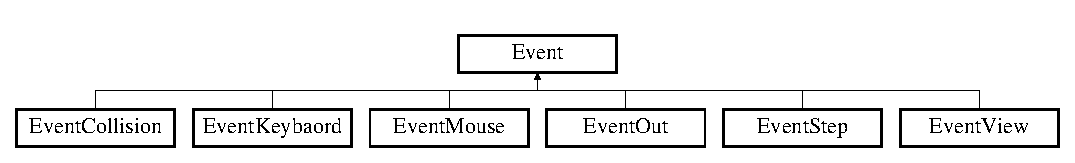
\includegraphics[height=1.744548cm]{class_event}
\end{center}
\end{figure}
\subsection*{Public Member Functions}
\begin{DoxyCompactItemize}
\item 
\hyperlink{class_event_a5a40dd4708297f7031e29b39e039ae10}{Event} ()
\item 
virtual \hyperlink{class_event_a7704ec01ce91e673885792054214b3d2}{$\sim$\+Event} ()
\item 
void \hyperlink{class_event_a6eb2f305445ab6d86e64acaacf145ab2}{set\+Type} (string new\+\_\+type)
\item 
string \hyperlink{class_event_a33f3769ef82c06a638a2640a4fe0fef3}{get\+Type} () const 
\end{DoxyCompactItemize}


\subsection{Detailed Description}
The base class for sending events to objects 

\subsection{Constructor \& Destructor Documentation}
\hypertarget{class_event_a5a40dd4708297f7031e29b39e039ae10}{\index{Event@{Event}!Event@{Event}}
\index{Event@{Event}!Event@{Event}}
\subsubsection[{Event}]{\setlength{\rightskip}{0pt plus 5cm}Event\+::\+Event (
\begin{DoxyParamCaption}
{}
\end{DoxyParamCaption}
)}}\label{class_event_a5a40dd4708297f7031e29b39e039ae10}
Create a new event \hypertarget{class_event_a7704ec01ce91e673885792054214b3d2}{\index{Event@{Event}!````~Event@{$\sim$\+Event}}
\index{````~Event@{$\sim$\+Event}!Event@{Event}}
\subsubsection[{$\sim$\+Event}]{\setlength{\rightskip}{0pt plus 5cm}Event\+::$\sim$\+Event (
\begin{DoxyParamCaption}
{}
\end{DoxyParamCaption}
)\hspace{0.3cm}{\ttfamily [virtual]}}}\label{class_event_a7704ec01ce91e673885792054214b3d2}
Called when the event is deleted 

\subsection{Member Function Documentation}
\hypertarget{class_event_a33f3769ef82c06a638a2640a4fe0fef3}{\index{Event@{Event}!get\+Type@{get\+Type}}
\index{get\+Type@{get\+Type}!Event@{Event}}
\subsubsection[{get\+Type}]{\setlength{\rightskip}{0pt plus 5cm}string Event\+::get\+Type (
\begin{DoxyParamCaption}
{}
\end{DoxyParamCaption}
) const}}\label{class_event_a33f3769ef82c06a638a2640a4fe0fef3}
Get the type that this event is \begin{DoxyReturn}{Returns}
The type name of this event 
\end{DoxyReturn}
\hypertarget{class_event_a6eb2f305445ab6d86e64acaacf145ab2}{\index{Event@{Event}!set\+Type@{set\+Type}}
\index{set\+Type@{set\+Type}!Event@{Event}}
\subsubsection[{set\+Type}]{\setlength{\rightskip}{0pt plus 5cm}void Event\+::set\+Type (
\begin{DoxyParamCaption}
\item[{string}]{new\+\_\+type}
\end{DoxyParamCaption}
)}}\label{class_event_a6eb2f305445ab6d86e64acaacf145ab2}
Change the type of the event 
\begin{DoxyParams}{Parameters}
{\em new\+\_\+type} & The new type that this event should be \\
\hline
\end{DoxyParams}


The documentation for this class was generated from the following files\+:\begin{DoxyCompactItemize}
\item 
F\+:/\+Users/\+Benny/git/\+I\+M\+G\+D3000/\+I\+M\+G\+D3000\+Proj3/include/Event.\+h\item 
F\+:/\+Users/\+Benny/git/\+I\+M\+G\+D3000/\+I\+M\+G\+D3000\+Proj3/lib/src/\+Core/Event.\+cpp\end{DoxyCompactItemize}

\hypertarget{class_event_collision}{\section{Event\+Collision Class Reference}
\label{class_event_collision}\index{Event\+Collision@{Event\+Collision}}
}


{\ttfamily \#include $<$Event\+Collision.\+h$>$}

Inheritance diagram for Event\+Collision\+:\begin{figure}[H]
\begin{center}
\leavevmode
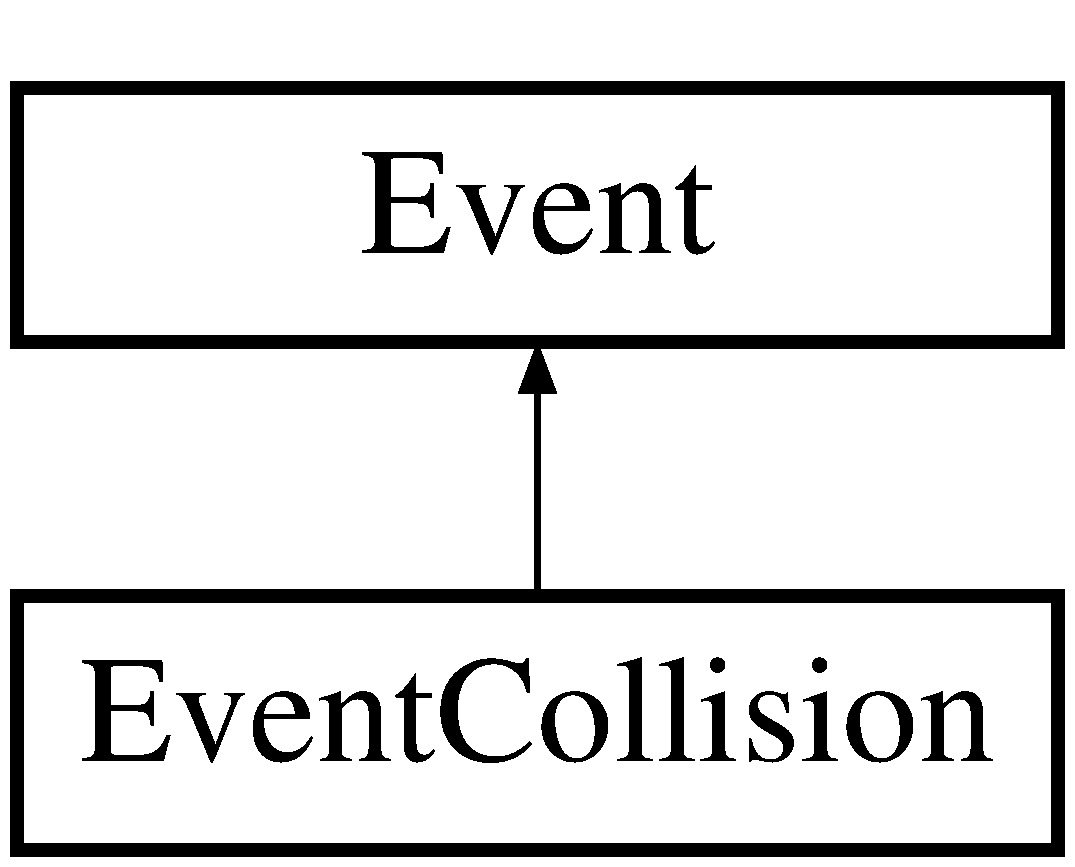
\includegraphics[height=2.000000cm]{class_event_collision}
\end{center}
\end{figure}
\subsection*{Public Member Functions}
\begin{DoxyCompactItemize}
\item 
\hyperlink{class_event_collision_a7351501bd297d82811deed639c3c6d3d}{Event\+Collision} (\hyperlink{class_i_vector}{I\+Vector} position, \hyperlink{class_object}{Object} $\ast$obj1, \hyperlink{class_object}{Object} $\ast$obj2)
\item 
\hyperlink{class_i_vector}{I\+Vector} \hyperlink{class_event_collision_a9ed1a0fd9cc1006ef8a25574c5bb5a69}{get\+Position} ()
\item 
\hyperlink{class_object}{Object} $\ast$ \hyperlink{class_event_collision_a74ac21fbda77c2ffb080a0228178b5ae}{get\+Obj1} () const 
\item 
\hyperlink{class_object}{Object} $\ast$ \hyperlink{class_event_collision_a57b819fcb05e03b7b9ca41631881b909}{get\+Obj2} () const 
\end{DoxyCompactItemize}


\subsection{Detailed Description}
An event that is fired whenever a collision happens This event is not global, it will only be fired on objects involved in the collision 

\subsection{Constructor \& Destructor Documentation}
\hypertarget{class_event_collision_a7351501bd297d82811deed639c3c6d3d}{\index{Event\+Collision@{Event\+Collision}!Event\+Collision@{Event\+Collision}}
\index{Event\+Collision@{Event\+Collision}!Event\+Collision@{Event\+Collision}}
\subsubsection[{Event\+Collision}]{\setlength{\rightskip}{0pt plus 5cm}Event\+Collision\+::\+Event\+Collision (
\begin{DoxyParamCaption}
\item[{{\bf I\+Vector}}]{position, }
\item[{{\bf Object} $\ast$}]{obj1, }
\item[{{\bf Object} $\ast$}]{obj2}
\end{DoxyParamCaption}
)}}\label{class_event_collision_a7351501bd297d82811deed639c3c6d3d}
Creates a new collision event 
\begin{DoxyParams}{Parameters}
{\em position} & The position that the collision was at \\
\hline
{\em obj1} & The first object in the collision \\
\hline
{\em obj2} & The second object in the collision \\
\hline
\end{DoxyParams}


\subsection{Member Function Documentation}
\hypertarget{class_event_collision_a74ac21fbda77c2ffb080a0228178b5ae}{\index{Event\+Collision@{Event\+Collision}!get\+Obj1@{get\+Obj1}}
\index{get\+Obj1@{get\+Obj1}!Event\+Collision@{Event\+Collision}}
\subsubsection[{get\+Obj1}]{\setlength{\rightskip}{0pt plus 5cm}{\bf Object} $\ast$ Event\+Collision\+::get\+Obj1 (
\begin{DoxyParamCaption}
{}
\end{DoxyParamCaption}
) const}}\label{class_event_collision_a74ac21fbda77c2ffb080a0228178b5ae}
Gets the first object involved in the collision \begin{DoxyReturn}{Returns}
The first object involved in the collision 
\end{DoxyReturn}
\hypertarget{class_event_collision_a57b819fcb05e03b7b9ca41631881b909}{\index{Event\+Collision@{Event\+Collision}!get\+Obj2@{get\+Obj2}}
\index{get\+Obj2@{get\+Obj2}!Event\+Collision@{Event\+Collision}}
\subsubsection[{get\+Obj2}]{\setlength{\rightskip}{0pt plus 5cm}{\bf Object} $\ast$ Event\+Collision\+::get\+Obj2 (
\begin{DoxyParamCaption}
{}
\end{DoxyParamCaption}
) const}}\label{class_event_collision_a57b819fcb05e03b7b9ca41631881b909}
Gets the second object involved in the collision \begin{DoxyReturn}{Returns}
The second object involved in the collision 
\end{DoxyReturn}
\hypertarget{class_event_collision_a9ed1a0fd9cc1006ef8a25574c5bb5a69}{\index{Event\+Collision@{Event\+Collision}!get\+Position@{get\+Position}}
\index{get\+Position@{get\+Position}!Event\+Collision@{Event\+Collision}}
\subsubsection[{get\+Position}]{\setlength{\rightskip}{0pt plus 5cm}{\bf I\+Vector} Event\+Collision\+::get\+Position (
\begin{DoxyParamCaption}
{}
\end{DoxyParamCaption}
)}}\label{class_event_collision_a9ed1a0fd9cc1006ef8a25574c5bb5a69}
The position the collision was at \begin{DoxyReturn}{Returns}
An \hyperlink{class_i_vector}{I\+Vector} that represents the world location that the collision was at 
\end{DoxyReturn}


The documentation for this class was generated from the following files\+:\begin{DoxyCompactItemize}
\item 
F\+:/\+Users/\+Benny/git/\+I\+M\+G\+D3000/\+I\+M\+G\+D3000\+Proj3/include/Event\+Collision.\+h\item 
F\+:/\+Users/\+Benny/git/\+I\+M\+G\+D3000/\+I\+M\+G\+D3000\+Proj3/lib/src/\+Physics/Event\+Collision.\+cpp\end{DoxyCompactItemize}

\hypertarget{class_event_keybaord}{\section{Event\+Keybaord Class Reference}
\label{class_event_keybaord}\index{Event\+Keybaord@{Event\+Keybaord}}
}


{\ttfamily \#include $<$Event\+Keybaord.\+h$>$}

Inheritance diagram for Event\+Keybaord\+:\begin{figure}[H]
\begin{center}
\leavevmode
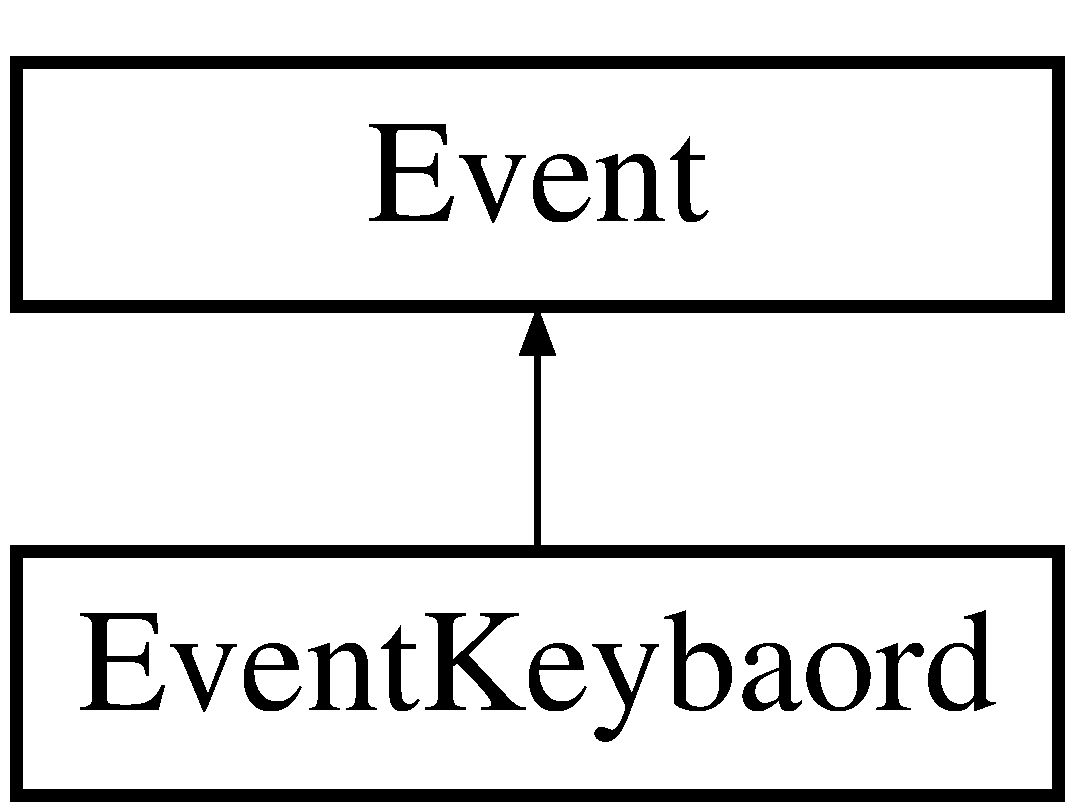
\includegraphics[height=2.000000cm]{class_event_keybaord}
\end{center}
\end{figure}
\subsection*{Public Member Functions}
\begin{DoxyCompactItemize}
\item 
\hyperlink{class_event_keybaord_ab4859a0213a93565767b4cc8ca0743d2}{Event\+Keybaord} (int key)
\item 
int \hyperlink{class_event_keybaord_acef0f3223a83760c45b8ee8d0f28d237}{get\+Key} () const 
\end{DoxyCompactItemize}


\subsection{Detailed Description}
\hyperlink{class_event}{Event} called whenever there is a keyboard event 

\subsection{Constructor \& Destructor Documentation}
\hypertarget{class_event_keybaord_ab4859a0213a93565767b4cc8ca0743d2}{\index{Event\+Keybaord@{Event\+Keybaord}!Event\+Keybaord@{Event\+Keybaord}}
\index{Event\+Keybaord@{Event\+Keybaord}!Event\+Keybaord@{Event\+Keybaord}}
\subsubsection[{Event\+Keybaord}]{\setlength{\rightskip}{0pt plus 5cm}Event\+Keybaord\+::\+Event\+Keybaord (
\begin{DoxyParamCaption}
\item[{int}]{key}
\end{DoxyParamCaption}
)}}\label{class_event_keybaord_ab4859a0213a93565767b4cc8ca0743d2}
Creates a new keyboard event 
\begin{DoxyParams}{Parameters}
{\em key} & The key value that was pressed \\
\hline
\end{DoxyParams}


\subsection{Member Function Documentation}
\hypertarget{class_event_keybaord_acef0f3223a83760c45b8ee8d0f28d237}{\index{Event\+Keybaord@{Event\+Keybaord}!get\+Key@{get\+Key}}
\index{get\+Key@{get\+Key}!Event\+Keybaord@{Event\+Keybaord}}
\subsubsection[{get\+Key}]{\setlength{\rightskip}{0pt plus 5cm}int Event\+Keybaord\+::get\+Key (
\begin{DoxyParamCaption}
{}
\end{DoxyParamCaption}
) const}}\label{class_event_keybaord_acef0f3223a83760c45b8ee8d0f28d237}
Gets the key value of this event \begin{DoxyReturn}{Returns}
An integer representing the key value 
\end{DoxyReturn}


The documentation for this class was generated from the following files\+:\begin{DoxyCompactItemize}
\item 
F\+:/\+Users/\+Benny/git/\+I\+M\+G\+D3000/\+I\+M\+G\+D3000\+Proj3/include/Event\+Keybaord.\+h\item 
F\+:/\+Users/\+Benny/git/\+I\+M\+G\+D3000/\+I\+M\+G\+D3000\+Proj3/lib/src/\+Input/Event\+Keybaord.\+cpp\end{DoxyCompactItemize}

\hypertarget{class_event_mouse}{\section{Event\+Mouse Class Reference}
\label{class_event_mouse}\index{Event\+Mouse@{Event\+Mouse}}
}


{\ttfamily \#include $<$Event\+Mouse.\+h$>$}

Inheritance diagram for Event\+Mouse\+:\begin{figure}[H]
\begin{center}
\leavevmode
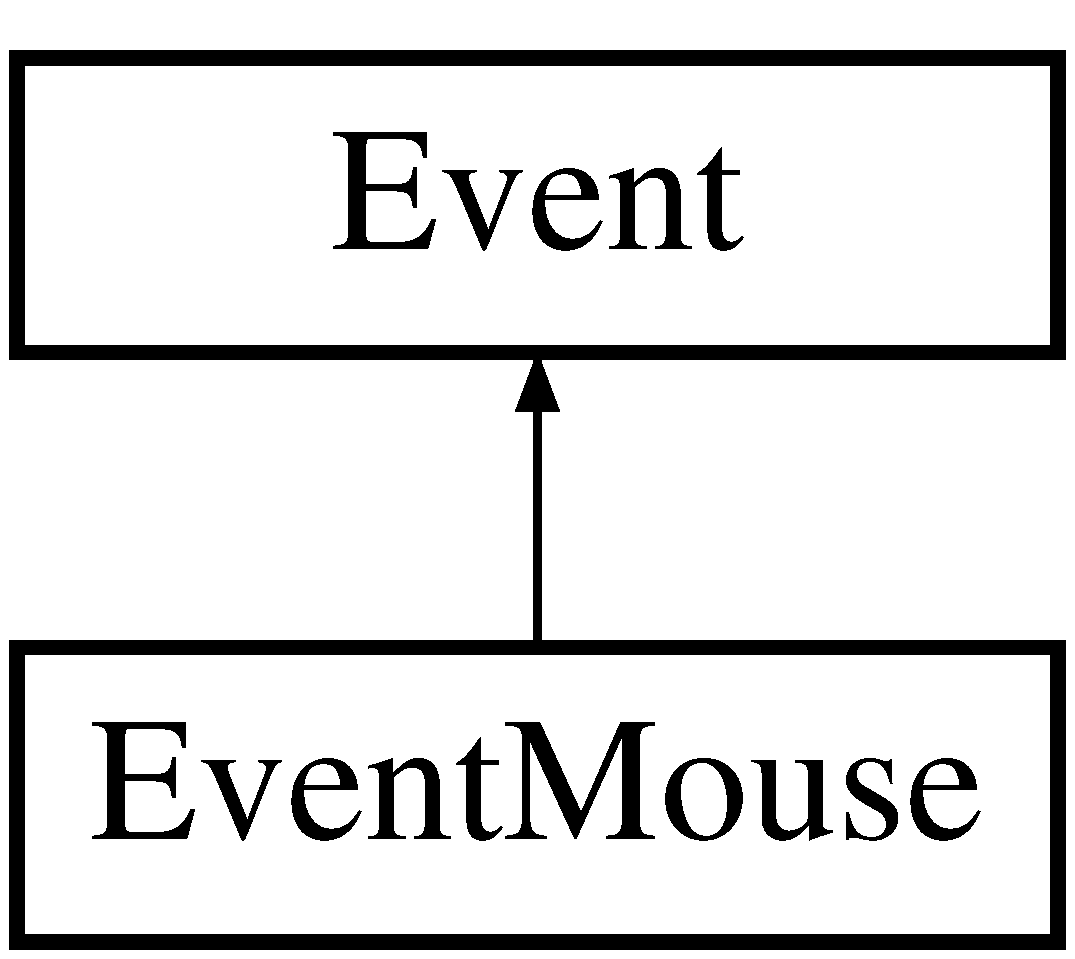
\includegraphics[height=2.000000cm]{class_event_mouse}
\end{center}
\end{figure}
\subsection*{Public Member Functions}
\begin{DoxyCompactItemize}
\item 
\hyperlink{class_event_mouse_a57af369efaecf3f4c4ded4d3543720cb}{Event\+Mouse} (int x, int y, Mouse\+Action\+List action)
\item 
int \hyperlink{class_event_mouse_a9cc157a57d229748d2261ef05df16188}{get\+X} () const 
\item 
int \hyperlink{class_event_mouse_a5a23acf16c866cf5c8adc9ffcf2445be}{get\+Y} () const 
\item 
Mouse\+Action\+List \hyperlink{class_event_mouse_a8172862dd288ce9555b486f542ed2fe3}{get\+Mouse\+Action} () const 
\end{DoxyCompactItemize}


\subsection{Detailed Description}
\hyperlink{class_event}{Event} sent whenever there is a mouse event 

\subsection{Constructor \& Destructor Documentation}
\hypertarget{class_event_mouse_a57af369efaecf3f4c4ded4d3543720cb}{\index{Event\+Mouse@{Event\+Mouse}!Event\+Mouse@{Event\+Mouse}}
\index{Event\+Mouse@{Event\+Mouse}!Event\+Mouse@{Event\+Mouse}}
\subsubsection[{Event\+Mouse}]{\setlength{\rightskip}{0pt plus 5cm}Event\+Mouse\+::\+Event\+Mouse (
\begin{DoxyParamCaption}
\item[{int}]{x, }
\item[{int}]{y, }
\item[{Mouse\+Action\+List}]{action}
\end{DoxyParamCaption}
)}}\label{class_event_mouse_a57af369efaecf3f4c4ded4d3543720cb}
Creates a new mouse event 
\begin{DoxyParams}{Parameters}
{\em x} & The x location of the mouse \\
\hline
{\em y} & The y location of the mouse \\
\hline
{\em action} & The button or action that the mouse did to trigger this event \\
\hline
\end{DoxyParams}


\subsection{Member Function Documentation}
\hypertarget{class_event_mouse_a8172862dd288ce9555b486f542ed2fe3}{\index{Event\+Mouse@{Event\+Mouse}!get\+Mouse\+Action@{get\+Mouse\+Action}}
\index{get\+Mouse\+Action@{get\+Mouse\+Action}!Event\+Mouse@{Event\+Mouse}}
\subsubsection[{get\+Mouse\+Action}]{\setlength{\rightskip}{0pt plus 5cm}Mouse\+Action\+List Event\+Mouse\+::get\+Mouse\+Action (
\begin{DoxyParamCaption}
{}
\end{DoxyParamCaption}
) const}}\label{class_event_mouse_a8172862dd288ce9555b486f542ed2fe3}
Get the mouse action that was used to trigger this event \begin{DoxyReturn}{Returns}
The mouse action 
\end{DoxyReturn}
\hypertarget{class_event_mouse_a9cc157a57d229748d2261ef05df16188}{\index{Event\+Mouse@{Event\+Mouse}!get\+X@{get\+X}}
\index{get\+X@{get\+X}!Event\+Mouse@{Event\+Mouse}}
\subsubsection[{get\+X}]{\setlength{\rightskip}{0pt plus 5cm}int Event\+Mouse\+::get\+X (
\begin{DoxyParamCaption}
{}
\end{DoxyParamCaption}
) const}}\label{class_event_mouse_a9cc157a57d229748d2261ef05df16188}
Get the x location of the mouse when this event was fired \begin{DoxyReturn}{Returns}
An integer representing the mouse x location 
\end{DoxyReturn}
\hypertarget{class_event_mouse_a5a23acf16c866cf5c8adc9ffcf2445be}{\index{Event\+Mouse@{Event\+Mouse}!get\+Y@{get\+Y}}
\index{get\+Y@{get\+Y}!Event\+Mouse@{Event\+Mouse}}
\subsubsection[{get\+Y}]{\setlength{\rightskip}{0pt plus 5cm}int Event\+Mouse\+::get\+Y (
\begin{DoxyParamCaption}
{}
\end{DoxyParamCaption}
) const}}\label{class_event_mouse_a5a23acf16c866cf5c8adc9ffcf2445be}
Get the y location of the mouse when this event was fired \begin{DoxyReturn}{Returns}
An integer representing the mouse y location 
\end{DoxyReturn}


The documentation for this class was generated from the following files\+:\begin{DoxyCompactItemize}
\item 
F\+:/\+Users/\+Benny/git/\+I\+M\+G\+D3000/\+I\+M\+G\+D3000\+Proj3/include/Event\+Mouse.\+h\item 
F\+:/\+Users/\+Benny/git/\+I\+M\+G\+D3000/\+I\+M\+G\+D3000\+Proj3/lib/src/\+Input/Event\+Mouse.\+cpp\end{DoxyCompactItemize}

\hypertarget{class_event_out}{\section{Event\+Out Class Reference}
\label{class_event_out}\index{Event\+Out@{Event\+Out}}
}
Inheritance diagram for Event\+Out\+:\begin{figure}[H]
\begin{center}
\leavevmode
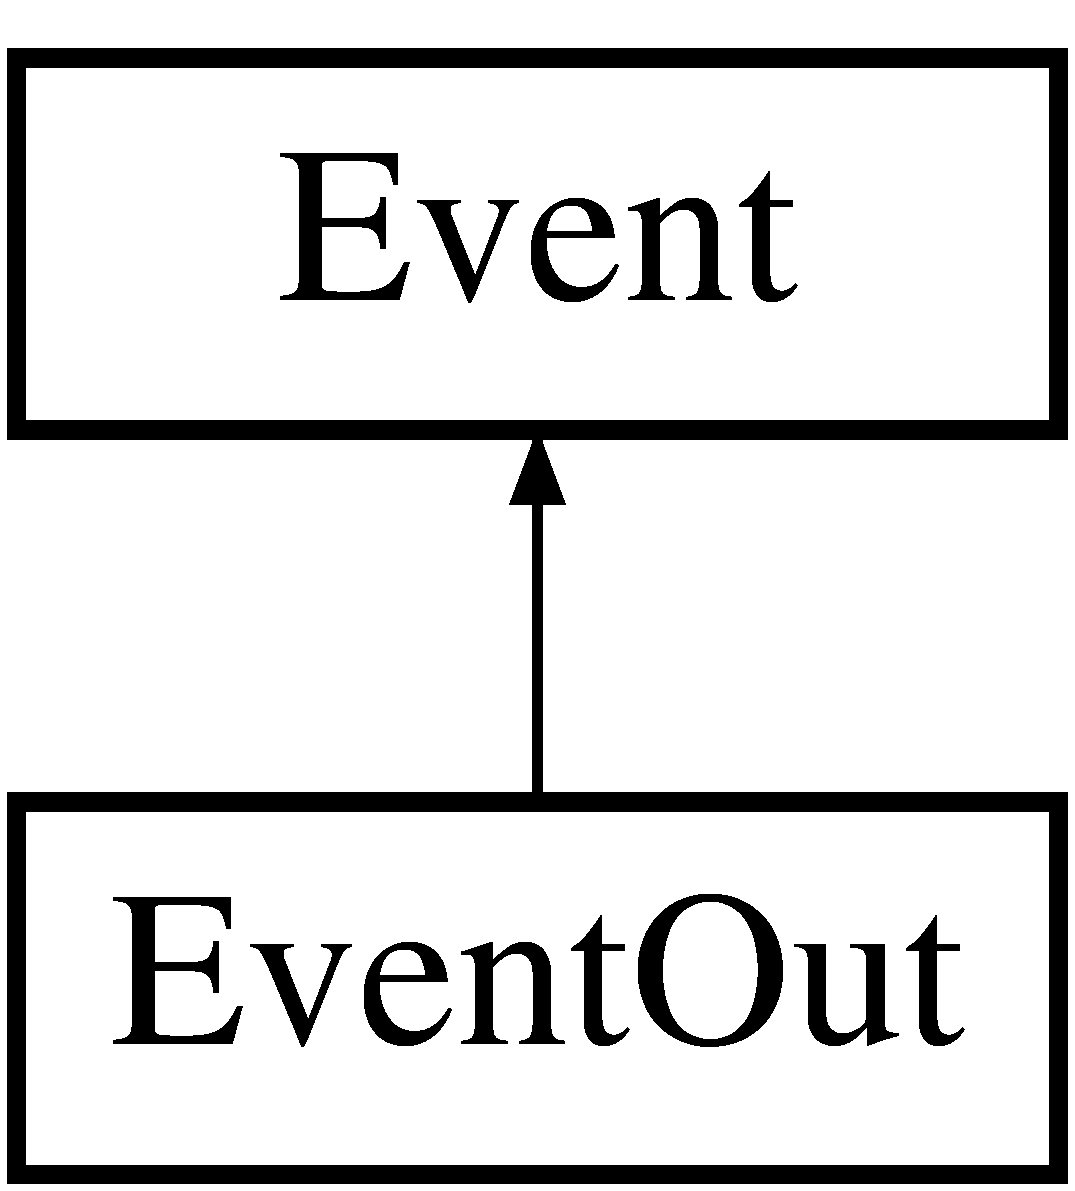
\includegraphics[height=2.000000cm]{class_event_out}
\end{center}
\end{figure}
\subsection*{Additional Inherited Members}


The documentation for this class was generated from the following files\+:\begin{DoxyCompactItemize}
\item 
F\+:/\+Users/\+Benny/git/\+I\+M\+G\+D3000/\+I\+M\+G\+D3000\+Proj3/include/Event\+Out.\+h\item 
F\+:/\+Users/\+Benny/git/\+I\+M\+G\+D3000/\+I\+M\+G\+D3000\+Proj3/lib/src/\+Game/Event\+Out.\+cpp\end{DoxyCompactItemize}

\hypertarget{class_event_step}{\section{Event\+Step Class Reference}
\label{class_event_step}\index{Event\+Step@{Event\+Step}}
}


{\ttfamily \#include $<$Event\+Step.\+h$>$}

Inheritance diagram for Event\+Step\+:\begin{figure}[H]
\begin{center}
\leavevmode
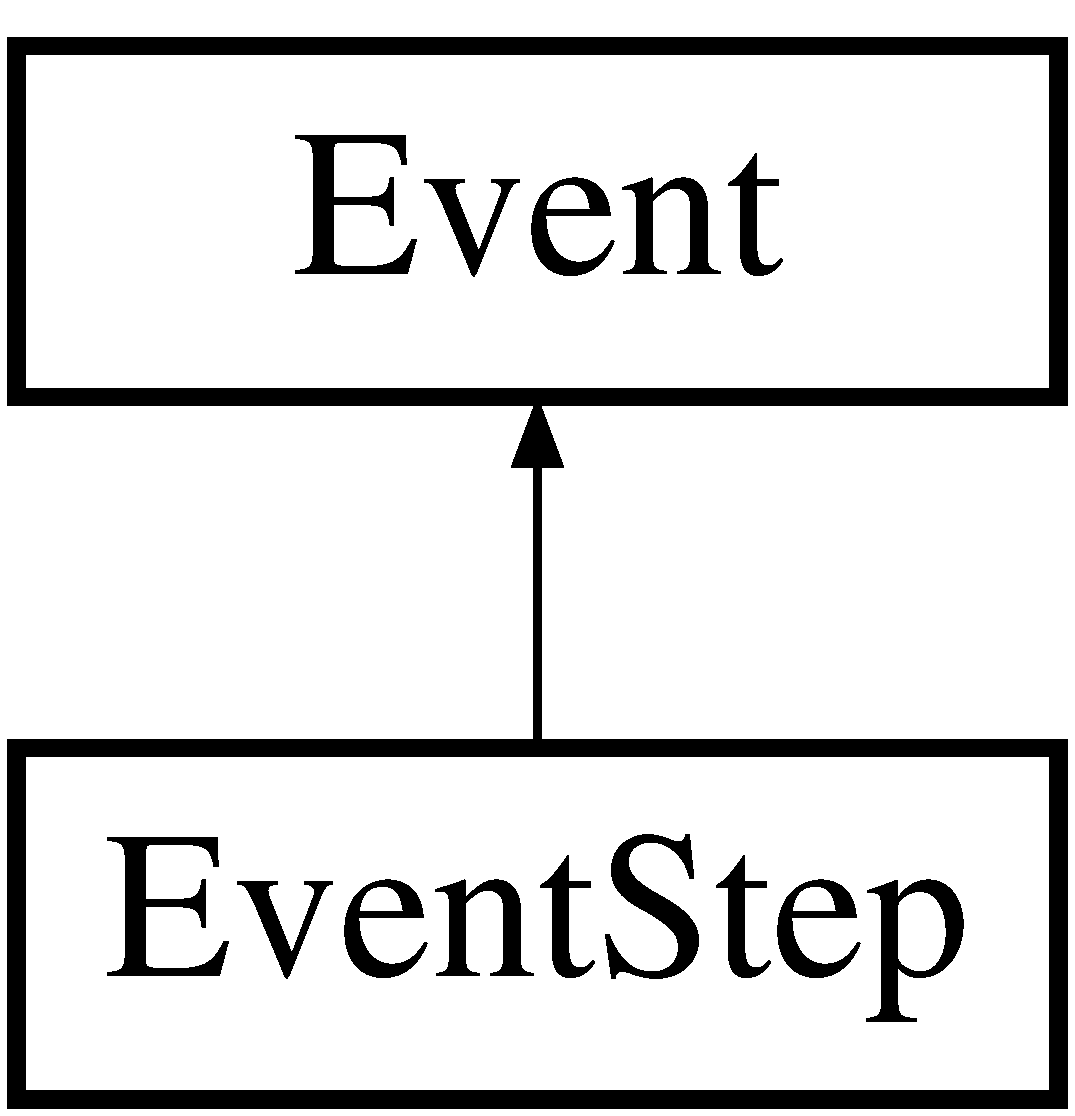
\includegraphics[height=2.000000cm]{class_event_step}
\end{center}
\end{figure}
\subsection*{Public Member Functions}
\begin{DoxyCompactItemize}
\item 
\hyperlink{class_event_step_a00df7973f32444b8e0d677ce2a3e34b1}{Event\+Step} (unsigned int step\+Count)
\item 
virtual \hyperlink{class_event_step_a1fd5402baa54bf82bac6bc8b6f3a84d1}{$\sim$\+Event\+Step} ()
\item 
unsigned int \hyperlink{class_event_step_a39878b3b58788d25012b417f5863c254}{get\+Step\+Count} () const 
\end{DoxyCompactItemize}


\subsection{Detailed Description}
\hyperlink{class_event}{Event} called every step 

\subsection{Constructor \& Destructor Documentation}
\hypertarget{class_event_step_a00df7973f32444b8e0d677ce2a3e34b1}{\index{Event\+Step@{Event\+Step}!Event\+Step@{Event\+Step}}
\index{Event\+Step@{Event\+Step}!Event\+Step@{Event\+Step}}
\subsubsection[{Event\+Step}]{\setlength{\rightskip}{0pt plus 5cm}Event\+Step\+::\+Event\+Step (
\begin{DoxyParamCaption}
\item[{unsigned int}]{step\+Count}
\end{DoxyParamCaption}
)}}\label{class_event_step_a00df7973f32444b8e0d677ce2a3e34b1}
Creates a new step event 
\begin{DoxyParams}{Parameters}
{\em step\+Count} & The number step this is in the engine sense startup \\
\hline
\end{DoxyParams}
\hypertarget{class_event_step_a1fd5402baa54bf82bac6bc8b6f3a84d1}{\index{Event\+Step@{Event\+Step}!````~Event\+Step@{$\sim$\+Event\+Step}}
\index{````~Event\+Step@{$\sim$\+Event\+Step}!Event\+Step@{Event\+Step}}
\subsubsection[{$\sim$\+Event\+Step}]{\setlength{\rightskip}{0pt plus 5cm}Event\+Step\+::$\sim$\+Event\+Step (
\begin{DoxyParamCaption}
{}
\end{DoxyParamCaption}
)\hspace{0.3cm}{\ttfamily [virtual]}}}\label{class_event_step_a1fd5402baa54bf82bac6bc8b6f3a84d1}
Called when the step event is killed 

\subsection{Member Function Documentation}
\hypertarget{class_event_step_a39878b3b58788d25012b417f5863c254}{\index{Event\+Step@{Event\+Step}!get\+Step\+Count@{get\+Step\+Count}}
\index{get\+Step\+Count@{get\+Step\+Count}!Event\+Step@{Event\+Step}}
\subsubsection[{get\+Step\+Count}]{\setlength{\rightskip}{0pt plus 5cm}unsigned int Event\+Step\+::get\+Step\+Count (
\begin{DoxyParamCaption}
{}
\end{DoxyParamCaption}
) const}}\label{class_event_step_a39878b3b58788d25012b417f5863c254}
Get the step count from this event \begin{DoxyReturn}{Returns}
An unsigned int representing the step count 
\end{DoxyReturn}


The documentation for this class was generated from the following files\+:\begin{DoxyCompactItemize}
\item 
F\+:/\+Users/\+Benny/git/\+I\+M\+G\+D3000/\+I\+M\+G\+D3000\+Proj3/include/Event\+Step.\+h\item 
F\+:/\+Users/\+Benny/git/\+I\+M\+G\+D3000/\+I\+M\+G\+D3000\+Proj3/lib/src/\+Core/Event\+Step.\+cpp\end{DoxyCompactItemize}

\hypertarget{class_event_view}{\section{Event\+View Class Reference}
\label{class_event_view}\index{Event\+View@{Event\+View}}
}


{\ttfamily \#include $<$Event\+View.\+h$>$}

Inheritance diagram for Event\+View\+:\begin{figure}[H]
\begin{center}
\leavevmode
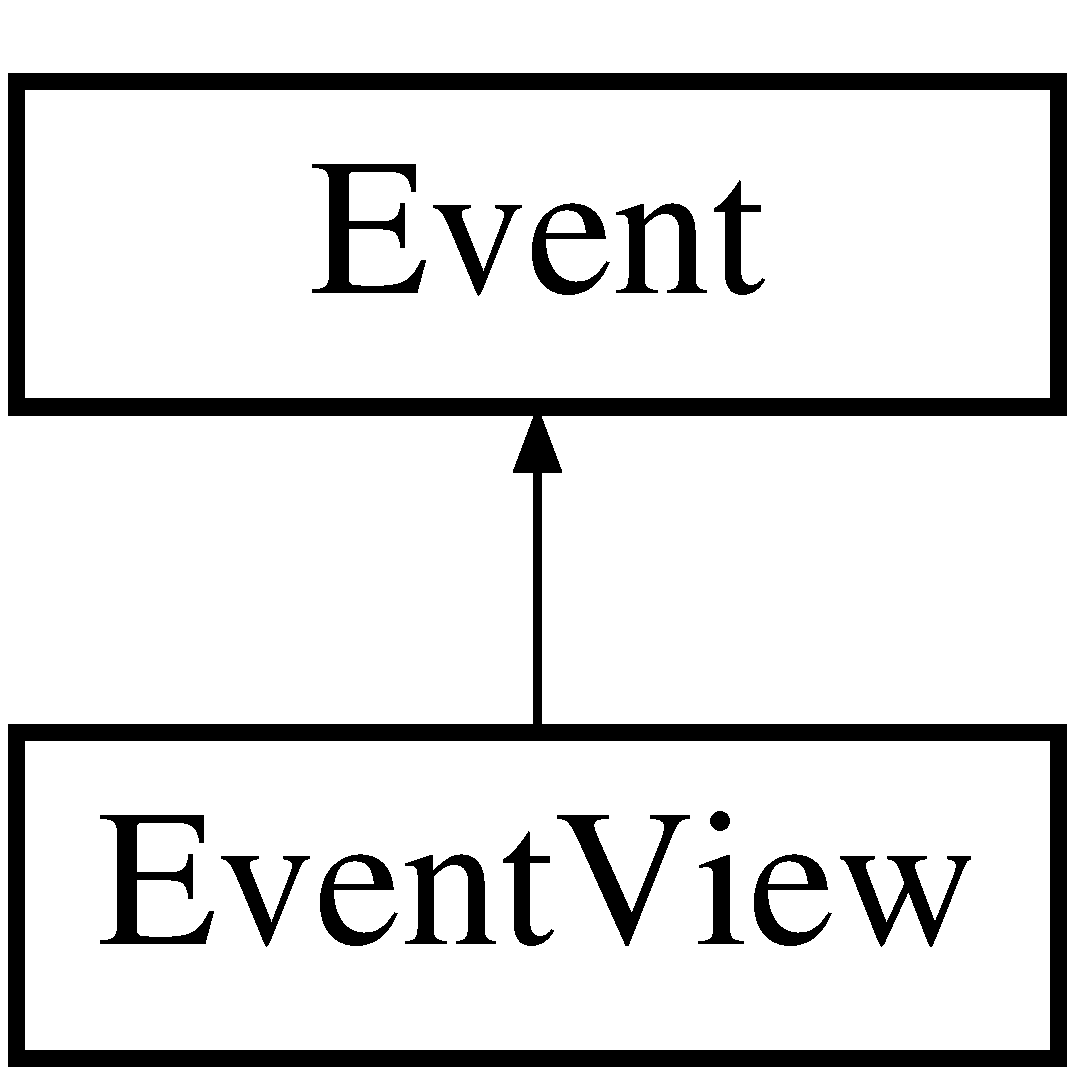
\includegraphics[height=2.000000cm]{class_event_view}
\end{center}
\end{figure}
\subsection*{Public Member Functions}
\begin{DoxyCompactItemize}
\item 
\hyperlink{class_event_view_a6c8e67589e2b938db9139dcb6eaeabd6}{Event\+View} (string tag, int value, bool delta=true)
\item 
string \hyperlink{class_event_view_a5f737dfd3a000cb45192aa56113afd59}{get\+Tag} () const 
\item 
int \hyperlink{class_event_view_a5e7381f571d0cc269df58b1de2db5620}{get\+Value} () const 
\item 
bool \hyperlink{class_event_view_af72a798337d18edbaa8c366b1e353b85}{get\+Delta} () const 
\end{DoxyCompactItemize}


\subsection{Detailed Description}
An event used to modify U\+I elements 

\subsection{Constructor \& Destructor Documentation}
\hypertarget{class_event_view_a6c8e67589e2b938db9139dcb6eaeabd6}{\index{Event\+View@{Event\+View}!Event\+View@{Event\+View}}
\index{Event\+View@{Event\+View}!Event\+View@{Event\+View}}
\subsubsection[{Event\+View}]{\setlength{\rightskip}{0pt plus 5cm}Event\+View\+::\+Event\+View (
\begin{DoxyParamCaption}
\item[{string}]{tag, }
\item[{int}]{value, }
\item[{bool}]{delta = {\ttfamily true}}
\end{DoxyParamCaption}
)}}\label{class_event_view_a6c8e67589e2b938db9139dcb6eaeabd6}
Creates a new view event 
\begin{DoxyParams}{Parameters}
{\em tag} & The tag on the U\+I element that this event should apply to \\
\hline
{\em value} & The value to modify the tag with \\
\hline
{\em delta} & If true then we will add value to the current value of the U\+I element, if false then we will just set \\
\hline
\end{DoxyParams}


\subsection{Member Function Documentation}
\hypertarget{class_event_view_af72a798337d18edbaa8c366b1e353b85}{\index{Event\+View@{Event\+View}!get\+Delta@{get\+Delta}}
\index{get\+Delta@{get\+Delta}!Event\+View@{Event\+View}}
\subsubsection[{get\+Delta}]{\setlength{\rightskip}{0pt plus 5cm}bool Event\+View\+::get\+Delta (
\begin{DoxyParamCaption}
{}
\end{DoxyParamCaption}
) const}}\label{class_event_view_af72a798337d18edbaa8c366b1e353b85}
Check to see if this event should only increment the value of the U\+I element \begin{DoxyReturn}{Returns}
If true then we will only increment the value, otherwise we will set it 
\end{DoxyReturn}
\hypertarget{class_event_view_a5f737dfd3a000cb45192aa56113afd59}{\index{Event\+View@{Event\+View}!get\+Tag@{get\+Tag}}
\index{get\+Tag@{get\+Tag}!Event\+View@{Event\+View}}
\subsubsection[{get\+Tag}]{\setlength{\rightskip}{0pt plus 5cm}string Event\+View\+::get\+Tag (
\begin{DoxyParamCaption}
{}
\end{DoxyParamCaption}
) const}}\label{class_event_view_a5f737dfd3a000cb45192aa56113afd59}
Get the tag on this event \begin{DoxyReturn}{Returns}
The tag of the U\+I object that this event applies to 
\end{DoxyReturn}
\hypertarget{class_event_view_a5e7381f571d0cc269df58b1de2db5620}{\index{Event\+View@{Event\+View}!get\+Value@{get\+Value}}
\index{get\+Value@{get\+Value}!Event\+View@{Event\+View}}
\subsubsection[{get\+Value}]{\setlength{\rightskip}{0pt plus 5cm}int Event\+View\+::get\+Value (
\begin{DoxyParamCaption}
{}
\end{DoxyParamCaption}
) const}}\label{class_event_view_a5e7381f571d0cc269df58b1de2db5620}
Get the value stored in this event \begin{DoxyReturn}{Returns}
The value to modify the U\+I element with 
\end{DoxyReturn}


The documentation for this class was generated from the following files\+:\begin{DoxyCompactItemize}
\item 
F\+:/\+Users/\+Benny/git/\+I\+M\+G\+D3000/\+I\+M\+G\+D3000\+Proj3/include/Event\+View.\+h\item 
F\+:/\+Users/\+Benny/git/\+I\+M\+G\+D3000/\+I\+M\+G\+D3000\+Proj3/lib/src/\+Object/Event\+View.\+cpp\end{DoxyCompactItemize}

\hypertarget{class_frame}{\section{Frame Class Reference}
\label{class_frame}\index{Frame@{Frame}}
}


{\ttfamily \#include $<$Frame.\+h$>$}

\subsection*{Public Member Functions}
\begin{DoxyCompactItemize}
\item 
\hyperlink{class_frame_ad2e5946cf41d4817e750500acf05d02b}{Frame} ()
\item 
\hyperlink{class_frame_a04960e256aeb88ea7594044b004d1d4f}{Frame} (int width, int height, string str)
\item 
int \hyperlink{class_frame_a6fdc35835bac73cebb16e5f9410f69a7}{get\+Width} () const 
\item 
int \hyperlink{class_frame_a01ee67899972b90ed68a86e9e741dd63}{get\+Height} () const 
\item 
void \hyperlink{class_frame_aa5399c4706ebfe13a7c9f2672855fb9b}{set\+Width} (int width)
\item 
void \hyperlink{class_frame_a88223ca58969c74eb0bf1710287229f6}{set\+Height} (int height)
\item 
string \hyperlink{class_frame_ab30188fbbd660c4f10dea8e038401b6a}{get\+String} () const 
\item 
void \hyperlink{class_frame_a54dd23fa6e469b2f6bf0a540a2e4e348}{set\+String} (string new\+Str)
\end{DoxyCompactItemize}


\subsection{Detailed Description}
A single frame of a sprite 

\subsection{Constructor \& Destructor Documentation}
\hypertarget{class_frame_ad2e5946cf41d4817e750500acf05d02b}{\index{Frame@{Frame}!Frame@{Frame}}
\index{Frame@{Frame}!Frame@{Frame}}
\subsubsection[{Frame}]{\setlength{\rightskip}{0pt plus 5cm}Frame\+::\+Frame (
\begin{DoxyParamCaption}
{}
\end{DoxyParamCaption}
)}}\label{class_frame_ad2e5946cf41d4817e750500acf05d02b}
Creates an empty frame \hypertarget{class_frame_a04960e256aeb88ea7594044b004d1d4f}{\index{Frame@{Frame}!Frame@{Frame}}
\index{Frame@{Frame}!Frame@{Frame}}
\subsubsection[{Frame}]{\setlength{\rightskip}{0pt plus 5cm}Frame\+::\+Frame (
\begin{DoxyParamCaption}
\item[{int}]{width, }
\item[{int}]{height, }
\item[{string}]{str}
\end{DoxyParamCaption}
)}}\label{class_frame_a04960e256aeb88ea7594044b004d1d4f}
Creates a new frame 
\begin{DoxyParams}{Parameters}
{\em width} & The width of the frame \\
\hline
{\em height} & The height of the frame \\
\hline
{\em str} & The characters that compose the frame \\
\hline
\end{DoxyParams}


\subsection{Member Function Documentation}
\hypertarget{class_frame_a01ee67899972b90ed68a86e9e741dd63}{\index{Frame@{Frame}!get\+Height@{get\+Height}}
\index{get\+Height@{get\+Height}!Frame@{Frame}}
\subsubsection[{get\+Height}]{\setlength{\rightskip}{0pt plus 5cm}int Frame\+::get\+Height (
\begin{DoxyParamCaption}
{}
\end{DoxyParamCaption}
) const}}\label{class_frame_a01ee67899972b90ed68a86e9e741dd63}
Gets the height of the frame \begin{DoxyReturn}{Returns}
The height of the frame 
\end{DoxyReturn}
\hypertarget{class_frame_ab30188fbbd660c4f10dea8e038401b6a}{\index{Frame@{Frame}!get\+String@{get\+String}}
\index{get\+String@{get\+String}!Frame@{Frame}}
\subsubsection[{get\+String}]{\setlength{\rightskip}{0pt plus 5cm}string Frame\+::get\+String (
\begin{DoxyParamCaption}
{}
\end{DoxyParamCaption}
) const}}\label{class_frame_ab30188fbbd660c4f10dea8e038401b6a}
Get the string that this frame uses \begin{DoxyReturn}{Returns}
The string for this frame 
\end{DoxyReturn}
\hypertarget{class_frame_a6fdc35835bac73cebb16e5f9410f69a7}{\index{Frame@{Frame}!get\+Width@{get\+Width}}
\index{get\+Width@{get\+Width}!Frame@{Frame}}
\subsubsection[{get\+Width}]{\setlength{\rightskip}{0pt plus 5cm}int Frame\+::get\+Width (
\begin{DoxyParamCaption}
{}
\end{DoxyParamCaption}
) const}}\label{class_frame_a6fdc35835bac73cebb16e5f9410f69a7}
Gets the width of the frame \begin{DoxyReturn}{Returns}
The width of the frame 
\end{DoxyReturn}
\hypertarget{class_frame_a88223ca58969c74eb0bf1710287229f6}{\index{Frame@{Frame}!set\+Height@{set\+Height}}
\index{set\+Height@{set\+Height}!Frame@{Frame}}
\subsubsection[{set\+Height}]{\setlength{\rightskip}{0pt plus 5cm}void Frame\+::set\+Height (
\begin{DoxyParamCaption}
\item[{int}]{height}
\end{DoxyParamCaption}
)}}\label{class_frame_a88223ca58969c74eb0bf1710287229f6}
Sets the height of the frame 
\begin{DoxyParams}{Parameters}
{\em height} & The new height of the frame \\
\hline
\end{DoxyParams}
\hypertarget{class_frame_a54dd23fa6e469b2f6bf0a540a2e4e348}{\index{Frame@{Frame}!set\+String@{set\+String}}
\index{set\+String@{set\+String}!Frame@{Frame}}
\subsubsection[{set\+String}]{\setlength{\rightskip}{0pt plus 5cm}void Frame\+::set\+String (
\begin{DoxyParamCaption}
\item[{string}]{new\+Str}
\end{DoxyParamCaption}
)}}\label{class_frame_a54dd23fa6e469b2f6bf0a540a2e4e348}
Set the string that this frame uses 
\begin{DoxyParams}{Parameters}
{\em new\+Str} & The new string to use for this frame \\
\hline
\end{DoxyParams}
\hypertarget{class_frame_aa5399c4706ebfe13a7c9f2672855fb9b}{\index{Frame@{Frame}!set\+Width@{set\+Width}}
\index{set\+Width@{set\+Width}!Frame@{Frame}}
\subsubsection[{set\+Width}]{\setlength{\rightskip}{0pt plus 5cm}void Frame\+::set\+Width (
\begin{DoxyParamCaption}
\item[{int}]{width}
\end{DoxyParamCaption}
)}}\label{class_frame_aa5399c4706ebfe13a7c9f2672855fb9b}
Sets the width of the frame 
\begin{DoxyParams}{Parameters}
{\em width} & The new width of the frame \\
\hline
\end{DoxyParams}


The documentation for this class was generated from the following files\+:\begin{DoxyCompactItemize}
\item 
F\+:/\+Users/\+Benny/git/\+I\+M\+G\+D3000/\+I\+M\+G\+D3000\+Proj3/include/Frame.\+h\item 
F\+:/\+Users/\+Benny/git/\+I\+M\+G\+D3000/\+I\+M\+G\+D3000\+Proj3/lib/src/\+Resources/Frame.\+cpp\end{DoxyCompactItemize}

\hypertarget{class_f_vector}{\section{F\+Vector Class Reference}
\label{class_f_vector}\index{F\+Vector@{F\+Vector}}
}


{\ttfamily \#include $<$F\+Vector.\+h$>$}

\subsection*{Public Member Functions}
\begin{DoxyCompactItemize}
\item 
\hyperlink{class_f_vector_af2a73e04b3a4d8772fc1107d32564c71}{F\+Vector} (float x, float y)
\item 
\hyperlink{class_f_vector_a74398bbeb713718d5ae0a900b6ef6e70}{F\+Vector} (\hyperlink{class_i_vector}{I\+Vector} \&ivec)
\item 
void \hyperlink{class_f_vector_a7f53366605bff26e627b6f334564439f}{set} (float x, float y)
\item 
void \hyperlink{class_f_vector_a7a2406c460b67cf5c56838d5f5937f6d}{set\+X} (float x)
\item 
void \hyperlink{class_f_vector_a5830ec2729f21ebac8a0db30d39504ad}{set\+Y} (float y)
\item 
float \hyperlink{class_f_vector_afd24396a2dc52bdfd42319fcbb40fb11}{get\+X} () const 
\item 
float \hyperlink{class_f_vector_a119d9c993e02fa7bc43d89b1d17974c8}{get\+Y} () const 
\item 
\hyperlink{class_f_vector}{F\+Vector} \hyperlink{class_f_vector_a10b6f21e8ac84f7fe5cfc90461d1f864}{operator+} (const \hyperlink{class_f_vector}{F\+Vector} \&b) const 
\item 
\hyperlink{class_f_vector}{F\+Vector} \hyperlink{class_f_vector_a104f8b6b84df43227a8fafbb8baebc33}{operator-\/} (const \hyperlink{class_f_vector}{F\+Vector} \&b) const 
\item 
\hyperlink{class_f_vector}{F\+Vector} \hyperlink{class_f_vector_aafe386b055c93c7ac854a470dba06eee}{operator-\/} () const 
\item 
bool \hyperlink{class_f_vector_a26006bc12031dd369e5245736b0b8eab}{operator==} (const \hyperlink{class_f_vector}{F\+Vector} \&b) const 
\item 
bool \hyperlink{class_f_vector_a0a7901828830a37b6c7afa03280830e3}{operator!=} (const \hyperlink{class_f_vector}{F\+Vector} \&b) const 
\end{DoxyCompactItemize}


\subsection{Detailed Description}
A 2d floating pofloat vector 

\subsection{Constructor \& Destructor Documentation}
\hypertarget{class_f_vector_af2a73e04b3a4d8772fc1107d32564c71}{\index{F\+Vector@{F\+Vector}!F\+Vector@{F\+Vector}}
\index{F\+Vector@{F\+Vector}!F\+Vector@{F\+Vector}}
\subsubsection[{F\+Vector}]{\setlength{\rightskip}{0pt plus 5cm}F\+Vector\+::\+F\+Vector (
\begin{DoxyParamCaption}
\item[{float}]{x, }
\item[{float}]{y}
\end{DoxyParamCaption}
)}}\label{class_f_vector_af2a73e04b3a4d8772fc1107d32564c71}
Creates a new \hyperlink{class_f_vector}{F\+Vector} 
\begin{DoxyParams}{Parameters}
{\em x} & The x coordinate of the \hyperlink{class_f_vector}{F\+Vector} \\
\hline
{\em y} & The y coordinate of the \hyperlink{class_f_vector}{F\+Vector} \\
\hline
\end{DoxyParams}
\hypertarget{class_f_vector_a74398bbeb713718d5ae0a900b6ef6e70}{\index{F\+Vector@{F\+Vector}!F\+Vector@{F\+Vector}}
\index{F\+Vector@{F\+Vector}!F\+Vector@{F\+Vector}}
\subsubsection[{F\+Vector}]{\setlength{\rightskip}{0pt plus 5cm}F\+Vector\+::\+F\+Vector (
\begin{DoxyParamCaption}
\item[{{\bf I\+Vector} \&}]{ivec}
\end{DoxyParamCaption}
)}}\label{class_f_vector_a74398bbeb713718d5ae0a900b6ef6e70}
Creates a new \hyperlink{class_f_vector}{F\+Vector} from an \hyperlink{class_i_vector}{I\+Vector} 
\begin{DoxyParams}{Parameters}
{\em ivec} & A reference to the \hyperlink{class_i_vector}{I\+Vector} to create this from \\
\hline
\end{DoxyParams}


\subsection{Member Function Documentation}
\hypertarget{class_f_vector_afd24396a2dc52bdfd42319fcbb40fb11}{\index{F\+Vector@{F\+Vector}!get\+X@{get\+X}}
\index{get\+X@{get\+X}!F\+Vector@{F\+Vector}}
\subsubsection[{get\+X}]{\setlength{\rightskip}{0pt plus 5cm}float F\+Vector\+::get\+X (
\begin{DoxyParamCaption}
{}
\end{DoxyParamCaption}
) const}}\label{class_f_vector_afd24396a2dc52bdfd42319fcbb40fb11}
Gets the x value of this vector \begin{DoxyReturn}{Returns}
The x value as an float 
\end{DoxyReturn}
\hypertarget{class_f_vector_a119d9c993e02fa7bc43d89b1d17974c8}{\index{F\+Vector@{F\+Vector}!get\+Y@{get\+Y}}
\index{get\+Y@{get\+Y}!F\+Vector@{F\+Vector}}
\subsubsection[{get\+Y}]{\setlength{\rightskip}{0pt plus 5cm}float F\+Vector\+::get\+Y (
\begin{DoxyParamCaption}
{}
\end{DoxyParamCaption}
) const}}\label{class_f_vector_a119d9c993e02fa7bc43d89b1d17974c8}
Gets the y value of this vector \begin{DoxyReturn}{Returns}
The y value as an float 
\end{DoxyReturn}
\hypertarget{class_f_vector_a0a7901828830a37b6c7afa03280830e3}{\index{F\+Vector@{F\+Vector}!operator"!=@{operator"!=}}
\index{operator"!=@{operator"!=}!F\+Vector@{F\+Vector}}
\subsubsection[{operator"!=}]{\setlength{\rightskip}{0pt plus 5cm}bool F\+Vector\+::operator!= (
\begin{DoxyParamCaption}
\item[{const {\bf F\+Vector} \&}]{b}
\end{DoxyParamCaption}
) const}}\label{class_f_vector_a0a7901828830a37b6c7afa03280830e3}
Not Comparison operator for a!=b 
\begin{DoxyParams}{Parameters}
{\em b} & The other vector \\
\hline
\end{DoxyParams}
\begin{DoxyReturn}{Returns}
true if the two vectors are not equal 
\end{DoxyReturn}
\hypertarget{class_f_vector_a10b6f21e8ac84f7fe5cfc90461d1f864}{\index{F\+Vector@{F\+Vector}!operator+@{operator+}}
\index{operator+@{operator+}!F\+Vector@{F\+Vector}}
\subsubsection[{operator+}]{\setlength{\rightskip}{0pt plus 5cm}{\bf F\+Vector} F\+Vector\+::operator+ (
\begin{DoxyParamCaption}
\item[{const {\bf F\+Vector} \&}]{b}
\end{DoxyParamCaption}
) const}}\label{class_f_vector_a10b6f21e8ac84f7fe5cfc90461d1f864}
Addition operator for vectors (a+b) 
\begin{DoxyParams}{Parameters}
{\em b} & the b vector \\
\hline
\end{DoxyParams}
\begin{DoxyReturn}{Returns}
The new vector 
\end{DoxyReturn}
\hypertarget{class_f_vector_a104f8b6b84df43227a8fafbb8baebc33}{\index{F\+Vector@{F\+Vector}!operator-\/@{operator-\/}}
\index{operator-\/@{operator-\/}!F\+Vector@{F\+Vector}}
\subsubsection[{operator-\/}]{\setlength{\rightskip}{0pt plus 5cm}{\bf F\+Vector} F\+Vector\+::operator-\/ (
\begin{DoxyParamCaption}
\item[{const {\bf F\+Vector} \&}]{b}
\end{DoxyParamCaption}
) const}}\label{class_f_vector_a104f8b6b84df43227a8fafbb8baebc33}
Subtraction operator for vectors (a-\/b) 
\begin{DoxyParams}{Parameters}
{\em b} & The b vector \\
\hline
\end{DoxyParams}
\begin{DoxyReturn}{Returns}
The new vector 
\end{DoxyReturn}
\hypertarget{class_f_vector_aafe386b055c93c7ac854a470dba06eee}{\index{F\+Vector@{F\+Vector}!operator-\/@{operator-\/}}
\index{operator-\/@{operator-\/}!F\+Vector@{F\+Vector}}
\subsubsection[{operator-\/}]{\setlength{\rightskip}{0pt plus 5cm}{\bf F\+Vector} F\+Vector\+::operator-\/ (
\begin{DoxyParamCaption}
{}
\end{DoxyParamCaption}
) const}}\label{class_f_vector_aafe386b055c93c7ac854a470dba06eee}
Negation operator for vector (-\/a) \begin{DoxyReturn}{Returns}
The negated version of the vector 
\end{DoxyReturn}
\hypertarget{class_f_vector_a26006bc12031dd369e5245736b0b8eab}{\index{F\+Vector@{F\+Vector}!operator==@{operator==}}
\index{operator==@{operator==}!F\+Vector@{F\+Vector}}
\subsubsection[{operator==}]{\setlength{\rightskip}{0pt plus 5cm}bool F\+Vector\+::operator== (
\begin{DoxyParamCaption}
\item[{const {\bf F\+Vector} \&}]{b}
\end{DoxyParamCaption}
) const}}\label{class_f_vector_a26006bc12031dd369e5245736b0b8eab}
Comparison operator for a==b 
\begin{DoxyParams}{Parameters}
{\em b} & The other vector \\
\hline
\end{DoxyParams}
\begin{DoxyReturn}{Returns}
true if the two vectors are equal 
\end{DoxyReturn}
\hypertarget{class_f_vector_a7f53366605bff26e627b6f334564439f}{\index{F\+Vector@{F\+Vector}!set@{set}}
\index{set@{set}!F\+Vector@{F\+Vector}}
\subsubsection[{set}]{\setlength{\rightskip}{0pt plus 5cm}void F\+Vector\+::set (
\begin{DoxyParamCaption}
\item[{float}]{x, }
\item[{float}]{y}
\end{DoxyParamCaption}
)}}\label{class_f_vector_a7f53366605bff26e627b6f334564439f}
Change the value of the vector 
\begin{DoxyParams}{Parameters}
{\em x} & the new x value \\
\hline
{\em y} & the new y value \\
\hline
\end{DoxyParams}
\hypertarget{class_f_vector_a7a2406c460b67cf5c56838d5f5937f6d}{\index{F\+Vector@{F\+Vector}!set\+X@{set\+X}}
\index{set\+X@{set\+X}!F\+Vector@{F\+Vector}}
\subsubsection[{set\+X}]{\setlength{\rightskip}{0pt plus 5cm}void F\+Vector\+::set\+X (
\begin{DoxyParamCaption}
\item[{float}]{x}
\end{DoxyParamCaption}
)}}\label{class_f_vector_a7a2406c460b67cf5c56838d5f5937f6d}
Change the x value of the vector 
\begin{DoxyParams}{Parameters}
{\em x} & the new x value \\
\hline
\end{DoxyParams}
\hypertarget{class_f_vector_a5830ec2729f21ebac8a0db30d39504ad}{\index{F\+Vector@{F\+Vector}!set\+Y@{set\+Y}}
\index{set\+Y@{set\+Y}!F\+Vector@{F\+Vector}}
\subsubsection[{set\+Y}]{\setlength{\rightskip}{0pt plus 5cm}void F\+Vector\+::set\+Y (
\begin{DoxyParamCaption}
\item[{float}]{y}
\end{DoxyParamCaption}
)}}\label{class_f_vector_a5830ec2729f21ebac8a0db30d39504ad}
Change the y value of the vector 
\begin{DoxyParams}{Parameters}
{\em y} & the new y value \\
\hline
\end{DoxyParams}


The documentation for this class was generated from the following files\+:\begin{DoxyCompactItemize}
\item 
F\+:/\+Users/\+Benny/git/\+I\+M\+G\+D3000/\+I\+M\+G\+D3000\+Proj3/include/F\+Vector.\+h\item 
F\+:/\+Users/\+Benny/git/\+I\+M\+G\+D3000/\+I\+M\+G\+D3000\+Proj3/lib/src/\+Core/F\+Vector.\+cpp\end{DoxyCompactItemize}

\hypertarget{class_game_manager}{\section{Game\+Manager Class Reference}
\label{class_game_manager}\index{Game\+Manager@{Game\+Manager}}
}


{\ttfamily \#include $<$Game\+Manager.\+h$>$}

Inheritance diagram for Game\+Manager\+:\begin{figure}[H]
\begin{center}
\leavevmode
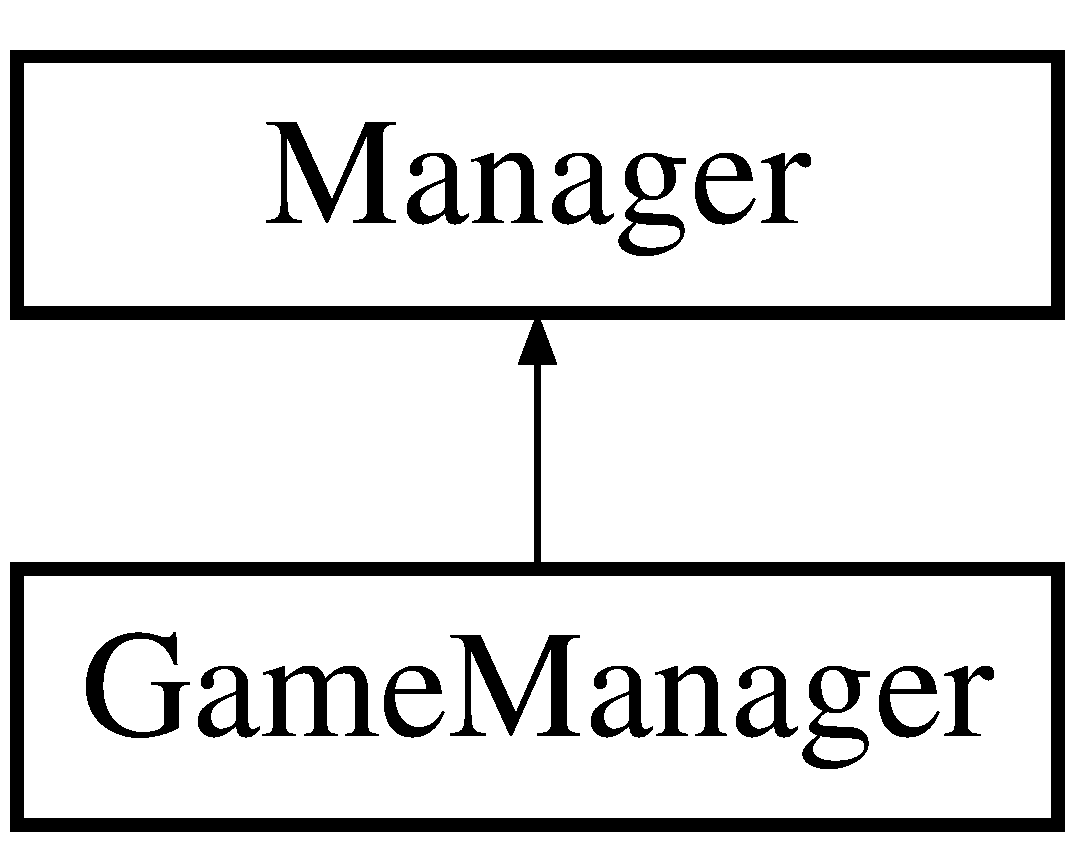
\includegraphics[height=2.000000cm]{class_game_manager}
\end{center}
\end{figure}
\subsection*{Public Member Functions}
\begin{DoxyCompactItemize}
\item 
int \hyperlink{class_game_manager_a6626dd9f245039379b3416e2a28bb71c}{start\+Up} ()
\item 
void \hyperlink{class_game_manager_a6cbd6266472fb9c0b08a4c2f7f8813af}{shut\+Down} ()
\item 
void \hyperlink{class_game_manager_a3d5daf583c259edaf29c4b66ac20e480}{run} (unsigned int frame\+Time=D\+E\+F\+A\+U\+L\+T\+\_\+\+F\+R\+A\+M\+E\+\_\+\+T\+I\+M\+E)
\item 
void \hyperlink{class_game_manager_a18b1e6e63207f3fb71b4c3ce771bf704}{set\+Game\+Over} (bool game\+Over=true)
\item 
bool \hyperlink{class_game_manager_a5025aec4010d2c30631c0be20e94efee}{is\+Game\+Over} () const 
\item 
unsigned int \hyperlink{class_game_manager_a40be71508d2e97a080c6eb1acf5b8624}{get\+Frame\+Time} () const 
\item 
\hypertarget{class_game_manager_a821bef9440389f456a296a145ad30884}{unsigned int {\bfseries get\+Tick\+Count} () const }\label{class_game_manager_a821bef9440389f456a296a145ad30884}

\end{DoxyCompactItemize}
\subsection*{Static Public Member Functions}
\begin{DoxyCompactItemize}
\item 
static \hyperlink{class_game_manager}{Game\+Manager} \& \hyperlink{class_game_manager_a62c0bd2e38276cc3805fb38a85890d42}{get\+Instance} ()
\end{DoxyCompactItemize}


\subsection{Detailed Description}
Handles game management 

\subsection{Member Function Documentation}
\hypertarget{class_game_manager_a40be71508d2e97a080c6eb1acf5b8624}{\index{Game\+Manager@{Game\+Manager}!get\+Frame\+Time@{get\+Frame\+Time}}
\index{get\+Frame\+Time@{get\+Frame\+Time}!Game\+Manager@{Game\+Manager}}
\subsubsection[{get\+Frame\+Time}]{\setlength{\rightskip}{0pt plus 5cm}unsigned int Game\+Manager\+::get\+Frame\+Time (
\begin{DoxyParamCaption}
{}
\end{DoxyParamCaption}
) const}}\label{class_game_manager_a40be71508d2e97a080c6eb1acf5b8624}
Gets the time between frames \begin{DoxyReturn}{Returns}
An unsigned integer showing the time between frames in milliseconds 
\end{DoxyReturn}
\hypertarget{class_game_manager_a62c0bd2e38276cc3805fb38a85890d42}{\index{Game\+Manager@{Game\+Manager}!get\+Instance@{get\+Instance}}
\index{get\+Instance@{get\+Instance}!Game\+Manager@{Game\+Manager}}
\subsubsection[{get\+Instance}]{\setlength{\rightskip}{0pt plus 5cm}{\bf Game\+Manager} \& Game\+Manager\+::get\+Instance (
\begin{DoxyParamCaption}
{}
\end{DoxyParamCaption}
)\hspace{0.3cm}{\ttfamily [static]}}}\label{class_game_manager_a62c0bd2e38276cc3805fb38a85890d42}
Gets the game manager instance \begin{DoxyReturn}{Returns}
A reference to the game manager instance 
\end{DoxyReturn}
\hypertarget{class_game_manager_a5025aec4010d2c30631c0be20e94efee}{\index{Game\+Manager@{Game\+Manager}!is\+Game\+Over@{is\+Game\+Over}}
\index{is\+Game\+Over@{is\+Game\+Over}!Game\+Manager@{Game\+Manager}}
\subsubsection[{is\+Game\+Over}]{\setlength{\rightskip}{0pt plus 5cm}bool Game\+Manager\+::is\+Game\+Over (
\begin{DoxyParamCaption}
{}
\end{DoxyParamCaption}
) const}}\label{class_game_manager_a5025aec4010d2c30631c0be20e94efee}
Gets the value of the game over flag \begin{DoxyReturn}{Returns}
The value of the game over flag 
\end{DoxyReturn}
\hypertarget{class_game_manager_a3d5daf583c259edaf29c4b66ac20e480}{\index{Game\+Manager@{Game\+Manager}!run@{run}}
\index{run@{run}!Game\+Manager@{Game\+Manager}}
\subsubsection[{run}]{\setlength{\rightskip}{0pt plus 5cm}void Game\+Manager\+::run (
\begin{DoxyParamCaption}
\item[{unsigned int}]{frame\+Time = {\ttfamily DEFAULT\+\_\+FRAME\+\_\+TIME}}
\end{DoxyParamCaption}
)}}\label{class_game_manager_a3d5daf583c259edaf29c4b66ac20e480}
Runs the main game loop 
\begin{DoxyParams}{Parameters}
{\em frame\+Time} & The fixed time to have between frames \\
\hline
\end{DoxyParams}
\hypertarget{class_game_manager_a18b1e6e63207f3fb71b4c3ce771bf704}{\index{Game\+Manager@{Game\+Manager}!set\+Game\+Over@{set\+Game\+Over}}
\index{set\+Game\+Over@{set\+Game\+Over}!Game\+Manager@{Game\+Manager}}
\subsubsection[{set\+Game\+Over}]{\setlength{\rightskip}{0pt plus 5cm}void Game\+Manager\+::set\+Game\+Over (
\begin{DoxyParamCaption}
\item[{bool}]{game\+Over = {\ttfamily true}}
\end{DoxyParamCaption}
)}}\label{class_game_manager_a18b1e6e63207f3fb71b4c3ce771bf704}
Set the game over flag in the game 
\begin{DoxyParams}{Parameters}
{\em game\+Over} & The value to set the game over flag to \\
\hline
\end{DoxyParams}
\hypertarget{class_game_manager_a6cbd6266472fb9c0b08a4c2f7f8813af}{\index{Game\+Manager@{Game\+Manager}!shut\+Down@{shut\+Down}}
\index{shut\+Down@{shut\+Down}!Game\+Manager@{Game\+Manager}}
\subsubsection[{shut\+Down}]{\setlength{\rightskip}{0pt plus 5cm}void Game\+Manager\+::shut\+Down (
\begin{DoxyParamCaption}
{}
\end{DoxyParamCaption}
)\hspace{0.3cm}{\ttfamily [virtual]}}}\label{class_game_manager_a6cbd6266472fb9c0b08a4c2f7f8813af}
Called when the game manager shuts down 

Reimplemented from \hyperlink{class_manager_a09f0aaf6012be52b75a12fac25370f61}{Manager}.

\hypertarget{class_game_manager_a6626dd9f245039379b3416e2a28bb71c}{\index{Game\+Manager@{Game\+Manager}!start\+Up@{start\+Up}}
\index{start\+Up@{start\+Up}!Game\+Manager@{Game\+Manager}}
\subsubsection[{start\+Up}]{\setlength{\rightskip}{0pt plus 5cm}int Game\+Manager\+::start\+Up (
\begin{DoxyParamCaption}
{}
\end{DoxyParamCaption}
)\hspace{0.3cm}{\ttfamily [virtual]}}}\label{class_game_manager_a6626dd9f245039379b3416e2a28bb71c}
Called when the game manager is started \begin{DoxyReturn}{Returns}
0 when no errors occur, $<$ 0 when an error does occur 
\end{DoxyReturn}


Reimplemented from \hyperlink{class_manager_a2a0f0d6810a5a051afd707d83ff1ff36}{Manager}.



The documentation for this class was generated from the following files\+:\begin{DoxyCompactItemize}
\item 
F\+:/\+Users/\+Benny/git/\+I\+M\+G\+D3000/\+I\+M\+G\+D3000\+Proj3/include/Game\+Manager.\+h\item 
F\+:/\+Users/\+Benny/git/\+I\+M\+G\+D3000/\+I\+M\+G\+D3000\+Proj3/lib/src/\+Game/Game\+Manager.\+cpp\end{DoxyCompactItemize}

\hypertarget{class_graphics_manager}{\section{Graphics\+Manager Class Reference}
\label{class_graphics_manager}\index{Graphics\+Manager@{Graphics\+Manager}}
}


{\ttfamily \#include $<$Graphics\+Manager.\+h$>$}

Inheritance diagram for Graphics\+Manager\+:\begin{figure}[H]
\begin{center}
\leavevmode
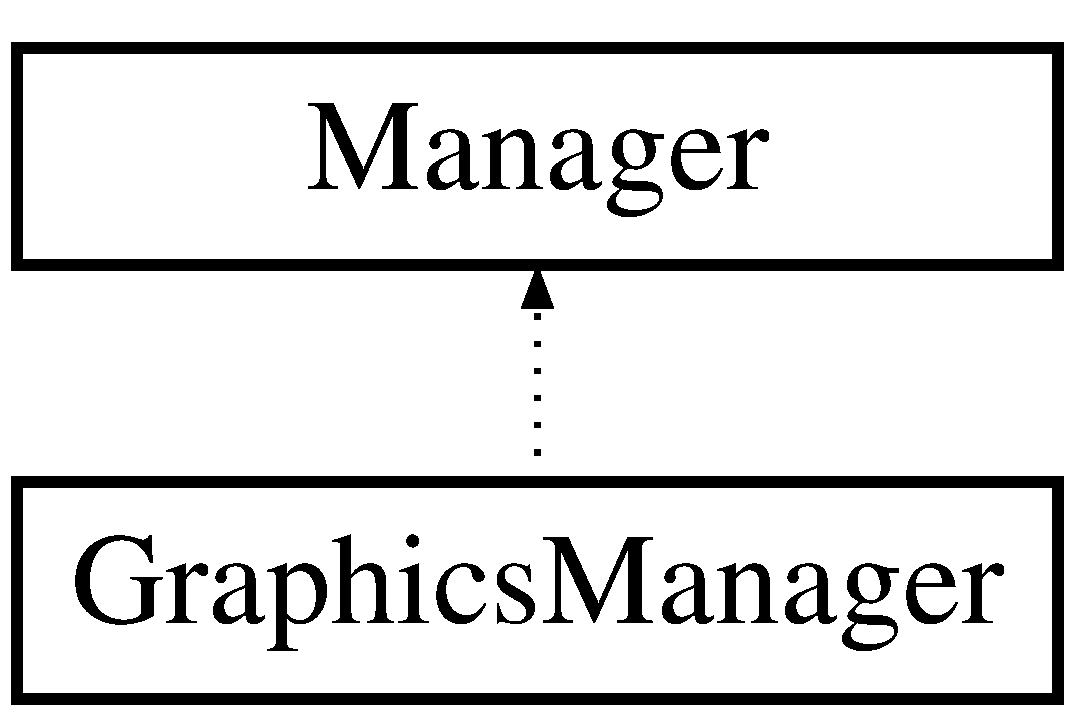
\includegraphics[height=2.000000cm]{class_graphics_manager}
\end{center}
\end{figure}
\subsection*{Public Member Functions}
\begin{DoxyCompactItemize}
\item 
int \hyperlink{class_graphics_manager_ac1961e1b4985a41a6eb233736d5d3191}{start\+Up} ()
\item 
void \hyperlink{class_graphics_manager_a5d850ef5d3a6792eb270fa22b784b3e6}{shut\+Down} ()
\item 
int \hyperlink{class_graphics_manager_a18954a6304591268760d2eab5804d7b3}{swap\+Buffer} (bool clear=true)
\item 
int \hyperlink{class_graphics_manager_a4d727210ad9f36755f961f1ef95a9edb}{get\+Horizontal} () const 
\item 
int \hyperlink{class_graphics_manager_a8285df9ae37927930fac787293041517}{get\+Vertical} () const 
\item 
int \hyperlink{class_graphics_manager_a99cd53145eebabc3cb707bb8717a8529}{draw\+Ch} (\hyperlink{class_i_vector}{I\+Vector} world\+Pos, char c, int color=D\+F\+\_\+\+D\+E\+F\+A\+U\+L\+T\+\_\+\+C\+O\+L\+O\+R) const 
\item 
int \hyperlink{class_graphics_manager_ab7925ff75e907e644199ed042f4d35e1}{draw\+String} (\hyperlink{class_i_vector}{I\+Vector} world\+Pos, Justification justification, string str, int color=D\+F\+\_\+\+D\+E\+F\+A\+U\+L\+T\+\_\+\+C\+O\+L\+O\+R) const 
\item 
int \hyperlink{class_graphics_manager_a46fdb7da074537ca39b8b0e91ec9f95a}{draw\+Frame} (\hyperlink{class_i_vector}{I\+Vector} world\+Pos, const \hyperlink{class_frame}{Frame} $\ast$frame, bool centered, int color=D\+F\+\_\+\+D\+E\+F\+A\+U\+L\+T\+\_\+\+C\+O\+L\+O\+R) const 
\item 
W\+I\+N\+D\+O\+W $\ast$ \hyperlink{class_graphics_manager_a5387f69913132a6e572fa1018961640f}{get\+Back\+Buffer} () const 
\item 
W\+I\+N\+D\+O\+W $\ast$ \hyperlink{class_graphics_manager_a0c6b0d00061ca962eeefbe813879ceb4}{get\+Front\+Buffer} () const 
\end{DoxyCompactItemize}
\subsection*{Static Public Member Functions}
\begin{DoxyCompactItemize}
\item 
static \hyperlink{class_graphics_manager}{Graphics\+Manager} \& \hyperlink{class_graphics_manager_acd82b9108141b60d9f4b38d104b8165a}{get\+Instance} ()
\end{DoxyCompactItemize}


\subsection{Detailed Description}
Manages drawing and rendering to the screen 

\subsection{Member Function Documentation}
\hypertarget{class_graphics_manager_a99cd53145eebabc3cb707bb8717a8529}{\index{Graphics\+Manager@{Graphics\+Manager}!draw\+Ch@{draw\+Ch}}
\index{draw\+Ch@{draw\+Ch}!Graphics\+Manager@{Graphics\+Manager}}
\subsubsection[{draw\+Ch}]{\setlength{\rightskip}{0pt plus 5cm}int Graphics\+Manager\+::draw\+Ch (
\begin{DoxyParamCaption}
\item[{{\bf I\+Vector}}]{world\+Pos, }
\item[{char}]{c, }
\item[{int}]{color = {\ttfamily DF\+\_\+DEFAULT\+\_\+COLOR}}
\end{DoxyParamCaption}
) const}}\label{class_graphics_manager_a99cd53145eebabc3cb707bb8717a8529}
Draws a character at the world position 
\begin{DoxyParams}{Parameters}
{\em world\+Pos} & The world position to draw the character at \\
\hline
{\em c} & The character to draw \\
\hline
{\em color} & The color to draw the character \\
\hline
\end{DoxyParams}
\begin{DoxyReturn}{Returns}
0 if ok, -\/1 if not 
\end{DoxyReturn}
\hypertarget{class_graphics_manager_a46fdb7da074537ca39b8b0e91ec9f95a}{\index{Graphics\+Manager@{Graphics\+Manager}!draw\+Frame@{draw\+Frame}}
\index{draw\+Frame@{draw\+Frame}!Graphics\+Manager@{Graphics\+Manager}}
\subsubsection[{draw\+Frame}]{\setlength{\rightskip}{0pt plus 5cm}int Graphics\+Manager\+::draw\+Frame (
\begin{DoxyParamCaption}
\item[{{\bf I\+Vector}}]{world\+Pos, }
\item[{const {\bf Frame} $\ast$}]{frame, }
\item[{bool}]{centered, }
\item[{int}]{color = {\ttfamily DF\+\_\+DEFAULT\+\_\+COLOR}}
\end{DoxyParamCaption}
) const}}\label{class_graphics_manager_a46fdb7da074537ca39b8b0e91ec9f95a}
Draws a frame of characters 
\begin{DoxyParams}{Parameters}
{\em world\+Pos} & The world position to draw the frame at \\
\hline
{\em frame} & The frame to draw \\
\hline
{\em centered} & If true, then we should consider the draw point the center of the frame \\
\hline
{\em color} & The color to draw the frame with \\
\hline
\end{DoxyParams}
\begin{DoxyReturn}{Returns}
0 on ok , -\/1 on fail 
\end{DoxyReturn}
\hypertarget{class_graphics_manager_ab7925ff75e907e644199ed042f4d35e1}{\index{Graphics\+Manager@{Graphics\+Manager}!draw\+String@{draw\+String}}
\index{draw\+String@{draw\+String}!Graphics\+Manager@{Graphics\+Manager}}
\subsubsection[{draw\+String}]{\setlength{\rightskip}{0pt plus 5cm}int Graphics\+Manager\+::draw\+String (
\begin{DoxyParamCaption}
\item[{{\bf I\+Vector}}]{world\+Pos, }
\item[{Justification}]{justification, }
\item[{string}]{str, }
\item[{int}]{color = {\ttfamily DF\+\_\+DEFAULT\+\_\+COLOR}}
\end{DoxyParamCaption}
) const}}\label{class_graphics_manager_ab7925ff75e907e644199ed042f4d35e1}
Draws a string at the world position 
\begin{DoxyParams}{Parameters}
{\em world\+Pos} & The world position to draw the string at \\
\hline
{\em justification} & The justification to draw the string at \\
\hline
{\em str} & The string to draw \\
\hline
{\em color} & The color to draw the string with \\
\hline
\end{DoxyParams}
\begin{DoxyReturn}{Returns}
0 on ok, -\/1 to on fail 
\end{DoxyReturn}
\hypertarget{class_graphics_manager_a5387f69913132a6e572fa1018961640f}{\index{Graphics\+Manager@{Graphics\+Manager}!get\+Back\+Buffer@{get\+Back\+Buffer}}
\index{get\+Back\+Buffer@{get\+Back\+Buffer}!Graphics\+Manager@{Graphics\+Manager}}
\subsubsection[{get\+Back\+Buffer}]{\setlength{\rightskip}{0pt plus 5cm}W\+I\+N\+D\+O\+W $\ast$ Graphics\+Manager\+::get\+Back\+Buffer (
\begin{DoxyParamCaption}
{}
\end{DoxyParamCaption}
) const}}\label{class_graphics_manager_a5387f69913132a6e572fa1018961640f}
Gets the current buffer we are rendering to \begin{DoxyReturn}{Returns}
A pointer to the back buffer 
\end{DoxyReturn}
\hypertarget{class_graphics_manager_a0c6b0d00061ca962eeefbe813879ceb4}{\index{Graphics\+Manager@{Graphics\+Manager}!get\+Front\+Buffer@{get\+Front\+Buffer}}
\index{get\+Front\+Buffer@{get\+Front\+Buffer}!Graphics\+Manager@{Graphics\+Manager}}
\subsubsection[{get\+Front\+Buffer}]{\setlength{\rightskip}{0pt plus 5cm}W\+I\+N\+D\+O\+W $\ast$ Graphics\+Manager\+::get\+Front\+Buffer (
\begin{DoxyParamCaption}
{}
\end{DoxyParamCaption}
) const}}\label{class_graphics_manager_a0c6b0d00061ca962eeefbe813879ceb4}
Gets the current buffer we are displaying \begin{DoxyReturn}{Returns}
A pointer to the front buffer 
\end{DoxyReturn}
\hypertarget{class_graphics_manager_a4d727210ad9f36755f961f1ef95a9edb}{\index{Graphics\+Manager@{Graphics\+Manager}!get\+Horizontal@{get\+Horizontal}}
\index{get\+Horizontal@{get\+Horizontal}!Graphics\+Manager@{Graphics\+Manager}}
\subsubsection[{get\+Horizontal}]{\setlength{\rightskip}{0pt plus 5cm}int Graphics\+Manager\+::get\+Horizontal (
\begin{DoxyParamCaption}
{}
\end{DoxyParamCaption}
) const}}\label{class_graphics_manager_a4d727210ad9f36755f961f1ef95a9edb}
Gets the horizontal size of the terminal in characters \begin{DoxyReturn}{Returns}
An integer showing how many characters across the terminal is 
\end{DoxyReturn}
\hypertarget{class_graphics_manager_acd82b9108141b60d9f4b38d104b8165a}{\index{Graphics\+Manager@{Graphics\+Manager}!get\+Instance@{get\+Instance}}
\index{get\+Instance@{get\+Instance}!Graphics\+Manager@{Graphics\+Manager}}
\subsubsection[{get\+Instance}]{\setlength{\rightskip}{0pt plus 5cm}{\bf Graphics\+Manager} \& Graphics\+Manager\+::get\+Instance (
\begin{DoxyParamCaption}
{}
\end{DoxyParamCaption}
)\hspace{0.3cm}{\ttfamily [static]}}}\label{class_graphics_manager_acd82b9108141b60d9f4b38d104b8165a}
Get the graphics manager instance \begin{DoxyReturn}{Returns}
A reference to the graphics manager instance 
\end{DoxyReturn}
\hypertarget{class_graphics_manager_a8285df9ae37927930fac787293041517}{\index{Graphics\+Manager@{Graphics\+Manager}!get\+Vertical@{get\+Vertical}}
\index{get\+Vertical@{get\+Vertical}!Graphics\+Manager@{Graphics\+Manager}}
\subsubsection[{get\+Vertical}]{\setlength{\rightskip}{0pt plus 5cm}int Graphics\+Manager\+::get\+Vertical (
\begin{DoxyParamCaption}
{}
\end{DoxyParamCaption}
) const}}\label{class_graphics_manager_a8285df9ae37927930fac787293041517}
Gets the vertical size of the terminal in characters \begin{DoxyReturn}{Returns}
An integer showing how many characters across the terminal is 
\end{DoxyReturn}
\hypertarget{class_graphics_manager_a5d850ef5d3a6792eb270fa22b784b3e6}{\index{Graphics\+Manager@{Graphics\+Manager}!shut\+Down@{shut\+Down}}
\index{shut\+Down@{shut\+Down}!Graphics\+Manager@{Graphics\+Manager}}
\subsubsection[{shut\+Down}]{\setlength{\rightskip}{0pt plus 5cm}void Graphics\+Manager\+::shut\+Down (
\begin{DoxyParamCaption}
{}
\end{DoxyParamCaption}
)\hspace{0.3cm}{\ttfamily [virtual]}}}\label{class_graphics_manager_a5d850ef5d3a6792eb270fa22b784b3e6}
Called when the graphics manager is shutdown 

Reimplemented from \hyperlink{class_manager_a09f0aaf6012be52b75a12fac25370f61}{Manager}.

\hypertarget{class_graphics_manager_ac1961e1b4985a41a6eb233736d5d3191}{\index{Graphics\+Manager@{Graphics\+Manager}!start\+Up@{start\+Up}}
\index{start\+Up@{start\+Up}!Graphics\+Manager@{Graphics\+Manager}}
\subsubsection[{start\+Up}]{\setlength{\rightskip}{0pt plus 5cm}int Graphics\+Manager\+::start\+Up (
\begin{DoxyParamCaption}
{}
\end{DoxyParamCaption}
)\hspace{0.3cm}{\ttfamily [virtual]}}}\label{class_graphics_manager_ac1961e1b4985a41a6eb233736d5d3191}
Called when the graphics manager is started \begin{DoxyReturn}{Returns}
0 if the graphics manager was started, otherwise returns $<$ 0 
\end{DoxyReturn}


Reimplemented from \hyperlink{class_manager_a2a0f0d6810a5a051afd707d83ff1ff36}{Manager}.

\hypertarget{class_graphics_manager_a18954a6304591268760d2eab5804d7b3}{\index{Graphics\+Manager@{Graphics\+Manager}!swap\+Buffer@{swap\+Buffer}}
\index{swap\+Buffer@{swap\+Buffer}!Graphics\+Manager@{Graphics\+Manager}}
\subsubsection[{swap\+Buffer}]{\setlength{\rightskip}{0pt plus 5cm}int Graphics\+Manager\+::swap\+Buffer (
\begin{DoxyParamCaption}
\item[{bool}]{clear = {\ttfamily true}}
\end{DoxyParamCaption}
)}}\label{class_graphics_manager_a18954a6304591268760d2eab5804d7b3}
Swaps the front and back buffer 
\begin{DoxyParams}{Parameters}
{\em clear} & If true, clears the new back buffer \\
\hline
\end{DoxyParams}
\begin{DoxyReturn}{Returns}
1 when the swap worked, -\/1 if not 
\end{DoxyReturn}


The documentation for this class was generated from the following files\+:\begin{DoxyCompactItemize}
\item 
F\+:/\+Users/\+Benny/git/\+I\+M\+G\+D3000/\+I\+M\+G\+D3000\+Proj3/include/Graphics\+Manager.\+h\item 
F\+:/\+Users/\+Benny/git/\+I\+M\+G\+D3000/\+I\+M\+G\+D3000\+Proj3/lib/src/\+Rendering/Graphics\+Manager.\+cpp\end{DoxyCompactItemize}

\hypertarget{class_hash_table}{\section{Hash\+Table Class Reference}
\label{class_hash_table}\index{Hash\+Table@{Hash\+Table}}
}


{\ttfamily \#include $<$Hash\+Table.\+h$>$}

\subsection*{Public Member Functions}
\begin{DoxyCompactItemize}
\item 
\hyperlink{class_hash_table_a41c9ebff33f0f4b9583b087953962f87}{Hash\+Table} (size\+\_\+t bucket\+Count=D\+E\+F\+A\+U\+L\+T\+\_\+\+B\+U\+C\+K\+E\+T\+\_\+\+C\+O\+U\+N\+T)
\item 
void $\ast$ \hyperlink{class_hash_table_a86f22156f16fa378f34545cee2d6d305}{set} (string key, void $\ast$value)
\item 
void $\ast$ \hyperlink{class_hash_table_a475da9ba22ac4e91f893213fa38a8692}{remove} (string key)
\item 
bool \hyperlink{class_hash_table_a5acad447b9f94de98192bb7fa30f56c5}{contains} (string key)
\item 
void $\ast$ \hyperlink{class_hash_table_af11799eb3e8403eb24f8e1ebfa514981}{get} (string key)
\end{DoxyCompactItemize}


\subsection{Detailed Description}
Provides a string to ptr hashtable By using a ptr like a base data type you could in theory store any 4-\/byte or under data 

\subsection{Constructor \& Destructor Documentation}
\hypertarget{class_hash_table_a41c9ebff33f0f4b9583b087953962f87}{\index{Hash\+Table@{Hash\+Table}!Hash\+Table@{Hash\+Table}}
\index{Hash\+Table@{Hash\+Table}!Hash\+Table@{Hash\+Table}}
\subsubsection[{Hash\+Table}]{\setlength{\rightskip}{0pt plus 5cm}Hash\+Table\+::\+Hash\+Table (
\begin{DoxyParamCaption}
\item[{size\+\_\+t}]{bucket\+Count = {\ttfamily DEFAULT\+\_\+BUCKET\+\_\+COUNT}}
\end{DoxyParamCaption}
)}}\label{class_hash_table_a41c9ebff33f0f4b9583b087953962f87}
Creates a new hashtable 
\begin{DoxyParams}{Parameters}
{\em bucket\+Count} & The number of buckets to create to store info in \\
\hline
\end{DoxyParams}


\subsection{Member Function Documentation}
\hypertarget{class_hash_table_a5acad447b9f94de98192bb7fa30f56c5}{\index{Hash\+Table@{Hash\+Table}!contains@{contains}}
\index{contains@{contains}!Hash\+Table@{Hash\+Table}}
\subsubsection[{contains}]{\setlength{\rightskip}{0pt plus 5cm}bool Hash\+Table\+::contains (
\begin{DoxyParamCaption}
\item[{string}]{key}
\end{DoxyParamCaption}
)}}\label{class_hash_table_a5acad447b9f94de98192bb7fa30f56c5}
Checks to see if the hashtable contains a key 
\begin{DoxyParams}{Parameters}
{\em key} & The key to check for \\
\hline
\end{DoxyParams}
\begin{DoxyReturn}{Returns}
True if the key exists, false otherwise 
\end{DoxyReturn}
\hypertarget{class_hash_table_af11799eb3e8403eb24f8e1ebfa514981}{\index{Hash\+Table@{Hash\+Table}!get@{get}}
\index{get@{get}!Hash\+Table@{Hash\+Table}}
\subsubsection[{get}]{\setlength{\rightskip}{0pt plus 5cm}void $\ast$ Hash\+Table\+::get (
\begin{DoxyParamCaption}
\item[{string}]{key}
\end{DoxyParamCaption}
)}}\label{class_hash_table_af11799eb3e8403eb24f8e1ebfa514981}
Gets the value stored at the key 
\begin{DoxyParams}{Parameters}
{\em key} & The key to get the value at \\
\hline
\end{DoxyParams}
\begin{DoxyReturn}{Returns}
The ptr value at that key, or N\+U\+L\+L if the key could not be found 
\end{DoxyReturn}
\hypertarget{class_hash_table_a475da9ba22ac4e91f893213fa38a8692}{\index{Hash\+Table@{Hash\+Table}!remove@{remove}}
\index{remove@{remove}!Hash\+Table@{Hash\+Table}}
\subsubsection[{remove}]{\setlength{\rightskip}{0pt plus 5cm}void $\ast$ Hash\+Table\+::remove (
\begin{DoxyParamCaption}
\item[{string}]{key}
\end{DoxyParamCaption}
)}}\label{class_hash_table_a475da9ba22ac4e91f893213fa38a8692}
Removes a key from the hashtable 
\begin{DoxyParams}{Parameters}
{\em key} & They key to remove \\
\hline
\end{DoxyParams}
\begin{DoxyReturn}{Returns}
The value that was at that key, or N\+U\+L\+L if the key wasn't found 
\end{DoxyReturn}
\hypertarget{class_hash_table_a86f22156f16fa378f34545cee2d6d305}{\index{Hash\+Table@{Hash\+Table}!set@{set}}
\index{set@{set}!Hash\+Table@{Hash\+Table}}
\subsubsection[{set}]{\setlength{\rightskip}{0pt plus 5cm}void $\ast$ Hash\+Table\+::set (
\begin{DoxyParamCaption}
\item[{string}]{key, }
\item[{void $\ast$}]{value}
\end{DoxyParamCaption}
)}}\label{class_hash_table_a86f22156f16fa378f34545cee2d6d305}
Sets the value to store at a key inside the hash table 
\begin{DoxyParams}{Parameters}
{\em key} & The key to use \\
\hline
{\em value} & The value to store at that key \\
\hline
\end{DoxyParams}
\begin{DoxyReturn}{Returns}
The value that was at that key, or if its a new key then N\+U\+L\+L 
\end{DoxyReturn}


The documentation for this class was generated from the following files\+:\begin{DoxyCompactItemize}
\item 
F\+:/\+Users/\+Benny/git/\+I\+M\+G\+D3000/\+I\+M\+G\+D3000\+Proj3/include/Hash\+Table.\+h\item 
F\+:/\+Users/\+Benny/git/\+I\+M\+G\+D3000/\+I\+M\+G\+D3000\+Proj3/lib/src/\+Core/Hash\+Table.\+cpp\end{DoxyCompactItemize}

\hypertarget{class_input_manager}{\section{Input\+Manager Class Reference}
\label{class_input_manager}\index{Input\+Manager@{Input\+Manager}}
}


{\ttfamily \#include $<$Input\+Manager.\+h$>$}

Inheritance diagram for Input\+Manager\+:\begin{figure}[H]
\begin{center}
\leavevmode
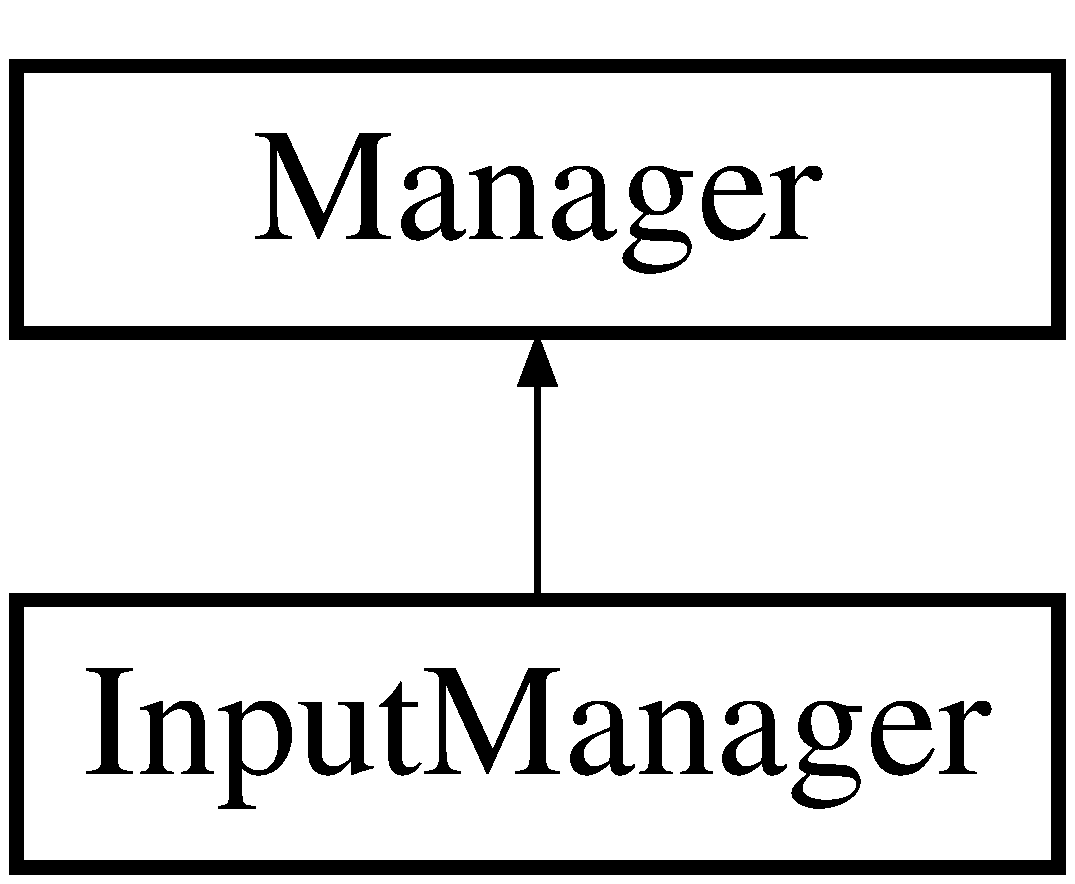
\includegraphics[height=2.000000cm]{class_input_manager}
\end{center}
\end{figure}
\subsection*{Public Member Functions}
\begin{DoxyCompactItemize}
\item 
int \hyperlink{class_input_manager_a210997e45748bae7d0901ac3ede788c6}{start\+Up} ()
\item 
void \hyperlink{class_input_manager_ad9ae425dbb849fda4616484e7156600e}{shut\+Down} ()
\item 
void \hyperlink{class_input_manager_a3701626b38fab73b47561fa961a2739e}{get\+Input} ()
\end{DoxyCompactItemize}
\subsection*{Static Public Member Functions}
\begin{DoxyCompactItemize}
\item 
static \hyperlink{class_input_manager}{Input\+Manager} \& \hyperlink{class_input_manager_a4e1058b89c07e2f3ec1097b843c19fc8}{get\+Instance} ()
\end{DoxyCompactItemize}


\subsection{Detailed Description}
A singleton class that handles ionput 

\subsection{Member Function Documentation}
\hypertarget{class_input_manager_a3701626b38fab73b47561fa961a2739e}{\index{Input\+Manager@{Input\+Manager}!get\+Input@{get\+Input}}
\index{get\+Input@{get\+Input}!Input\+Manager@{Input\+Manager}}
\subsubsection[{get\+Input}]{\setlength{\rightskip}{0pt plus 5cm}void Input\+Manager\+::get\+Input (
\begin{DoxyParamCaption}
{}
\end{DoxyParamCaption}
)}}\label{class_input_manager_a3701626b38fab73b47561fa961a2739e}
Called once per frame to check the input device for events \hypertarget{class_input_manager_a4e1058b89c07e2f3ec1097b843c19fc8}{\index{Input\+Manager@{Input\+Manager}!get\+Instance@{get\+Instance}}
\index{get\+Instance@{get\+Instance}!Input\+Manager@{Input\+Manager}}
\subsubsection[{get\+Instance}]{\setlength{\rightskip}{0pt plus 5cm}{\bf Input\+Manager} \& Input\+Manager\+::get\+Instance (
\begin{DoxyParamCaption}
{}
\end{DoxyParamCaption}
)\hspace{0.3cm}{\ttfamily [static]}}}\label{class_input_manager_a4e1058b89c07e2f3ec1097b843c19fc8}
Get the static instance of this object \begin{DoxyReturn}{Returns}
A reference to the input manager 
\end{DoxyReturn}
\hypertarget{class_input_manager_ad9ae425dbb849fda4616484e7156600e}{\index{Input\+Manager@{Input\+Manager}!shut\+Down@{shut\+Down}}
\index{shut\+Down@{shut\+Down}!Input\+Manager@{Input\+Manager}}
\subsubsection[{shut\+Down}]{\setlength{\rightskip}{0pt plus 5cm}void Input\+Manager\+::shut\+Down (
\begin{DoxyParamCaption}
{}
\end{DoxyParamCaption}
)\hspace{0.3cm}{\ttfamily [virtual]}}}\label{class_input_manager_ad9ae425dbb849fda4616484e7156600e}
Called when the input manager is shutdown 

Reimplemented from \hyperlink{class_manager_a09f0aaf6012be52b75a12fac25370f61}{Manager}.

\hypertarget{class_input_manager_a210997e45748bae7d0901ac3ede788c6}{\index{Input\+Manager@{Input\+Manager}!start\+Up@{start\+Up}}
\index{start\+Up@{start\+Up}!Input\+Manager@{Input\+Manager}}
\subsubsection[{start\+Up}]{\setlength{\rightskip}{0pt plus 5cm}int Input\+Manager\+::start\+Up (
\begin{DoxyParamCaption}
{}
\end{DoxyParamCaption}
)\hspace{0.3cm}{\ttfamily [virtual]}}}\label{class_input_manager_a210997e45748bae7d0901ac3ede788c6}
Called when the input manager is started \begin{DoxyReturn}{Returns}
0 if ok, otherwise -\/1 
\end{DoxyReturn}


Reimplemented from \hyperlink{class_manager_a2a0f0d6810a5a051afd707d83ff1ff36}{Manager}.



The documentation for this class was generated from the following files\+:\begin{DoxyCompactItemize}
\item 
F\+:/\+Users/\+Benny/git/\+I\+M\+G\+D3000/\+I\+M\+G\+D3000\+Proj3/include/Input\+Manager.\+h\item 
F\+:/\+Users/\+Benny/git/\+I\+M\+G\+D3000/\+I\+M\+G\+D3000\+Proj3/lib/src/\+Input/Input\+Manager.\+cpp\end{DoxyCompactItemize}

\hypertarget{class_i_vector}{\section{I\+Vector Class Reference}
\label{class_i_vector}\index{I\+Vector@{I\+Vector}}
}


{\ttfamily \#include $<$I\+Vector.\+h$>$}

\subsection*{Public Member Functions}
\begin{DoxyCompactItemize}
\item 
\hyperlink{class_i_vector_adeabc4b0f4932cda5b4c8040da2dfc62}{I\+Vector} (int x, int y)
\item 
\hyperlink{class_i_vector_a28fc0ca78c5f7d7b241a5225396f8da5}{I\+Vector} (\hyperlink{class_f_vector}{F\+Vector} \&fvec)
\item 
void \hyperlink{class_i_vector_a6dce9a639a609e28bb0f814c1e2cf82e}{set} (int x, int y)
\item 
void \hyperlink{class_i_vector_a2256218449a4ff6df57cdb41fb09877f}{set\+X} (int x)
\item 
void \hyperlink{class_i_vector_a7e70cc0470077112cac352086f8ab500}{set\+Y} (int y)
\item 
int \hyperlink{class_i_vector_a255464399d9901bc2efc3b197b380b0e}{get\+X} () const 
\item 
int \hyperlink{class_i_vector_a2bf064a07ecf6912cf9e7bd44ad12073}{get\+Y} () const 
\item 
\hyperlink{class_i_vector}{I\+Vector} \hyperlink{class_i_vector_a6700c03ecc1e857a78b2066f39a018d5}{operator+} (const \hyperlink{class_i_vector}{I\+Vector} \&b) const 
\item 
\hyperlink{class_i_vector}{I\+Vector} \hyperlink{class_i_vector_a275b2a8da268c5df8f74f36c950c1236}{operator-\/} (const \hyperlink{class_i_vector}{I\+Vector} \&b) const 
\item 
\hyperlink{class_i_vector}{I\+Vector} \hyperlink{class_i_vector_a0115772afbf7ab7e986881353539759d}{operator-\/} () const 
\item 
bool \hyperlink{class_i_vector_a8cf7d091e70efc188b3f04e1aa9ab439}{operator==} (const \hyperlink{class_i_vector}{I\+Vector} \&b) const 
\item 
bool \hyperlink{class_i_vector_ab29fc9f9cd118682d086110f30273cf5}{operator!=} (const \hyperlink{class_i_vector}{I\+Vector} \&b) const 
\end{DoxyCompactItemize}


\subsection{Detailed Description}
A 2d integer vector 

\subsection{Constructor \& Destructor Documentation}
\hypertarget{class_i_vector_adeabc4b0f4932cda5b4c8040da2dfc62}{\index{I\+Vector@{I\+Vector}!I\+Vector@{I\+Vector}}
\index{I\+Vector@{I\+Vector}!I\+Vector@{I\+Vector}}
\subsubsection[{I\+Vector}]{\setlength{\rightskip}{0pt plus 5cm}I\+Vector\+::\+I\+Vector (
\begin{DoxyParamCaption}
\item[{int}]{x, }
\item[{int}]{y}
\end{DoxyParamCaption}
)}}\label{class_i_vector_adeabc4b0f4932cda5b4c8040da2dfc62}
Creates a new \hyperlink{class_i_vector}{I\+Vector} 
\begin{DoxyParams}{Parameters}
{\em x} & The x coordinate of the \hyperlink{class_i_vector}{I\+Vector} \\
\hline
{\em y} & The y coordinate of the \hyperlink{class_i_vector}{I\+Vector} \\
\hline
\end{DoxyParams}
\hypertarget{class_i_vector_a28fc0ca78c5f7d7b241a5225396f8da5}{\index{I\+Vector@{I\+Vector}!I\+Vector@{I\+Vector}}
\index{I\+Vector@{I\+Vector}!I\+Vector@{I\+Vector}}
\subsubsection[{I\+Vector}]{\setlength{\rightskip}{0pt plus 5cm}I\+Vector\+::\+I\+Vector (
\begin{DoxyParamCaption}
\item[{{\bf F\+Vector} \&}]{fvec}
\end{DoxyParamCaption}
)}}\label{class_i_vector_a28fc0ca78c5f7d7b241a5225396f8da5}
Creates a new \hyperlink{class_i_vector}{I\+Vector} from an \hyperlink{class_f_vector}{F\+Vector} 
\begin{DoxyParams}{Parameters}
{\em fvec} & A reference to the \hyperlink{class_f_vector}{F\+Vector} to create the \hyperlink{class_i_vector}{I\+Vector} from \\
\hline
\end{DoxyParams}


\subsection{Member Function Documentation}
\hypertarget{class_i_vector_a255464399d9901bc2efc3b197b380b0e}{\index{I\+Vector@{I\+Vector}!get\+X@{get\+X}}
\index{get\+X@{get\+X}!I\+Vector@{I\+Vector}}
\subsubsection[{get\+X}]{\setlength{\rightskip}{0pt plus 5cm}int I\+Vector\+::get\+X (
\begin{DoxyParamCaption}
{}
\end{DoxyParamCaption}
) const}}\label{class_i_vector_a255464399d9901bc2efc3b197b380b0e}
Gets the x value of this vector \begin{DoxyReturn}{Returns}
The x value as an int 
\end{DoxyReturn}
\hypertarget{class_i_vector_a2bf064a07ecf6912cf9e7bd44ad12073}{\index{I\+Vector@{I\+Vector}!get\+Y@{get\+Y}}
\index{get\+Y@{get\+Y}!I\+Vector@{I\+Vector}}
\subsubsection[{get\+Y}]{\setlength{\rightskip}{0pt plus 5cm}int I\+Vector\+::get\+Y (
\begin{DoxyParamCaption}
{}
\end{DoxyParamCaption}
) const}}\label{class_i_vector_a2bf064a07ecf6912cf9e7bd44ad12073}
Gets the y value of this vector \begin{DoxyReturn}{Returns}
The y value as an int 
\end{DoxyReturn}
\hypertarget{class_i_vector_ab29fc9f9cd118682d086110f30273cf5}{\index{I\+Vector@{I\+Vector}!operator"!=@{operator"!=}}
\index{operator"!=@{operator"!=}!I\+Vector@{I\+Vector}}
\subsubsection[{operator"!=}]{\setlength{\rightskip}{0pt plus 5cm}bool I\+Vector\+::operator!= (
\begin{DoxyParamCaption}
\item[{const {\bf I\+Vector} \&}]{b}
\end{DoxyParamCaption}
) const}}\label{class_i_vector_ab29fc9f9cd118682d086110f30273cf5}
Not Comparison operator for a!=b 
\begin{DoxyParams}{Parameters}
{\em b} & The other vector \\
\hline
\end{DoxyParams}
\begin{DoxyReturn}{Returns}
true if the two vectors are not equal 
\end{DoxyReturn}
\hypertarget{class_i_vector_a6700c03ecc1e857a78b2066f39a018d5}{\index{I\+Vector@{I\+Vector}!operator+@{operator+}}
\index{operator+@{operator+}!I\+Vector@{I\+Vector}}
\subsubsection[{operator+}]{\setlength{\rightskip}{0pt plus 5cm}{\bf I\+Vector} I\+Vector\+::operator+ (
\begin{DoxyParamCaption}
\item[{const {\bf I\+Vector} \&}]{b}
\end{DoxyParamCaption}
) const}}\label{class_i_vector_a6700c03ecc1e857a78b2066f39a018d5}
Addition operator for vectors (a+b) 
\begin{DoxyParams}{Parameters}
{\em b} & the b vector \\
\hline
\end{DoxyParams}
\begin{DoxyReturn}{Returns}
The new vector 
\end{DoxyReturn}
\hypertarget{class_i_vector_a275b2a8da268c5df8f74f36c950c1236}{\index{I\+Vector@{I\+Vector}!operator-\/@{operator-\/}}
\index{operator-\/@{operator-\/}!I\+Vector@{I\+Vector}}
\subsubsection[{operator-\/}]{\setlength{\rightskip}{0pt plus 5cm}{\bf I\+Vector} I\+Vector\+::operator-\/ (
\begin{DoxyParamCaption}
\item[{const {\bf I\+Vector} \&}]{b}
\end{DoxyParamCaption}
) const}}\label{class_i_vector_a275b2a8da268c5df8f74f36c950c1236}
Subtraction operator for vectors (a-\/b) 
\begin{DoxyParams}{Parameters}
{\em b} & The b vector \\
\hline
\end{DoxyParams}
\begin{DoxyReturn}{Returns}
The new vector 
\end{DoxyReturn}
\hypertarget{class_i_vector_a0115772afbf7ab7e986881353539759d}{\index{I\+Vector@{I\+Vector}!operator-\/@{operator-\/}}
\index{operator-\/@{operator-\/}!I\+Vector@{I\+Vector}}
\subsubsection[{operator-\/}]{\setlength{\rightskip}{0pt plus 5cm}{\bf I\+Vector} I\+Vector\+::operator-\/ (
\begin{DoxyParamCaption}
{}
\end{DoxyParamCaption}
) const}}\label{class_i_vector_a0115772afbf7ab7e986881353539759d}
Negation operator for vector (-\/a) \begin{DoxyReturn}{Returns}
The negated version of the vector 
\end{DoxyReturn}
\hypertarget{class_i_vector_a8cf7d091e70efc188b3f04e1aa9ab439}{\index{I\+Vector@{I\+Vector}!operator==@{operator==}}
\index{operator==@{operator==}!I\+Vector@{I\+Vector}}
\subsubsection[{operator==}]{\setlength{\rightskip}{0pt plus 5cm}bool I\+Vector\+::operator== (
\begin{DoxyParamCaption}
\item[{const {\bf I\+Vector} \&}]{b}
\end{DoxyParamCaption}
) const}}\label{class_i_vector_a8cf7d091e70efc188b3f04e1aa9ab439}
Comparison operator for a==b 
\begin{DoxyParams}{Parameters}
{\em b} & The other vector \\
\hline
\end{DoxyParams}
\begin{DoxyReturn}{Returns}
true if the two vectors are equal 
\end{DoxyReturn}
\hypertarget{class_i_vector_a6dce9a639a609e28bb0f814c1e2cf82e}{\index{I\+Vector@{I\+Vector}!set@{set}}
\index{set@{set}!I\+Vector@{I\+Vector}}
\subsubsection[{set}]{\setlength{\rightskip}{0pt plus 5cm}void I\+Vector\+::set (
\begin{DoxyParamCaption}
\item[{int}]{x, }
\item[{int}]{y}
\end{DoxyParamCaption}
)}}\label{class_i_vector_a6dce9a639a609e28bb0f814c1e2cf82e}
Change the value of the vector 
\begin{DoxyParams}{Parameters}
{\em x} & the new x value \\
\hline
{\em y} & the new y value \\
\hline
\end{DoxyParams}
\hypertarget{class_i_vector_a2256218449a4ff6df57cdb41fb09877f}{\index{I\+Vector@{I\+Vector}!set\+X@{set\+X}}
\index{set\+X@{set\+X}!I\+Vector@{I\+Vector}}
\subsubsection[{set\+X}]{\setlength{\rightskip}{0pt plus 5cm}void I\+Vector\+::set\+X (
\begin{DoxyParamCaption}
\item[{int}]{x}
\end{DoxyParamCaption}
)}}\label{class_i_vector_a2256218449a4ff6df57cdb41fb09877f}
Change the x value of the vector 
\begin{DoxyParams}{Parameters}
{\em x} & the new x value \\
\hline
\end{DoxyParams}
\hypertarget{class_i_vector_a7e70cc0470077112cac352086f8ab500}{\index{I\+Vector@{I\+Vector}!set\+Y@{set\+Y}}
\index{set\+Y@{set\+Y}!I\+Vector@{I\+Vector}}
\subsubsection[{set\+Y}]{\setlength{\rightskip}{0pt plus 5cm}void I\+Vector\+::set\+Y (
\begin{DoxyParamCaption}
\item[{int}]{y}
\end{DoxyParamCaption}
)}}\label{class_i_vector_a7e70cc0470077112cac352086f8ab500}
Change the y value of the vector 
\begin{DoxyParams}{Parameters}
{\em y} & the new y value \\
\hline
\end{DoxyParams}


The documentation for this class was generated from the following files\+:\begin{DoxyCompactItemize}
\item 
F\+:/\+Users/\+Benny/git/\+I\+M\+G\+D3000/\+I\+M\+G\+D3000\+Proj3/include/I\+Vector.\+h\item 
F\+:/\+Users/\+Benny/git/\+I\+M\+G\+D3000/\+I\+M\+G\+D3000\+Proj3/lib/src/\+Core/I\+Vector.\+cpp\end{DoxyCompactItemize}

\hypertarget{class_log_manager}{\section{Log\+Manager Class Reference}
\label{class_log_manager}\index{Log\+Manager@{Log\+Manager}}
}


{\ttfamily \#include $<$Log\+Manager.\+h$>$}

Inheritance diagram for Log\+Manager\+:\begin{figure}[H]
\begin{center}
\leavevmode
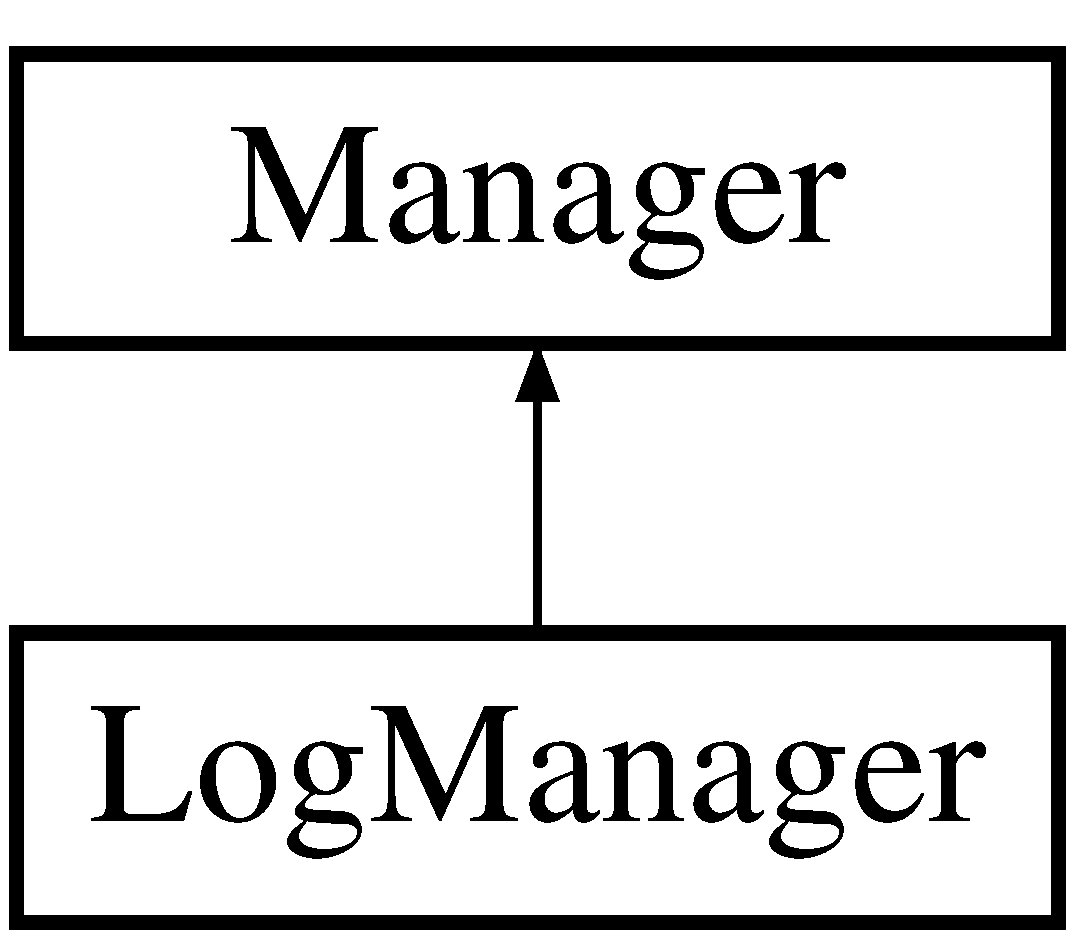
\includegraphics[height=2.000000cm]{class_log_manager}
\end{center}
\end{figure}
\subsection*{Public Member Functions}
\begin{DoxyCompactItemize}
\item 
int \hyperlink{class_log_manager_a61c2443f3923240ba6e7b74f89c4a50f}{start\+Up} ()
\item 
void \hyperlink{class_log_manager_a60520b802277e79880e78444d92dae93}{shut\+Down} ()
\item 
int \hyperlink{class_log_manager_a06b055d8fe1aef0f8b8cba3053f2d1ec}{write\+Log} (const char $\ast$fmt,...) const 
\item 
int \hyperlink{class_log_manager_a400f99a653cb542aa5e593cba35dd206}{write\+Log} (int log\+Level, const char $\ast$fmt,...) const 
\item 
void \hyperlink{class_log_manager_a94de253f71c67724e0b6de232129337a}{set\+Log\+Level} (int new\+Log\+Level)
\item 
int \hyperlink{class_log_manager_ae4bef18289c9990a2a0b9f58bc4c5470}{get\+Log\+Level} () const 
\item 
void \hyperlink{class_log_manager_abc6b0c8d7dd9fcb744540f9d18701563}{set\+Flush} (bool flush=true)
\end{DoxyCompactItemize}
\subsection*{Static Public Member Functions}
\begin{DoxyCompactItemize}
\item 
static \hyperlink{class_log_manager}{Log\+Manager} \& \hyperlink{class_log_manager_acd81e87b2d62ce40fceefcc55c4310ae}{get\+Instance} ()
\end{DoxyCompactItemize}


\subsection{Detailed Description}
\hyperlink{class_manager}{Manager} for writing info out to the log file 

\subsection{Member Function Documentation}
\hypertarget{class_log_manager_acd81e87b2d62ce40fceefcc55c4310ae}{\index{Log\+Manager@{Log\+Manager}!get\+Instance@{get\+Instance}}
\index{get\+Instance@{get\+Instance}!Log\+Manager@{Log\+Manager}}
\subsubsection[{get\+Instance}]{\setlength{\rightskip}{0pt plus 5cm}{\bf Log\+Manager} \& Log\+Manager\+::get\+Instance (
\begin{DoxyParamCaption}
{}
\end{DoxyParamCaption}
)\hspace{0.3cm}{\ttfamily [static]}}}\label{class_log_manager_acd81e87b2d62ce40fceefcc55c4310ae}
Gets the singleton instance of this object \begin{DoxyReturn}{Returns}
A reference to the log manager 
\end{DoxyReturn}
\hypertarget{class_log_manager_ae4bef18289c9990a2a0b9f58bc4c5470}{\index{Log\+Manager@{Log\+Manager}!get\+Log\+Level@{get\+Log\+Level}}
\index{get\+Log\+Level@{get\+Log\+Level}!Log\+Manager@{Log\+Manager}}
\subsubsection[{get\+Log\+Level}]{\setlength{\rightskip}{0pt plus 5cm}int Log\+Manager\+::get\+Log\+Level (
\begin{DoxyParamCaption}
{}
\end{DoxyParamCaption}
) const}}\label{class_log_manager_ae4bef18289c9990a2a0b9f58bc4c5470}
Gets the current log level of our logger \begin{DoxyReturn}{Returns}
The current log level 
\end{DoxyReturn}
\hypertarget{class_log_manager_abc6b0c8d7dd9fcb744540f9d18701563}{\index{Log\+Manager@{Log\+Manager}!set\+Flush@{set\+Flush}}
\index{set\+Flush@{set\+Flush}!Log\+Manager@{Log\+Manager}}
\subsubsection[{set\+Flush}]{\setlength{\rightskip}{0pt plus 5cm}void Log\+Manager\+::set\+Flush (
\begin{DoxyParamCaption}
\item[{bool}]{flush = {\ttfamily true}}
\end{DoxyParamCaption}
)}}\label{class_log_manager_abc6b0c8d7dd9fcb744540f9d18701563}
Sets if this logger should flush to file after each write 
\begin{DoxyParams}{Parameters}
{\em flush} & Indicates if we should flush, by default this is true \\
\hline
\end{DoxyParams}
\hypertarget{class_log_manager_a94de253f71c67724e0b6de232129337a}{\index{Log\+Manager@{Log\+Manager}!set\+Log\+Level@{set\+Log\+Level}}
\index{set\+Log\+Level@{set\+Log\+Level}!Log\+Manager@{Log\+Manager}}
\subsubsection[{set\+Log\+Level}]{\setlength{\rightskip}{0pt plus 5cm}void Log\+Manager\+::set\+Log\+Level (
\begin{DoxyParamCaption}
\item[{int}]{new\+Log\+Level}
\end{DoxyParamCaption}
)}}\label{class_log_manager_a94de253f71c67724e0b6de232129337a}
Sets the log level for our logger 
\begin{DoxyParams}{Parameters}
{\em new\+Log\+Level} & The new log level to use \\
\hline
\end{DoxyParams}
\hypertarget{class_log_manager_a60520b802277e79880e78444d92dae93}{\index{Log\+Manager@{Log\+Manager}!shut\+Down@{shut\+Down}}
\index{shut\+Down@{shut\+Down}!Log\+Manager@{Log\+Manager}}
\subsubsection[{shut\+Down}]{\setlength{\rightskip}{0pt plus 5cm}void Log\+Manager\+::shut\+Down (
\begin{DoxyParamCaption}
{}
\end{DoxyParamCaption}
)\hspace{0.3cm}{\ttfamily [virtual]}}}\label{class_log_manager_a60520b802277e79880e78444d92dae93}
Called to shutdown the log manager 

Reimplemented from \hyperlink{class_manager_a09f0aaf6012be52b75a12fac25370f61}{Manager}.

\hypertarget{class_log_manager_a61c2443f3923240ba6e7b74f89c4a50f}{\index{Log\+Manager@{Log\+Manager}!start\+Up@{start\+Up}}
\index{start\+Up@{start\+Up}!Log\+Manager@{Log\+Manager}}
\subsubsection[{start\+Up}]{\setlength{\rightskip}{0pt plus 5cm}int Log\+Manager\+::start\+Up (
\begin{DoxyParamCaption}
{}
\end{DoxyParamCaption}
)\hspace{0.3cm}{\ttfamily [virtual]}}}\label{class_log_manager_a61c2443f3923240ba6e7b74f89c4a50f}
Called when the log manager is started \begin{DoxyReturn}{Returns}
0 on success, a negative number when there is an error 
\end{DoxyReturn}


Reimplemented from \hyperlink{class_manager_a2a0f0d6810a5a051afd707d83ff1ff36}{Manager}.

\hypertarget{class_log_manager_a06b055d8fe1aef0f8b8cba3053f2d1ec}{\index{Log\+Manager@{Log\+Manager}!write\+Log@{write\+Log}}
\index{write\+Log@{write\+Log}!Log\+Manager@{Log\+Manager}}
\subsubsection[{write\+Log}]{\setlength{\rightskip}{0pt plus 5cm}int Log\+Manager\+::write\+Log (
\begin{DoxyParamCaption}
\item[{const char $\ast$}]{fmt, }
\item[{}]{...}
\end{DoxyParamCaption}
) const}}\label{class_log_manager_a06b055d8fe1aef0f8b8cba3053f2d1ec}
Writes a formatted string to the log 
\begin{DoxyParams}{Parameters}
{\em fmt} & The string format to use \\
\hline
\end{DoxyParams}
\begin{DoxyReturn}{Returns}
the number of bytes written to the log 
\end{DoxyReturn}
\hypertarget{class_log_manager_a400f99a653cb542aa5e593cba35dd206}{\index{Log\+Manager@{Log\+Manager}!write\+Log@{write\+Log}}
\index{write\+Log@{write\+Log}!Log\+Manager@{Log\+Manager}}
\subsubsection[{write\+Log}]{\setlength{\rightskip}{0pt plus 5cm}int Log\+Manager\+::write\+Log (
\begin{DoxyParamCaption}
\item[{int}]{log\+Level, }
\item[{const char $\ast$}]{fmt, }
\item[{}]{...}
\end{DoxyParamCaption}
) const}}\label{class_log_manager_a400f99a653cb542aa5e593cba35dd206}
Writes a formatted string to the log if we are at or above the current log level 
\begin{DoxyParams}{Parameters}
{\em log\+Level} & The log level of this message \\
\hline
{\em fmt} & The string format to use \\
\hline
\end{DoxyParams}
\begin{DoxyReturn}{Returns}
The number of bytes written to the log 
\end{DoxyReturn}


The documentation for this class was generated from the following files\+:\begin{DoxyCompactItemize}
\item 
F\+:/\+Users/\+Benny/git/\+I\+M\+G\+D3000/\+I\+M\+G\+D3000\+Proj3/include/Log\+Manager.\+h\item 
F\+:/\+Users/\+Benny/git/\+I\+M\+G\+D3000/\+I\+M\+G\+D3000\+Proj3/lib/src/\+Core/Log\+Manager.\+cpp\end{DoxyCompactItemize}

\hypertarget{class_manager}{\section{Manager Class Reference}
\label{class_manager}\index{Manager@{Manager}}
}


{\ttfamily \#include $<$Manager.\+h$>$}

Inheritance diagram for Manager\+:\begin{figure}[H]
\begin{center}
\leavevmode
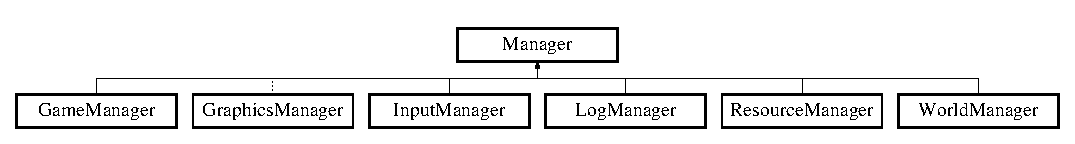
\includegraphics[height=1.493333cm]{class_manager}
\end{center}
\end{figure}
\subsection*{Public Member Functions}
\begin{DoxyCompactItemize}
\item 
virtual int \hyperlink{class_manager_a2a0f0d6810a5a051afd707d83ff1ff36}{start\+Up} ()
\item 
virtual void \hyperlink{class_manager_a09f0aaf6012be52b75a12fac25370f61}{shut\+Down} ()
\item 
bool \hyperlink{class_manager_aa5b4c6cc66d0bb5e803d9fab953a1b39}{has\+Started} () const 
\item 
virtual int \hyperlink{class_manager_abfdbe16dc74a246b70a183351e100989}{on\+Event} (\hyperlink{class_event}{Event} $\ast$e) const 
\end{DoxyCompactItemize}


\subsection{Detailed Description}
Base class for all managers in the engine 

\subsection{Member Function Documentation}
\hypertarget{class_manager_aa5b4c6cc66d0bb5e803d9fab953a1b39}{\index{Manager@{Manager}!has\+Started@{has\+Started}}
\index{has\+Started@{has\+Started}!Manager@{Manager}}
\subsubsection[{has\+Started}]{\setlength{\rightskip}{0pt plus 5cm}bool Manager\+::has\+Started (
\begin{DoxyParamCaption}
{}
\end{DoxyParamCaption}
) const}}\label{class_manager_aa5b4c6cc66d0bb5e803d9fab953a1b39}
Indicates whether the manager has been started or not \begin{DoxyReturn}{Returns}
True if this manager has been started, false otherwise 
\end{DoxyReturn}
\hypertarget{class_manager_abfdbe16dc74a246b70a183351e100989}{\index{Manager@{Manager}!on\+Event@{on\+Event}}
\index{on\+Event@{on\+Event}!Manager@{Manager}}
\subsubsection[{on\+Event}]{\setlength{\rightskip}{0pt plus 5cm}int Manager\+::on\+Event (
\begin{DoxyParamCaption}
\item[{{\bf Event} $\ast$}]{e}
\end{DoxyParamCaption}
) const\hspace{0.3cm}{\ttfamily [virtual]}}}\label{class_manager_abfdbe16dc74a246b70a183351e100989}
Used to pass events to a manager 
\begin{DoxyParams}{Parameters}
{\em e} & The event to pass \\
\hline
\end{DoxyParams}
\begin{DoxyReturn}{Returns}
1 if the event was able to be passed, 0 otherwise 
\end{DoxyReturn}


Reimplemented in \hyperlink{class_world_manager_a72462c64fa931378504f18a2966c303d}{World\+Manager}.

\hypertarget{class_manager_a09f0aaf6012be52b75a12fac25370f61}{\index{Manager@{Manager}!shut\+Down@{shut\+Down}}
\index{shut\+Down@{shut\+Down}!Manager@{Manager}}
\subsubsection[{shut\+Down}]{\setlength{\rightskip}{0pt plus 5cm}void Manager\+::shut\+Down (
\begin{DoxyParamCaption}
{}
\end{DoxyParamCaption}
)\hspace{0.3cm}{\ttfamily [virtual]}}}\label{class_manager_a09f0aaf6012be52b75a12fac25370f61}
Shuts down the manager 

Reimplemented in \hyperlink{class_world_manager_a94c6c0dae961c535b6f2f543e029d6b6}{World\+Manager}, \hyperlink{class_graphics_manager_a5d850ef5d3a6792eb270fa22b784b3e6}{Graphics\+Manager}, \hyperlink{class_game_manager_a6cbd6266472fb9c0b08a4c2f7f8813af}{Game\+Manager}, \hyperlink{class_log_manager_a60520b802277e79880e78444d92dae93}{Log\+Manager}, \hyperlink{class_input_manager_ad9ae425dbb849fda4616484e7156600e}{Input\+Manager}, and \hyperlink{class_resource_manager_a6db779a2721e927cffb9f0c7ab31495c}{Resource\+Manager}.

\hypertarget{class_manager_a2a0f0d6810a5a051afd707d83ff1ff36}{\index{Manager@{Manager}!start\+Up@{start\+Up}}
\index{start\+Up@{start\+Up}!Manager@{Manager}}
\subsubsection[{start\+Up}]{\setlength{\rightskip}{0pt plus 5cm}int Manager\+::start\+Up (
\begin{DoxyParamCaption}
{}
\end{DoxyParamCaption}
)\hspace{0.3cm}{\ttfamily [virtual]}}}\label{class_manager_a2a0f0d6810a5a051afd707d83ff1ff36}
Called to start the manager \begin{DoxyReturn}{Returns}
0 if ok, a number $<$ 0 if an error occurred 
\end{DoxyReturn}


Reimplemented in \hyperlink{class_world_manager_a7ad9c0bf4968b08b82d7d7daa159943a}{World\+Manager}, \hyperlink{class_graphics_manager_ac1961e1b4985a41a6eb233736d5d3191}{Graphics\+Manager}, \hyperlink{class_game_manager_a6626dd9f245039379b3416e2a28bb71c}{Game\+Manager}, \hyperlink{class_log_manager_a61c2443f3923240ba6e7b74f89c4a50f}{Log\+Manager}, \hyperlink{class_input_manager_a210997e45748bae7d0901ac3ede788c6}{Input\+Manager}, and \hyperlink{class_resource_manager_a53bf358b029e050a285725bc70a8550a}{Resource\+Manager}.



The documentation for this class was generated from the following files\+:\begin{DoxyCompactItemize}
\item 
F\+:/\+Users/\+Benny/git/\+I\+M\+G\+D3000/\+I\+M\+G\+D3000\+Proj3/include/Manager.\+h\item 
F\+:/\+Users/\+Benny/git/\+I\+M\+G\+D3000/\+I\+M\+G\+D3000\+Proj3/lib/src/\+Core/Manager.\+cpp\end{DoxyCompactItemize}

\hypertarget{class_object}{\section{Object Class Reference}
\label{class_object}\index{Object@{Object}}
}


{\ttfamily \#include $<$Object.\+h$>$}

Inheritance diagram for Object\+:\begin{figure}[H]
\begin{center}
\leavevmode
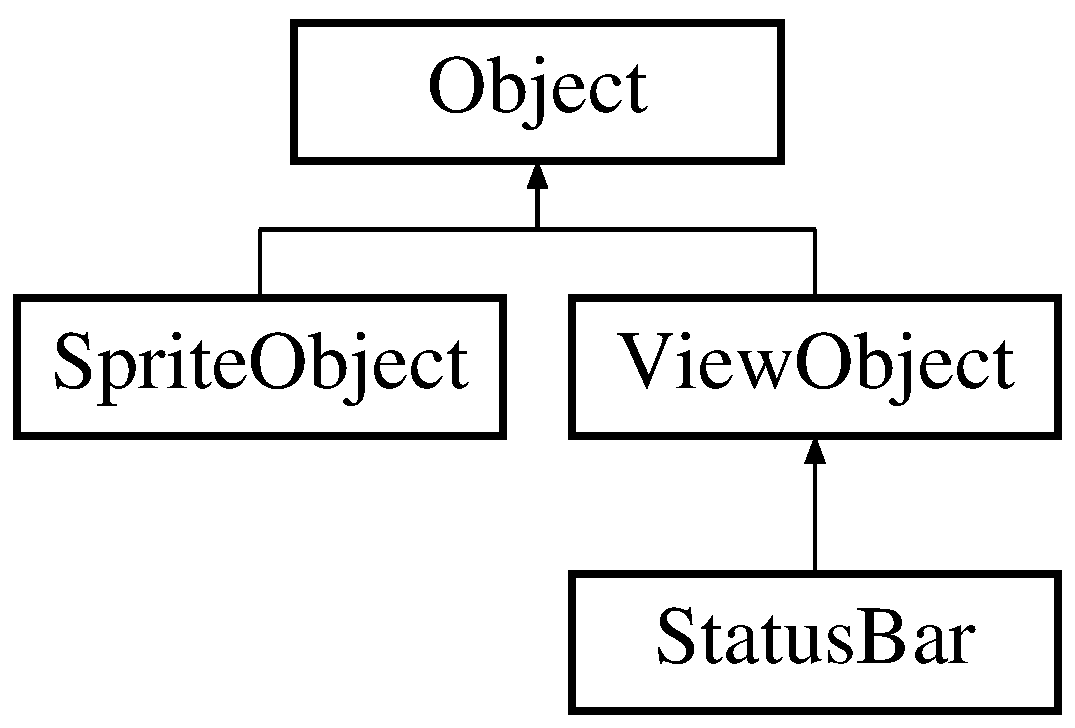
\includegraphics[height=3.000000cm]{class_object}
\end{center}
\end{figure}
\subsection*{Public Member Functions}
\begin{DoxyCompactItemize}
\item 
\hyperlink{class_object_a40860402e64d8008fb42329df7097cdb}{Object} ()
\item 
virtual \hyperlink{class_object_ae8f5483f459e46687bd01e6f9977afd3}{$\sim$\+Object} ()
\item 
int \hyperlink{class_object_a5d973a1f45b51420a8bfb324ef2c25f7}{set\+I\+D} (unsigned int new\+I\+D)
\item 
unsigned int \hyperlink{class_object_ac62e10ee5bcc2b7855fa0bae401b2ca7}{get\+I\+D} () const 
\item 
string \hyperlink{class_object_af18945ab6296dc8f0ea0d9517446020a}{get\+Type} () const 
\item 
void \hyperlink{class_object_a4ea1a63afb9ac3fdb61dbcd23c86ce33}{set\+Type} (string type)
\item 
bool \hyperlink{class_object_aa8e7d1dab28e847c2c7308dcfdcb3530}{set\+Solidness} (Solidness solidness)
\item 
Solidness \hyperlink{class_object_a15c18dc963ca3e6b79ec5cbb7c187600}{get\+Solidness} () const 
\item 
bool \hyperlink{class_object_a0d2e685ed20b49ec1b7feeba4c0f1cc9}{is\+Collidable} ()
\item 
void \hyperlink{class_object_a996264e469eaa68ff31884fda5ba60e1}{set\+Altitude} (unsigned int value)
\item 
unsigned int \hyperlink{class_object_aa683addeedbb34a8932bbc6c2a240fab}{get\+Altitude} () const 
\item 
void \hyperlink{class_object_aaa4e4c388b9bdf9a9f341351d297c5ed}{set\+Position} (\hyperlink{class_i_vector}{I\+Vector} new\+Position)
\item 
\hyperlink{class_i_vector}{I\+Vector} \hyperlink{class_object_a548a4a71f26f3c0182dcad383a1877b9}{get\+Position} () const 
\item 
void \hyperlink{class_object_a3b8758e206b78d43da2c0e96389d9dc0}{set\+Velocity} (\hyperlink{class_f_vector}{F\+Vector} velocity)
\item 
void \hyperlink{class_object_a16ad5e2c57e31cd94dac983d26a7460f}{set\+Velocity\+X} (float x)
\item 
void \hyperlink{class_object_a0596584fa3ce951c36fcdc423911c84a}{set\+Velocity\+Y} (float y)
\item 
\hyperlink{class_f_vector}{F\+Vector} \hyperlink{class_object_a4f1958fae32120d02efcecd7b1beab0a}{get\+Velocity} () const 
\item 
float \hyperlink{class_object_a38db2c22257704f142a381489a14fab7}{get\+Velocity\+X} () const 
\item 
float \hyperlink{class_object_abaa3cb97d49316883310e039de172dd4}{get\+Velocity\+Y} () const 
\item 
\hyperlink{class_i_vector}{I\+Vector} \hyperlink{class_object_a3589d53e0f2594f92b946b1b40a07c75}{get\+Velocity\+Step} ()
\item 
\hyperlink{class_box}{Box} \hyperlink{class_object_a75472ab21010cf9c8da2046076ec09e1}{get\+Bounds} () const 
\item 
void \hyperlink{class_object_a2ee8e04108059dc5ca44ef6bfdc8543f}{set\+Bounds} (\hyperlink{class_box}{Box} bounds)
\item 
\hyperlink{class_box}{Box} \hyperlink{class_object_abc47b6c91a4ea3605c00039c5c8ba0f3}{get\+World\+Bounds} () const 
\item 
\hyperlink{class_box}{Box} \hyperlink{class_object_a478c8650ee8250fc9d44c0a6e8b6c5f2}{get\+World\+Bounds} (const \hyperlink{class_i_vector}{I\+Vector} \&position) const 
\item 
\hyperlink{class_sprite}{Sprite} $\ast$ \hyperlink{class_object_aae255594aef34a3db3bd15b5af41a5af}{get\+Sprite} () const 
\item 
void \hyperlink{class_object_adabc85f4c580093594250b677b8573d7}{set\+Sprite} (\hyperlink{class_sprite}{Sprite} $\ast$sprite, bool set\+Box=true)
\item 
bool \hyperlink{class_object_a517454b636773a14b7710b78734056f3}{is\+Centered} () const 
\item 
void \hyperlink{class_object_a8eac55a24936bb18524c96fe00189404}{set\+Centered} (bool centered)
\item 
void \hyperlink{class_object_add0a363fc8351f966979f61c75232bd9}{set\+Frame\+Index} (int frame)
\item 
int \hyperlink{class_object_a85ef29d394641a1f96cab82217245d51}{get\+Frame\+Index} () const 
\item 
void \hyperlink{class_object_ab753d38950b3e3ea3a0d1c53c4912c38}{set\+Slowdown} (int slowdown)
\item 
int \hyperlink{class_object_aeec8faca38e258b6ec6b5298956c15b2}{get\+Slowdown} () const 
\item 
void \hyperlink{class_object_a937aa61549bbcea2c02f43ae24cd73ef}{set\+Color} (int color)
\item 
int \hyperlink{class_object_ae5e6499a684d0e46c2609b219650e598}{get\+Color} () const 
\item 
virtual int \hyperlink{class_object_aef5d6ac71c5184a72e7101584d377998}{event\+Handler} (\hyperlink{class_event}{Event} $\ast$e)
\item 
virtual void \hyperlink{class_object_a821f5b25b450fa1acdb3f9c0b5962592}{draw} ()
\end{DoxyCompactItemize}


\subsection{Detailed Description}
The base class for all objects 

\subsection{Constructor \& Destructor Documentation}
\hypertarget{class_object_a40860402e64d8008fb42329df7097cdb}{\index{Object@{Object}!Object@{Object}}
\index{Object@{Object}!Object@{Object}}
\subsubsection[{Object}]{\setlength{\rightskip}{0pt plus 5cm}Object\+::\+Object (
\begin{DoxyParamCaption}
{}
\end{DoxyParamCaption}
)}}\label{class_object_a40860402e64d8008fb42329df7097cdb}
Creates a new object in the world \hypertarget{class_object_ae8f5483f459e46687bd01e6f9977afd3}{\index{Object@{Object}!````~Object@{$\sim$\+Object}}
\index{````~Object@{$\sim$\+Object}!Object@{Object}}
\subsubsection[{$\sim$\+Object}]{\setlength{\rightskip}{0pt plus 5cm}Object\+::$\sim$\+Object (
\begin{DoxyParamCaption}
{}
\end{DoxyParamCaption}
)\hspace{0.3cm}{\ttfamily [virtual]}}}\label{class_object_ae8f5483f459e46687bd01e6f9977afd3}
D\+O N\+O\+T C\+A\+L\+L T\+H\+R\+O\+U\+G\+H D\+E\+L\+E\+T\+E, C\+A\+L\+L T\+H\+R\+O\+U\+G\+H M\+A\+R\+K F\+O\+R D\+E\+L\+E\+T\+E 

\subsection{Member Function Documentation}
\hypertarget{class_object_a821f5b25b450fa1acdb3f9c0b5962592}{\index{Object@{Object}!draw@{draw}}
\index{draw@{draw}!Object@{Object}}
\subsubsection[{draw}]{\setlength{\rightskip}{0pt plus 5cm}void Object\+::draw (
\begin{DoxyParamCaption}
{}
\end{DoxyParamCaption}
)\hspace{0.3cm}{\ttfamily [virtual]}}}\label{class_object_a821f5b25b450fa1acdb3f9c0b5962592}
Called once per frame to draw the object 

Reimplemented in \hyperlink{class_view_object_aae76e90e25d65e34d80e468b41af95da}{View\+Object}, \hyperlink{class_tester_object_a89ca89d9a75a1aa07f7de7fdd3a3eab7}{Tester\+Object}, \hyperlink{class_test_object_solid_a4a4bbaa86d29b0294134b89a6e4d77be}{Test\+Object\+Solid}, and \hyperlink{class_test_object_soft_ab08f5c7bf248ff21e4fcffe3b4a053e9}{Test\+Object\+Soft}.

\hypertarget{class_object_aef5d6ac71c5184a72e7101584d377998}{\index{Object@{Object}!event\+Handler@{event\+Handler}}
\index{event\+Handler@{event\+Handler}!Object@{Object}}
\subsubsection[{event\+Handler}]{\setlength{\rightskip}{0pt plus 5cm}int Object\+::event\+Handler (
\begin{DoxyParamCaption}
\item[{{\bf Event} $\ast$}]{e}
\end{DoxyParamCaption}
)\hspace{0.3cm}{\ttfamily [virtual]}}}\label{class_object_aef5d6ac71c5184a72e7101584d377998}
Handles events given to this object 
\begin{DoxyParams}{Parameters}
{\em e} & A pointer to the event data \\
\hline
\end{DoxyParams}
\begin{DoxyReturn}{Returns}
a non-\/zero number if this object does consume the event, otherwise 0 
\end{DoxyReturn}


Reimplemented in \hyperlink{class_view_object_aae06f1481afddf829a97b045a0c60bb7}{View\+Object}, \hyperlink{class_tester_object_aa9991d352e5745062f4e040c3f812b4d}{Tester\+Object}, \hyperlink{class_test_object_solid_a74649b5b4fd341268f2938e9b2d9ebf3}{Test\+Object\+Solid}, and \hyperlink{class_test_object_soft_a3eb882515691114d9eb09455468cf4fd}{Test\+Object\+Soft}.

\hypertarget{class_object_aa683addeedbb34a8932bbc6c2a240fab}{\index{Object@{Object}!get\+Altitude@{get\+Altitude}}
\index{get\+Altitude@{get\+Altitude}!Object@{Object}}
\subsubsection[{get\+Altitude}]{\setlength{\rightskip}{0pt plus 5cm}unsigned int Object\+::get\+Altitude (
\begin{DoxyParamCaption}
{}
\end{DoxyParamCaption}
) const}}\label{class_object_aa683addeedbb34a8932bbc6c2a240fab}
Get the render order of this object \begin{DoxyReturn}{Returns}
The altitude as an unsigned int 
\end{DoxyReturn}
\hypertarget{class_object_a75472ab21010cf9c8da2046076ec09e1}{\index{Object@{Object}!get\+Bounds@{get\+Bounds}}
\index{get\+Bounds@{get\+Bounds}!Object@{Object}}
\subsubsection[{get\+Bounds}]{\setlength{\rightskip}{0pt plus 5cm}{\bf Box} Object\+::get\+Bounds (
\begin{DoxyParamCaption}
{}
\end{DoxyParamCaption}
) const}}\label{class_object_a75472ab21010cf9c8da2046076ec09e1}
Get the bounding box for this object \begin{DoxyReturn}{Returns}
The objects bounding box 
\end{DoxyReturn}
\hypertarget{class_object_ae5e6499a684d0e46c2609b219650e598}{\index{Object@{Object}!get\+Color@{get\+Color}}
\index{get\+Color@{get\+Color}!Object@{Object}}
\subsubsection[{get\+Color}]{\setlength{\rightskip}{0pt plus 5cm}int Object\+::get\+Color (
\begin{DoxyParamCaption}
{}
\end{DoxyParamCaption}
) const}}\label{class_object_ae5e6499a684d0e46c2609b219650e598}
Gets the color to draw the object with \begin{DoxyReturn}{Returns}
The color to draw the object with 
\end{DoxyReturn}
\hypertarget{class_object_a85ef29d394641a1f96cab82217245d51}{\index{Object@{Object}!get\+Frame\+Index@{get\+Frame\+Index}}
\index{get\+Frame\+Index@{get\+Frame\+Index}!Object@{Object}}
\subsubsection[{get\+Frame\+Index}]{\setlength{\rightskip}{0pt plus 5cm}int Object\+::get\+Frame\+Index (
\begin{DoxyParamCaption}
{}
\end{DoxyParamCaption}
) const}}\label{class_object_a85ef29d394641a1f96cab82217245d51}
Gets the index of the current frame of the sprite \begin{DoxyReturn}{Returns}
The index of the current frame 
\end{DoxyReturn}
\hypertarget{class_object_ac62e10ee5bcc2b7855fa0bae401b2ca7}{\index{Object@{Object}!get\+I\+D@{get\+I\+D}}
\index{get\+I\+D@{get\+I\+D}!Object@{Object}}
\subsubsection[{get\+I\+D}]{\setlength{\rightskip}{0pt plus 5cm}unsigned int Object\+::get\+I\+D (
\begin{DoxyParamCaption}
{}
\end{DoxyParamCaption}
) const}}\label{class_object_ac62e10ee5bcc2b7855fa0bae401b2ca7}
Gets the I\+D of this object \begin{DoxyReturn}{Returns}
The object I\+D 
\end{DoxyReturn}
\hypertarget{class_object_a548a4a71f26f3c0182dcad383a1877b9}{\index{Object@{Object}!get\+Position@{get\+Position}}
\index{get\+Position@{get\+Position}!Object@{Object}}
\subsubsection[{get\+Position}]{\setlength{\rightskip}{0pt plus 5cm}{\bf I\+Vector} Object\+::get\+Position (
\begin{DoxyParamCaption}
{}
\end{DoxyParamCaption}
) const}}\label{class_object_a548a4a71f26f3c0182dcad383a1877b9}
Gets the current position of this object \begin{DoxyReturn}{Returns}
The position of this object 
\end{DoxyReturn}
\hypertarget{class_object_aeec8faca38e258b6ec6b5298956c15b2}{\index{Object@{Object}!get\+Slowdown@{get\+Slowdown}}
\index{get\+Slowdown@{get\+Slowdown}!Object@{Object}}
\subsubsection[{get\+Slowdown}]{\setlength{\rightskip}{0pt plus 5cm}int Object\+::get\+Slowdown (
\begin{DoxyParamCaption}
{}
\end{DoxyParamCaption}
) const}}\label{class_object_aeec8faca38e258b6ec6b5298956c15b2}
Gets the slowdown for the animation \begin{DoxyReturn}{Returns}
The number of frames to wait before drawing the next frame 
\end{DoxyReturn}
\hypertarget{class_object_a15c18dc963ca3e6b79ec5cbb7c187600}{\index{Object@{Object}!get\+Solidness@{get\+Solidness}}
\index{get\+Solidness@{get\+Solidness}!Object@{Object}}
\subsubsection[{get\+Solidness}]{\setlength{\rightskip}{0pt plus 5cm}Solidness Object\+::get\+Solidness (
\begin{DoxyParamCaption}
{}
\end{DoxyParamCaption}
) const}}\label{class_object_a15c18dc963ca3e6b79ec5cbb7c187600}
Gets the collision model to use with this object \begin{DoxyReturn}{Returns}
The collision model that this object is using 
\end{DoxyReturn}
\hypertarget{class_object_aae255594aef34a3db3bd15b5af41a5af}{\index{Object@{Object}!get\+Sprite@{get\+Sprite}}
\index{get\+Sprite@{get\+Sprite}!Object@{Object}}
\subsubsection[{get\+Sprite}]{\setlength{\rightskip}{0pt plus 5cm}{\bf Sprite} $\ast$ Object\+::get\+Sprite (
\begin{DoxyParamCaption}
{}
\end{DoxyParamCaption}
) const}}\label{class_object_aae255594aef34a3db3bd15b5af41a5af}
Gets the sprite that this object uses \begin{DoxyReturn}{Returns}
The sprite this object uses or N\+U\+L\+L if there is none 
\end{DoxyReturn}
\hypertarget{class_object_af18945ab6296dc8f0ea0d9517446020a}{\index{Object@{Object}!get\+Type@{get\+Type}}
\index{get\+Type@{get\+Type}!Object@{Object}}
\subsubsection[{get\+Type}]{\setlength{\rightskip}{0pt plus 5cm}string Object\+::get\+Type (
\begin{DoxyParamCaption}
{}
\end{DoxyParamCaption}
) const}}\label{class_object_af18945ab6296dc8f0ea0d9517446020a}
Gets the type name of this object \begin{DoxyReturn}{Returns}
The type name of this object 
\end{DoxyReturn}
\hypertarget{class_object_a4f1958fae32120d02efcecd7b1beab0a}{\index{Object@{Object}!get\+Velocity@{get\+Velocity}}
\index{get\+Velocity@{get\+Velocity}!Object@{Object}}
\subsubsection[{get\+Velocity}]{\setlength{\rightskip}{0pt plus 5cm}{\bf F\+Vector} Object\+::get\+Velocity (
\begin{DoxyParamCaption}
{}
\end{DoxyParamCaption}
) const}}\label{class_object_a4f1958fae32120d02efcecd7b1beab0a}
Gets the velocity of the object \begin{DoxyReturn}{Returns}
An \hyperlink{class_f_vector}{F\+Vector} that represents the x and y velocity 
\end{DoxyReturn}
\hypertarget{class_object_a3589d53e0f2594f92b946b1b40a07c75}{\index{Object@{Object}!get\+Velocity\+Step@{get\+Velocity\+Step}}
\index{get\+Velocity\+Step@{get\+Velocity\+Step}!Object@{Object}}
\subsubsection[{get\+Velocity\+Step}]{\setlength{\rightskip}{0pt plus 5cm}{\bf I\+Vector} Object\+::get\+Velocity\+Step (
\begin{DoxyParamCaption}
{}
\end{DoxyParamCaption}
)}}\label{class_object_a3589d53e0f2594f92b946b1b40a07c75}
Steps the object one frame forward \begin{DoxyReturn}{Returns}
The amount moved this frame 
\end{DoxyReturn}
\hypertarget{class_object_a38db2c22257704f142a381489a14fab7}{\index{Object@{Object}!get\+Velocity\+X@{get\+Velocity\+X}}
\index{get\+Velocity\+X@{get\+Velocity\+X}!Object@{Object}}
\subsubsection[{get\+Velocity\+X}]{\setlength{\rightskip}{0pt plus 5cm}float Object\+::get\+Velocity\+X (
\begin{DoxyParamCaption}
{}
\end{DoxyParamCaption}
) const}}\label{class_object_a38db2c22257704f142a381489a14fab7}
Gets the x velocity of the object \begin{DoxyReturn}{Returns}
A floating point number that is the x velocity of the object in units/step 
\end{DoxyReturn}
\hypertarget{class_object_abaa3cb97d49316883310e039de172dd4}{\index{Object@{Object}!get\+Velocity\+Y@{get\+Velocity\+Y}}
\index{get\+Velocity\+Y@{get\+Velocity\+Y}!Object@{Object}}
\subsubsection[{get\+Velocity\+Y}]{\setlength{\rightskip}{0pt plus 5cm}float Object\+::get\+Velocity\+Y (
\begin{DoxyParamCaption}
{}
\end{DoxyParamCaption}
) const}}\label{class_object_abaa3cb97d49316883310e039de172dd4}
Gets the y velocity of the object \begin{DoxyReturn}{Returns}
A floating point number that is the y velocity of the object in units/step 
\end{DoxyReturn}
\hypertarget{class_object_abc47b6c91a4ea3605c00039c5c8ba0f3}{\index{Object@{Object}!get\+World\+Bounds@{get\+World\+Bounds}}
\index{get\+World\+Bounds@{get\+World\+Bounds}!Object@{Object}}
\subsubsection[{get\+World\+Bounds}]{\setlength{\rightskip}{0pt plus 5cm}{\bf Box} Object\+::get\+World\+Bounds (
\begin{DoxyParamCaption}
{}
\end{DoxyParamCaption}
) const}}\label{class_object_abc47b6c91a4ea3605c00039c5c8ba0f3}
Gets the objects bounds in world space \begin{DoxyReturn}{Returns}
The objects bounds in world space 
\end{DoxyReturn}
\hypertarget{class_object_a478c8650ee8250fc9d44c0a6e8b6c5f2}{\index{Object@{Object}!get\+World\+Bounds@{get\+World\+Bounds}}
\index{get\+World\+Bounds@{get\+World\+Bounds}!Object@{Object}}
\subsubsection[{get\+World\+Bounds}]{\setlength{\rightskip}{0pt plus 5cm}{\bf Box} Object\+::get\+World\+Bounds (
\begin{DoxyParamCaption}
\item[{const {\bf I\+Vector} \&}]{position}
\end{DoxyParamCaption}
) const}}\label{class_object_a478c8650ee8250fc9d44c0a6e8b6c5f2}
Gets an objects bounds in world space as though the object is at a different position 
\begin{DoxyParams}{Parameters}
{\em position} & The new position to say the object is at \\
\hline
\end{DoxyParams}
\begin{DoxyReturn}{Returns}
The objects bounds in world space relative to the position 
\end{DoxyReturn}
\hypertarget{class_object_a517454b636773a14b7710b78734056f3}{\index{Object@{Object}!is\+Centered@{is\+Centered}}
\index{is\+Centered@{is\+Centered}!Object@{Object}}
\subsubsection[{is\+Centered}]{\setlength{\rightskip}{0pt plus 5cm}bool Object\+::is\+Centered (
\begin{DoxyParamCaption}
{}
\end{DoxyParamCaption}
) const}}\label{class_object_a517454b636773a14b7710b78734056f3}
Checks to see if this object is centered on its position \begin{DoxyReturn}{Returns}
True if it is centered, false otherwise 
\end{DoxyReturn}
\hypertarget{class_object_a0d2e685ed20b49ec1b7feeba4c0f1cc9}{\index{Object@{Object}!is\+Collidable@{is\+Collidable}}
\index{is\+Collidable@{is\+Collidable}!Object@{Object}}
\subsubsection[{is\+Collidable}]{\setlength{\rightskip}{0pt plus 5cm}bool Object\+::is\+Collidable (
\begin{DoxyParamCaption}
{}
\end{DoxyParamCaption}
)}}\label{class_object_a0d2e685ed20b49ec1b7feeba4c0f1cc9}
Checks to see if the object will have a collision \begin{DoxyReturn}{Returns}
True if collision model is set to H\+A\+R\+D or S\+O\+F\+T, otherwise false 
\end{DoxyReturn}
\hypertarget{class_object_a996264e469eaa68ff31884fda5ba60e1}{\index{Object@{Object}!set\+Altitude@{set\+Altitude}}
\index{set\+Altitude@{set\+Altitude}!Object@{Object}}
\subsubsection[{set\+Altitude}]{\setlength{\rightskip}{0pt plus 5cm}void Object\+::set\+Altitude (
\begin{DoxyParamCaption}
\item[{unsigned int}]{value}
\end{DoxyParamCaption}
)}}\label{class_object_a996264e469eaa68ff31884fda5ba60e1}
Set the render order of this object 
\begin{DoxyParams}{Parameters}
{\em value} & The new value to set altitude to \\
\hline
\end{DoxyParams}
\hypertarget{class_object_a2ee8e04108059dc5ca44ef6bfdc8543f}{\index{Object@{Object}!set\+Bounds@{set\+Bounds}}
\index{set\+Bounds@{set\+Bounds}!Object@{Object}}
\subsubsection[{set\+Bounds}]{\setlength{\rightskip}{0pt plus 5cm}void Object\+::set\+Bounds (
\begin{DoxyParamCaption}
\item[{{\bf Box}}]{bounds}
\end{DoxyParamCaption}
)}}\label{class_object_a2ee8e04108059dc5ca44ef6bfdc8543f}
Sets the bounding box for this object 
\begin{DoxyParams}{Parameters}
{\em bounds} & The new bounding box \\
\hline
\end{DoxyParams}
\hypertarget{class_object_a8eac55a24936bb18524c96fe00189404}{\index{Object@{Object}!set\+Centered@{set\+Centered}}
\index{set\+Centered@{set\+Centered}!Object@{Object}}
\subsubsection[{set\+Centered}]{\setlength{\rightskip}{0pt plus 5cm}void Object\+::set\+Centered (
\begin{DoxyParamCaption}
\item[{bool}]{centered}
\end{DoxyParamCaption}
)}}\label{class_object_a8eac55a24936bb18524c96fe00189404}
Sets if this object should be centered on its world position or not 
\begin{DoxyParams}{Parameters}
{\em centered} & If true the object will be centered, if false the object will not \\
\hline
\end{DoxyParams}
\hypertarget{class_object_a937aa61549bbcea2c02f43ae24cd73ef}{\index{Object@{Object}!set\+Color@{set\+Color}}
\index{set\+Color@{set\+Color}!Object@{Object}}
\subsubsection[{set\+Color}]{\setlength{\rightskip}{0pt plus 5cm}void Object\+::set\+Color (
\begin{DoxyParamCaption}
\item[{int}]{color}
\end{DoxyParamCaption}
)}}\label{class_object_a937aa61549bbcea2c02f43ae24cd73ef}
Sets the color to draw the object with 
\begin{DoxyParams}{Parameters}
{\em color} & The color to draw the object with \\
\hline
\end{DoxyParams}
\hypertarget{class_object_add0a363fc8351f966979f61c75232bd9}{\index{Object@{Object}!set\+Frame\+Index@{set\+Frame\+Index}}
\index{set\+Frame\+Index@{set\+Frame\+Index}!Object@{Object}}
\subsubsection[{set\+Frame\+Index}]{\setlength{\rightskip}{0pt plus 5cm}void Object\+::set\+Frame\+Index (
\begin{DoxyParamCaption}
\item[{int}]{frame}
\end{DoxyParamCaption}
)}}\label{class_object_add0a363fc8351f966979f61c75232bd9}
Sets the current frame that the object should render 
\begin{DoxyParams}{Parameters}
{\em frame} & The index of the frame in the sprite, if this number is out of bounds it will be wrapped around to fit \\
\hline
\end{DoxyParams}
\hypertarget{class_object_a5d973a1f45b51420a8bfb324ef2c25f7}{\index{Object@{Object}!set\+I\+D@{set\+I\+D}}
\index{set\+I\+D@{set\+I\+D}!Object@{Object}}
\subsubsection[{set\+I\+D}]{\setlength{\rightskip}{0pt plus 5cm}int Object\+::set\+I\+D (
\begin{DoxyParamCaption}
\item[{unsigned int}]{new\+I\+D}
\end{DoxyParamCaption}
)}}\label{class_object_a5d973a1f45b51420a8bfb324ef2c25f7}
Changes this objects id to the new I\+D 
\begin{DoxyParams}{Parameters}
{\em new\+I\+D} & The new id to change this objects id to \\
\hline
\end{DoxyParams}
\begin{DoxyReturn}{Returns}
returns the new id that was assigned, or 0 on fail 
\end{DoxyReturn}
\begin{DoxyRemark}{Remarks}
When the id is failed to be set we will not go to a 0 id but just keep the old id 
\end{DoxyRemark}
\hypertarget{class_object_aaa4e4c388b9bdf9a9f341351d297c5ed}{\index{Object@{Object}!set\+Position@{set\+Position}}
\index{set\+Position@{set\+Position}!Object@{Object}}
\subsubsection[{set\+Position}]{\setlength{\rightskip}{0pt plus 5cm}void Object\+::set\+Position (
\begin{DoxyParamCaption}
\item[{{\bf I\+Vector}}]{new\+Position}
\end{DoxyParamCaption}
)}}\label{class_object_aaa4e4c388b9bdf9a9f341351d297c5ed}
Changes the objects position 
\begin{DoxyParams}{Parameters}
{\em new\+Position} & The new position this object should be at \\
\hline
\end{DoxyParams}
\hypertarget{class_object_ab753d38950b3e3ea3a0d1c53c4912c38}{\index{Object@{Object}!set\+Slowdown@{set\+Slowdown}}
\index{set\+Slowdown@{set\+Slowdown}!Object@{Object}}
\subsubsection[{set\+Slowdown}]{\setlength{\rightskip}{0pt plus 5cm}void Object\+::set\+Slowdown (
\begin{DoxyParamCaption}
\item[{int}]{slowdown}
\end{DoxyParamCaption}
)}}\label{class_object_ab753d38950b3e3ea3a0d1c53c4912c38}
Sets the slowdown on the animation 
\begin{DoxyParams}{Parameters}
{\em slowdown} & The number of frames to wait before drawing the next frame \\
\hline
\end{DoxyParams}
\hypertarget{class_object_aa8e7d1dab28e847c2c7308dcfdcb3530}{\index{Object@{Object}!set\+Solidness@{set\+Solidness}}
\index{set\+Solidness@{set\+Solidness}!Object@{Object}}
\subsubsection[{set\+Solidness}]{\setlength{\rightskip}{0pt plus 5cm}bool Object\+::set\+Solidness (
\begin{DoxyParamCaption}
\item[{Solidness}]{solidness}
\end{DoxyParamCaption}
)}}\label{class_object_aa8e7d1dab28e847c2c7308dcfdcb3530}
Sets the collision model to use with this object 
\begin{DoxyParams}{Parameters}
{\em solidness} & The collision model to use \\
\hline
\end{DoxyParams}
\begin{DoxyReturn}{Returns}
True if the solidness could be set, false otherwise 
\end{DoxyReturn}
\hypertarget{class_object_adabc85f4c580093594250b677b8573d7}{\index{Object@{Object}!set\+Sprite@{set\+Sprite}}
\index{set\+Sprite@{set\+Sprite}!Object@{Object}}
\subsubsection[{set\+Sprite}]{\setlength{\rightskip}{0pt plus 5cm}void Object\+::set\+Sprite (
\begin{DoxyParamCaption}
\item[{{\bf Sprite} $\ast$}]{sprite, }
\item[{bool}]{set\+Box = {\ttfamily true}}
\end{DoxyParamCaption}
)}}\label{class_object_adabc85f4c580093594250b677b8573d7}
Sets the sprite for this object 
\begin{DoxyParams}{Parameters}
{\em sprite} & The sprite that this object should use \\
\hline
{\em set\+Box} & If true then the bounding box for this object will be set to fit this sprite \\
\hline
\end{DoxyParams}
\hypertarget{class_object_a4ea1a63afb9ac3fdb61dbcd23c86ce33}{\index{Object@{Object}!set\+Type@{set\+Type}}
\index{set\+Type@{set\+Type}!Object@{Object}}
\subsubsection[{set\+Type}]{\setlength{\rightskip}{0pt plus 5cm}void Object\+::set\+Type (
\begin{DoxyParamCaption}
\item[{string}]{type}
\end{DoxyParamCaption}
)}}\label{class_object_a4ea1a63afb9ac3fdb61dbcd23c86ce33}
Sets the type of this object 
\begin{DoxyParams}{Parameters}
{\em type} & The new type name for this object \\
\hline
\end{DoxyParams}
\hypertarget{class_object_a3b8758e206b78d43da2c0e96389d9dc0}{\index{Object@{Object}!set\+Velocity@{set\+Velocity}}
\index{set\+Velocity@{set\+Velocity}!Object@{Object}}
\subsubsection[{set\+Velocity}]{\setlength{\rightskip}{0pt plus 5cm}void Object\+::set\+Velocity (
\begin{DoxyParamCaption}
\item[{{\bf F\+Vector}}]{velocity}
\end{DoxyParamCaption}
)}}\label{class_object_a3b8758e206b78d43da2c0e96389d9dc0}
Sets the velocity of the object 
\begin{DoxyParams}{Parameters}
{\em velocity} & The x and y velocity of the object \\
\hline
\end{DoxyParams}
\hypertarget{class_object_a16ad5e2c57e31cd94dac983d26a7460f}{\index{Object@{Object}!set\+Velocity\+X@{set\+Velocity\+X}}
\index{set\+Velocity\+X@{set\+Velocity\+X}!Object@{Object}}
\subsubsection[{set\+Velocity\+X}]{\setlength{\rightskip}{0pt plus 5cm}void Object\+::set\+Velocity\+X (
\begin{DoxyParamCaption}
\item[{float}]{x}
\end{DoxyParamCaption}
)}}\label{class_object_a16ad5e2c57e31cd94dac983d26a7460f}
Sets the x velocity of the object 
\begin{DoxyParams}{Parameters}
{\em x} & The x velocity \\
\hline
\end{DoxyParams}
\hypertarget{class_object_a0596584fa3ce951c36fcdc423911c84a}{\index{Object@{Object}!set\+Velocity\+Y@{set\+Velocity\+Y}}
\index{set\+Velocity\+Y@{set\+Velocity\+Y}!Object@{Object}}
\subsubsection[{set\+Velocity\+Y}]{\setlength{\rightskip}{0pt plus 5cm}void Object\+::set\+Velocity\+Y (
\begin{DoxyParamCaption}
\item[{float}]{y}
\end{DoxyParamCaption}
)}}\label{class_object_a0596584fa3ce951c36fcdc423911c84a}
Set the y velocity of the object 
\begin{DoxyParams}{Parameters}
{\em y} & The y velocity \\
\hline
\end{DoxyParams}


The documentation for this class was generated from the following files\+:\begin{DoxyCompactItemize}
\item 
F\+:/\+Users/\+Benny/git/\+I\+M\+G\+D3000/\+I\+M\+G\+D3000\+Proj3/include/Object.\+h\item 
F\+:/\+Users/\+Benny/git/\+I\+M\+G\+D3000/\+I\+M\+G\+D3000\+Proj3/lib/src/\+Object/Object.\+cpp\end{DoxyCompactItemize}

\hypertarget{class_object_list}{\section{Object\+List Class Reference}
\label{class_object_list}\index{Object\+List@{Object\+List}}
}


{\ttfamily \#include $<$Object\+List.\+h$>$}

\subsection*{Public Member Functions}
\begin{DoxyCompactItemize}
\item 
\hyperlink{class_object_list_ac22dc46c3b92c27106561eeb030329a2}{Object\+List} ()
\item 
\hyperlink{class_object_list_aea40931e016a9cc4391bb64f8182b81f}{Object\+List} (int max\+Size)
\item 
virtual \hyperlink{class_object_list_ac8d809647b3ac18b2369e827c3d56c19}{$\sim$\+Object\+List} ()
\item 
\hyperlink{class_object_list_a50d7d94ae804eb3010e44114bced2ab3}{Object\+List} (const \hyperlink{class_object_list}{Object\+List} \&other)
\item 
\hyperlink{class_object_list}{Object\+List} \& \hyperlink{class_object_list_a0abd0c5690e3fb72855df1df58390b6c}{operator=} (const \hyperlink{class_object_list}{Object\+List} \&rhs)
\item 
\hyperlink{class_object}{Object} $\ast$ \hyperlink{class_object_list_a214a707275b65f63efb80f05a10088e7}{operator\mbox{[}$\,$\mbox{]}} (int index) const 
\item 
int \hyperlink{class_object_list_a6be2936d67a42c0f7cce43f872b7234b}{add} (\hyperlink{class_object}{Object} $\ast$obj)
\item 
int \hyperlink{class_object_list_a57f7b3a7e7b78321ffe40c76cb6d12cb}{remove} (\hyperlink{class_object}{Object} $\ast$obj)
\item 
void \hyperlink{class_object_list_a0bd14ec3951fbd4a26760457848375ca}{clear} ()
\item 
int \hyperlink{class_object_list_a50674b1e0ffd4a87755e6debcd49d2d0}{get\+Count} () const 
\item 
bool \hyperlink{class_object_list_aa93162f07fc1bc3785cda41699beb37d}{is\+Empty} () const 
\item 
bool \hyperlink{class_object_list_a1ee2b0c6a6a2acb35f4c85e7b0c987e8}{is\+Full} () const 
\item 
bool \hyperlink{class_object_list_a6ac7d373e89715c761de1de41002d032}{contains} (\hyperlink{class_object}{Object} $\ast$obj) const 
\item 
\hyperlink{class_object_list}{Object\+List} \hyperlink{class_object_list_afb4ffe5ef4170a84eab8f5b819424dc4}{operator+} (\hyperlink{class_object_list}{Object\+List} $\ast$other)
\end{DoxyCompactItemize}
\subsection*{Friends}
\begin{DoxyCompactItemize}
\item 
\hypertarget{class_object_list_aa604e07e1b616ae586cbc01bcca073c9}{class {\bfseries Object\+List\+Iterator}}\label{class_object_list_aa604e07e1b616ae586cbc01bcca073c9}

\end{DoxyCompactItemize}


\subsection{Detailed Description}
Contains a list of objects 

\subsection{Constructor \& Destructor Documentation}
\hypertarget{class_object_list_ac22dc46c3b92c27106561eeb030329a2}{\index{Object\+List@{Object\+List}!Object\+List@{Object\+List}}
\index{Object\+List@{Object\+List}!Object\+List@{Object\+List}}
\subsubsection[{Object\+List}]{\setlength{\rightskip}{0pt plus 5cm}Object\+List\+::\+Object\+List (
\begin{DoxyParamCaption}
{}
\end{DoxyParamCaption}
)}}\label{class_object_list_ac22dc46c3b92c27106561eeb030329a2}
Creates an empty list with 0 size \hypertarget{class_object_list_aea40931e016a9cc4391bb64f8182b81f}{\index{Object\+List@{Object\+List}!Object\+List@{Object\+List}}
\index{Object\+List@{Object\+List}!Object\+List@{Object\+List}}
\subsubsection[{Object\+List}]{\setlength{\rightskip}{0pt plus 5cm}Object\+List\+::\+Object\+List (
\begin{DoxyParamCaption}
\item[{int}]{max\+Size}
\end{DoxyParamCaption}
)}}\label{class_object_list_aea40931e016a9cc4391bb64f8182b81f}
Creates a list 
\begin{DoxyParams}{Parameters}
{\em max\+Size} & The max number of elements that can be held \\
\hline
\end{DoxyParams}
\hypertarget{class_object_list_ac8d809647b3ac18b2369e827c3d56c19}{\index{Object\+List@{Object\+List}!````~Object\+List@{$\sim$\+Object\+List}}
\index{````~Object\+List@{$\sim$\+Object\+List}!Object\+List@{Object\+List}}
\subsubsection[{$\sim$\+Object\+List}]{\setlength{\rightskip}{0pt plus 5cm}Object\+List\+::$\sim$\+Object\+List (
\begin{DoxyParamCaption}
{}
\end{DoxyParamCaption}
)\hspace{0.3cm}{\ttfamily [virtual]}}}\label{class_object_list_ac8d809647b3ac18b2369e827c3d56c19}
Called when the list is destroyed \hypertarget{class_object_list_a50d7d94ae804eb3010e44114bced2ab3}{\index{Object\+List@{Object\+List}!Object\+List@{Object\+List}}
\index{Object\+List@{Object\+List}!Object\+List@{Object\+List}}
\subsubsection[{Object\+List}]{\setlength{\rightskip}{0pt plus 5cm}Object\+List\+::\+Object\+List (
\begin{DoxyParamCaption}
\item[{const {\bf Object\+List} \&}]{other}
\end{DoxyParamCaption}
)}}\label{class_object_list_a50d7d94ae804eb3010e44114bced2ab3}
Copies one list to another 
\begin{DoxyParams}{Parameters}
{\em other} & The other list to copy to \\
\hline
\end{DoxyParams}


\subsection{Member Function Documentation}
\hypertarget{class_object_list_a6be2936d67a42c0f7cce43f872b7234b}{\index{Object\+List@{Object\+List}!add@{add}}
\index{add@{add}!Object\+List@{Object\+List}}
\subsubsection[{add}]{\setlength{\rightskip}{0pt plus 5cm}int Object\+List\+::add (
\begin{DoxyParamCaption}
\item[{{\bf Object} $\ast$}]{obj}
\end{DoxyParamCaption}
)}}\label{class_object_list_a6be2936d67a42c0f7cce43f872b7234b}
Adds an object to the list 
\begin{DoxyParams}{Parameters}
{\em obj} & The object to add \\
\hline
\end{DoxyParams}
\begin{DoxyReturn}{Returns}
1 if the object was added, 0 otherwise 
\end{DoxyReturn}
\hypertarget{class_object_list_a0bd14ec3951fbd4a26760457848375ca}{\index{Object\+List@{Object\+List}!clear@{clear}}
\index{clear@{clear}!Object\+List@{Object\+List}}
\subsubsection[{clear}]{\setlength{\rightskip}{0pt plus 5cm}void Object\+List\+::clear (
\begin{DoxyParamCaption}
{}
\end{DoxyParamCaption}
)}}\label{class_object_list_a0bd14ec3951fbd4a26760457848375ca}
Clears all elements out of the array \hypertarget{class_object_list_a6ac7d373e89715c761de1de41002d032}{\index{Object\+List@{Object\+List}!contains@{contains}}
\index{contains@{contains}!Object\+List@{Object\+List}}
\subsubsection[{contains}]{\setlength{\rightskip}{0pt plus 5cm}bool Object\+List\+::contains (
\begin{DoxyParamCaption}
\item[{{\bf Object} $\ast$}]{obj}
\end{DoxyParamCaption}
) const}}\label{class_object_list_a6ac7d373e89715c761de1de41002d032}
Checks to see if the list contains an object 
\begin{DoxyParams}{Parameters}
{\em obj} & The object to check for \\
\hline
\end{DoxyParams}
\begin{DoxyReturn}{Returns}
True when the list contains obj, false otherwise 
\end{DoxyReturn}
\hypertarget{class_object_list_a50674b1e0ffd4a87755e6debcd49d2d0}{\index{Object\+List@{Object\+List}!get\+Count@{get\+Count}}
\index{get\+Count@{get\+Count}!Object\+List@{Object\+List}}
\subsubsection[{get\+Count}]{\setlength{\rightskip}{0pt plus 5cm}int Object\+List\+::get\+Count (
\begin{DoxyParamCaption}
{}
\end{DoxyParamCaption}
) const}}\label{class_object_list_a50674b1e0ffd4a87755e6debcd49d2d0}
Gets the number of elements in the array \begin{DoxyReturn}{Returns}
The count of elements in the list 
\end{DoxyReturn}
\hypertarget{class_object_list_aa93162f07fc1bc3785cda41699beb37d}{\index{Object\+List@{Object\+List}!is\+Empty@{is\+Empty}}
\index{is\+Empty@{is\+Empty}!Object\+List@{Object\+List}}
\subsubsection[{is\+Empty}]{\setlength{\rightskip}{0pt plus 5cm}bool Object\+List\+::is\+Empty (
\begin{DoxyParamCaption}
{}
\end{DoxyParamCaption}
) const}}\label{class_object_list_aa93162f07fc1bc3785cda41699beb37d}
Checks to see if the list is empty \begin{DoxyReturn}{Returns}
True on empty, false otherwise 
\end{DoxyReturn}
\hypertarget{class_object_list_a1ee2b0c6a6a2acb35f4c85e7b0c987e8}{\index{Object\+List@{Object\+List}!is\+Full@{is\+Full}}
\index{is\+Full@{is\+Full}!Object\+List@{Object\+List}}
\subsubsection[{is\+Full}]{\setlength{\rightskip}{0pt plus 5cm}bool Object\+List\+::is\+Full (
\begin{DoxyParamCaption}
{}
\end{DoxyParamCaption}
) const}}\label{class_object_list_a1ee2b0c6a6a2acb35f4c85e7b0c987e8}
Checks to see if the list is full \begin{DoxyReturn}{Returns}
True on full, flase otherwise 
\end{DoxyReturn}
\hypertarget{class_object_list_afb4ffe5ef4170a84eab8f5b819424dc4}{\index{Object\+List@{Object\+List}!operator+@{operator+}}
\index{operator+@{operator+}!Object\+List@{Object\+List}}
\subsubsection[{operator+}]{\setlength{\rightskip}{0pt plus 5cm}{\bf Object\+List} Object\+List\+::operator+ (
\begin{DoxyParamCaption}
\item[{{\bf Object\+List} $\ast$}]{other}
\end{DoxyParamCaption}
)}}\label{class_object_list_afb4ffe5ef4170a84eab8f5b819424dc4}
Appends two lists toghether 
\begin{DoxyParams}{Parameters}
{\em other} & The list to add to the end of us \\
\hline
\end{DoxyParams}
\begin{DoxyReturn}{Returns}
The new appended list 
\end{DoxyReturn}
\hypertarget{class_object_list_a0abd0c5690e3fb72855df1df58390b6c}{\index{Object\+List@{Object\+List}!operator=@{operator=}}
\index{operator=@{operator=}!Object\+List@{Object\+List}}
\subsubsection[{operator=}]{\setlength{\rightskip}{0pt plus 5cm}{\bf Object\+List} \& Object\+List\+::operator= (
\begin{DoxyParamCaption}
\item[{const {\bf Object\+List} \&}]{rhs}
\end{DoxyParamCaption}
)}}\label{class_object_list_a0abd0c5690e3fb72855df1df58390b6c}
Sets one list equal to another 
\begin{DoxyParams}{Parameters}
{\em rhs} & The list we are setting ourselves to \\
\hline
\end{DoxyParams}
\begin{DoxyReturn}{Returns}
This 
\end{DoxyReturn}
\hypertarget{class_object_list_a214a707275b65f63efb80f05a10088e7}{\index{Object\+List@{Object\+List}!operator\mbox{[}$\,$\mbox{]}@{operator[]}}
\index{operator\mbox{[}$\,$\mbox{]}@{operator[]}!Object\+List@{Object\+List}}
\subsubsection[{operator[]}]{\setlength{\rightskip}{0pt plus 5cm}{\bf Object} $\ast$ Object\+List\+::operator\mbox{[}$\,$\mbox{]} (
\begin{DoxyParamCaption}
\item[{int}]{index}
\end{DoxyParamCaption}
) const}}\label{class_object_list_a214a707275b65f63efb80f05a10088e7}
Gets the ith element in the array 
\begin{DoxyParams}{Parameters}
{\em index} & The index in the array \\
\hline
\end{DoxyParams}
\begin{DoxyReturn}{Returns}
the ith element 
\end{DoxyReturn}
\hypertarget{class_object_list_a57f7b3a7e7b78321ffe40c76cb6d12cb}{\index{Object\+List@{Object\+List}!remove@{remove}}
\index{remove@{remove}!Object\+List@{Object\+List}}
\subsubsection[{remove}]{\setlength{\rightskip}{0pt plus 5cm}int Object\+List\+::remove (
\begin{DoxyParamCaption}
\item[{{\bf Object} $\ast$}]{obj}
\end{DoxyParamCaption}
)}}\label{class_object_list_a57f7b3a7e7b78321ffe40c76cb6d12cb}
Removes an object from the list 
\begin{DoxyParams}{Parameters}
{\em obj} & The object to remove \\
\hline
\end{DoxyParams}
\begin{DoxyReturn}{Returns}
1 if the object was removed, 0 otherwise 
\end{DoxyReturn}


The documentation for this class was generated from the following files\+:\begin{DoxyCompactItemize}
\item 
F\+:/\+Users/\+Benny/git/\+I\+M\+G\+D3000/\+I\+M\+G\+D3000\+Proj3/include/Object\+List.\+h\item 
F\+:/\+Users/\+Benny/git/\+I\+M\+G\+D3000/\+I\+M\+G\+D3000\+Proj3/lib/src/\+Object/Object\+List.\+cpp\end{DoxyCompactItemize}

\hypertarget{class_object_list_iterator}{\section{Object\+List\+Iterator Class Reference}
\label{class_object_list_iterator}\index{Object\+List\+Iterator@{Object\+List\+Iterator}}
}


{\ttfamily \#include $<$Object\+List\+Iterator.\+h$>$}

\subsection*{Public Member Functions}
\begin{DoxyCompactItemize}
\item 
\hyperlink{class_object_list_iterator_a9ed73abe689d8f16c57e98bf1da3a03a}{Object\+List\+Iterator} (const \hyperlink{class_object_list}{Object\+List} $\ast$list)
\item 
void \hyperlink{class_object_list_iterator_a4cb98d9caf04259412e2f33004f55c51}{first} ()
\item 
void \hyperlink{class_object_list_iterator_a3d211dbe4a187fe741a4627a8625cb3f}{next} ()
\item 
bool \hyperlink{class_object_list_iterator_a7f433353b0cb9057f229a4df821b2238}{is\+Done} () const 
\item 
\hyperlink{class_object}{Object} $\ast$ \hyperlink{class_object_list_iterator_ac2e4a1e38c98df330121d8541d532e0f}{get\+Current} () const 
\item 
\hyperlink{class_object_list_iterator}{Object\+List\+Iterator} \& \hyperlink{class_object_list_iterator_a5978aeb613bb36a3f2a7e832ff7fa159}{operator=} (const \hyperlink{class_object_list_iterator}{Object\+List\+Iterator} \&rhs)
\item 
void \hyperlink{class_object_list_iterator_a50eceb2bfa254c1d935170107b9289e8}{set\+List} (const \hyperlink{class_object_list}{Object\+List} $\ast$list)
\end{DoxyCompactItemize}


\subsection{Detailed Description}
Used to iterate through an object list 

\subsection{Constructor \& Destructor Documentation}
\hypertarget{class_object_list_iterator_a9ed73abe689d8f16c57e98bf1da3a03a}{\index{Object\+List\+Iterator@{Object\+List\+Iterator}!Object\+List\+Iterator@{Object\+List\+Iterator}}
\index{Object\+List\+Iterator@{Object\+List\+Iterator}!Object\+List\+Iterator@{Object\+List\+Iterator}}
\subsubsection[{Object\+List\+Iterator}]{\setlength{\rightskip}{0pt plus 5cm}Object\+List\+Iterator\+::\+Object\+List\+Iterator (
\begin{DoxyParamCaption}
\item[{const {\bf Object\+List} $\ast$}]{list}
\end{DoxyParamCaption}
)}}\label{class_object_list_iterator_a9ed73abe689d8f16c57e98bf1da3a03a}
Creates a new iterator for a list 
\begin{DoxyParams}{Parameters}
{\em list} & The list to create this iterator for \\
\hline
\end{DoxyParams}


\subsection{Member Function Documentation}
\hypertarget{class_object_list_iterator_a4cb98d9caf04259412e2f33004f55c51}{\index{Object\+List\+Iterator@{Object\+List\+Iterator}!first@{first}}
\index{first@{first}!Object\+List\+Iterator@{Object\+List\+Iterator}}
\subsubsection[{first}]{\setlength{\rightskip}{0pt plus 5cm}void Object\+List\+Iterator\+::first (
\begin{DoxyParamCaption}
{}
\end{DoxyParamCaption}
)}}\label{class_object_list_iterator_a4cb98d9caf04259412e2f33004f55c51}
Moves the iterator to the first element in the list \hypertarget{class_object_list_iterator_ac2e4a1e38c98df330121d8541d532e0f}{\index{Object\+List\+Iterator@{Object\+List\+Iterator}!get\+Current@{get\+Current}}
\index{get\+Current@{get\+Current}!Object\+List\+Iterator@{Object\+List\+Iterator}}
\subsubsection[{get\+Current}]{\setlength{\rightskip}{0pt plus 5cm}{\bf Object} $\ast$ Object\+List\+Iterator\+::get\+Current (
\begin{DoxyParamCaption}
{}
\end{DoxyParamCaption}
) const}}\label{class_object_list_iterator_ac2e4a1e38c98df330121d8541d532e0f}
Gets the current element this iterator is on \begin{DoxyReturn}{Returns}

\end{DoxyReturn}
\hypertarget{class_object_list_iterator_a7f433353b0cb9057f229a4df821b2238}{\index{Object\+List\+Iterator@{Object\+List\+Iterator}!is\+Done@{is\+Done}}
\index{is\+Done@{is\+Done}!Object\+List\+Iterator@{Object\+List\+Iterator}}
\subsubsection[{is\+Done}]{\setlength{\rightskip}{0pt plus 5cm}bool Object\+List\+Iterator\+::is\+Done (
\begin{DoxyParamCaption}
{}
\end{DoxyParamCaption}
) const}}\label{class_object_list_iterator_a7f433353b0cb9057f229a4df821b2238}
Checks to see if this iterator has been through the entire list \begin{DoxyReturn}{Returns}
True if it has, false otherwise 
\end{DoxyReturn}
\hypertarget{class_object_list_iterator_a3d211dbe4a187fe741a4627a8625cb3f}{\index{Object\+List\+Iterator@{Object\+List\+Iterator}!next@{next}}
\index{next@{next}!Object\+List\+Iterator@{Object\+List\+Iterator}}
\subsubsection[{next}]{\setlength{\rightskip}{0pt plus 5cm}void Object\+List\+Iterator\+::next (
\begin{DoxyParamCaption}
{}
\end{DoxyParamCaption}
)}}\label{class_object_list_iterator_a3d211dbe4a187fe741a4627a8625cb3f}
Moves the iterator to the next element in the list \hypertarget{class_object_list_iterator_a5978aeb613bb36a3f2a7e832ff7fa159}{\index{Object\+List\+Iterator@{Object\+List\+Iterator}!operator=@{operator=}}
\index{operator=@{operator=}!Object\+List\+Iterator@{Object\+List\+Iterator}}
\subsubsection[{operator=}]{\setlength{\rightskip}{0pt plus 5cm}{\bf Object\+List\+Iterator} \& Object\+List\+Iterator\+::operator= (
\begin{DoxyParamCaption}
\item[{const {\bf Object\+List\+Iterator} \&}]{rhs}
\end{DoxyParamCaption}
)}}\label{class_object_list_iterator_a5978aeb613bb36a3f2a7e832ff7fa159}
Sets one iterator equal to another 
\begin{DoxyParams}{Parameters}
{\em rhs} & The iterator to copy \\
\hline
\end{DoxyParams}
\begin{DoxyReturn}{Returns}
This 
\end{DoxyReturn}
\hypertarget{class_object_list_iterator_a50eceb2bfa254c1d935170107b9289e8}{\index{Object\+List\+Iterator@{Object\+List\+Iterator}!set\+List@{set\+List}}
\index{set\+List@{set\+List}!Object\+List\+Iterator@{Object\+List\+Iterator}}
\subsubsection[{set\+List}]{\setlength{\rightskip}{0pt plus 5cm}void Object\+List\+Iterator\+::set\+List (
\begin{DoxyParamCaption}
\item[{const {\bf Object\+List} $\ast$}]{list}
\end{DoxyParamCaption}
)}}\label{class_object_list_iterator_a50eceb2bfa254c1d935170107b9289e8}
Set the list this iterator uses 
\begin{DoxyParams}{Parameters}
{\em list} & The list this iterator uses \\
\hline
\end{DoxyParams}


The documentation for this class was generated from the following files\+:\begin{DoxyCompactItemize}
\item 
F\+:/\+Users/\+Benny/git/\+I\+M\+G\+D3000/\+I\+M\+G\+D3000\+Proj3/include/Object\+List\+Iterator.\+h\item 
F\+:/\+Users/\+Benny/git/\+I\+M\+G\+D3000/\+I\+M\+G\+D3000\+Proj3/lib/src/\+Object/Object\+List\+Iterator.\+cpp\end{DoxyCompactItemize}

\hypertarget{class_resource_manager}{\section{Resource\+Manager Class Reference}
\label{class_resource_manager}\index{Resource\+Manager@{Resource\+Manager}}
}


{\ttfamily \#include $<$Resource\+Manager.\+h$>$}

Inheritance diagram for Resource\+Manager\+:\begin{figure}[H]
\begin{center}
\leavevmode
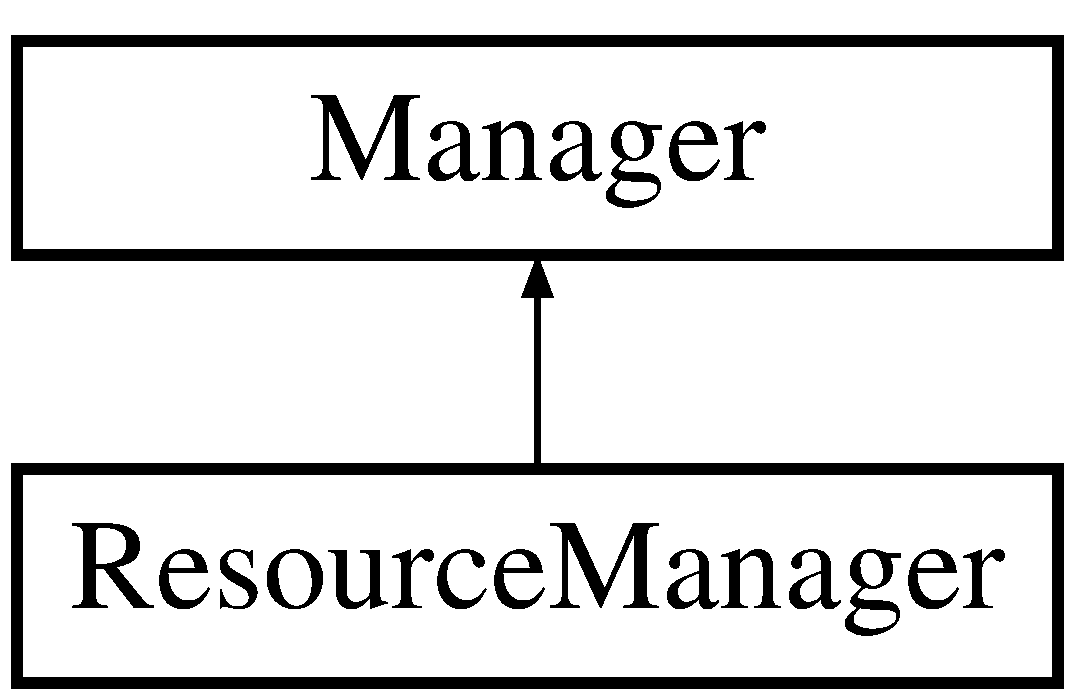
\includegraphics[height=2.000000cm]{class_resource_manager}
\end{center}
\end{figure}
\subsection*{Public Member Functions}
\begin{DoxyCompactItemize}
\item 
int \hyperlink{class_resource_manager_a53bf358b029e050a285725bc70a8550a}{start\+Up} ()
\item 
void \hyperlink{class_resource_manager_a6db779a2721e927cffb9f0c7ab31495c}{shut\+Down} ()
\item 
bool \hyperlink{class_resource_manager_aadd9ea4561168835c5c8eec0d7ff6f53}{load\+Sprite} (string file, string label)
\item 
bool \hyperlink{class_resource_manager_a6e7ab1b45dc7e6fa9abcbce827f5ddad}{unload\+Sprite} (string label)
\item 
\hyperlink{class_sprite}{Sprite} $\ast$ \hyperlink{class_resource_manager_a42c23fc9feb582cd7cc0987361ba4c6d}{get\+Sprite} (string label) const 
\end{DoxyCompactItemize}
\subsection*{Static Public Member Functions}
\begin{DoxyCompactItemize}
\item 
static \hyperlink{class_resource_manager}{Resource\+Manager} \& \hyperlink{class_resource_manager_a37d0e97686c031cef9b22725ba4a6005}{get\+Instance} ()
\end{DoxyCompactItemize}


\subsection{Detailed Description}
Handles loading and unloading resources 

\subsection{Member Function Documentation}
\hypertarget{class_resource_manager_a37d0e97686c031cef9b22725ba4a6005}{\index{Resource\+Manager@{Resource\+Manager}!get\+Instance@{get\+Instance}}
\index{get\+Instance@{get\+Instance}!Resource\+Manager@{Resource\+Manager}}
\subsubsection[{get\+Instance}]{\setlength{\rightskip}{0pt plus 5cm}{\bf Resource\+Manager} \& Resource\+Manager\+::get\+Instance (
\begin{DoxyParamCaption}
{}
\end{DoxyParamCaption}
)\hspace{0.3cm}{\ttfamily [static]}}}\label{class_resource_manager_a37d0e97686c031cef9b22725ba4a6005}
Gets the singleton instance of the resource manager \begin{DoxyReturn}{Returns}
A reference to the resource manager 
\end{DoxyReturn}
\hypertarget{class_resource_manager_a42c23fc9feb582cd7cc0987361ba4c6d}{\index{Resource\+Manager@{Resource\+Manager}!get\+Sprite@{get\+Sprite}}
\index{get\+Sprite@{get\+Sprite}!Resource\+Manager@{Resource\+Manager}}
\subsubsection[{get\+Sprite}]{\setlength{\rightskip}{0pt plus 5cm}{\bf Sprite} $\ast$ Resource\+Manager\+::get\+Sprite (
\begin{DoxyParamCaption}
\item[{string}]{label}
\end{DoxyParamCaption}
) const}}\label{class_resource_manager_a42c23fc9feb582cd7cc0987361ba4c6d}
Gets a sprite from the resource lookup table 
\begin{DoxyParams}{Parameters}
{\em label} & The label that the sprite was assigned \\
\hline
\end{DoxyParams}
\begin{DoxyReturn}{Returns}
A ptr to the sprite if the sprite was found, N\+U\+L\+L otherwise 
\end{DoxyReturn}
\hypertarget{class_resource_manager_aadd9ea4561168835c5c8eec0d7ff6f53}{\index{Resource\+Manager@{Resource\+Manager}!load\+Sprite@{load\+Sprite}}
\index{load\+Sprite@{load\+Sprite}!Resource\+Manager@{Resource\+Manager}}
\subsubsection[{load\+Sprite}]{\setlength{\rightskip}{0pt plus 5cm}bool Resource\+Manager\+::load\+Sprite (
\begin{DoxyParamCaption}
\item[{string}]{file, }
\item[{string}]{label}
\end{DoxyParamCaption}
)}}\label{class_resource_manager_aadd9ea4561168835c5c8eec0d7ff6f53}
Loads a sprite from file into memory 
\begin{DoxyParams}{Parameters}
{\em file} & The file to load from \\
\hline
{\em label} & The label to assign the sprite \\
\hline
\end{DoxyParams}
\begin{DoxyReturn}{Returns}
True if the sprite could be loaded, false otherwise 
\end{DoxyReturn}
\hypertarget{class_resource_manager_a6db779a2721e927cffb9f0c7ab31495c}{\index{Resource\+Manager@{Resource\+Manager}!shut\+Down@{shut\+Down}}
\index{shut\+Down@{shut\+Down}!Resource\+Manager@{Resource\+Manager}}
\subsubsection[{shut\+Down}]{\setlength{\rightskip}{0pt plus 5cm}void Resource\+Manager\+::shut\+Down (
\begin{DoxyParamCaption}
{}
\end{DoxyParamCaption}
)\hspace{0.3cm}{\ttfamily [virtual]}}}\label{class_resource_manager_a6db779a2721e927cffb9f0c7ab31495c}
Called when the resource manager is shut down 

Reimplemented from \hyperlink{class_manager_a09f0aaf6012be52b75a12fac25370f61}{Manager}.

\hypertarget{class_resource_manager_a53bf358b029e050a285725bc70a8550a}{\index{Resource\+Manager@{Resource\+Manager}!start\+Up@{start\+Up}}
\index{start\+Up@{start\+Up}!Resource\+Manager@{Resource\+Manager}}
\subsubsection[{start\+Up}]{\setlength{\rightskip}{0pt plus 5cm}int Resource\+Manager\+::start\+Up (
\begin{DoxyParamCaption}
{}
\end{DoxyParamCaption}
)\hspace{0.3cm}{\ttfamily [virtual]}}}\label{class_resource_manager_a53bf358b029e050a285725bc70a8550a}
Called when the resource manager is started \begin{DoxyReturn}{Returns}
0 on ok, -\/1 otherwise 
\end{DoxyReturn}


Reimplemented from \hyperlink{class_manager_a2a0f0d6810a5a051afd707d83ff1ff36}{Manager}.

\hypertarget{class_resource_manager_a6e7ab1b45dc7e6fa9abcbce827f5ddad}{\index{Resource\+Manager@{Resource\+Manager}!unload\+Sprite@{unload\+Sprite}}
\index{unload\+Sprite@{unload\+Sprite}!Resource\+Manager@{Resource\+Manager}}
\subsubsection[{unload\+Sprite}]{\setlength{\rightskip}{0pt plus 5cm}bool Resource\+Manager\+::unload\+Sprite (
\begin{DoxyParamCaption}
\item[{string}]{label}
\end{DoxyParamCaption}
)}}\label{class_resource_manager_a6e7ab1b45dc7e6fa9abcbce827f5ddad}
Unloads a sprite from memory 
\begin{DoxyParams}{Parameters}
{\em label} & The label of the sprite \\
\hline
\end{DoxyParams}
\begin{DoxyReturn}{Returns}
True if the sprite could be unloaded, false otherwise 
\end{DoxyReturn}


The documentation for this class was generated from the following files\+:\begin{DoxyCompactItemize}
\item 
F\+:/\+Users/\+Benny/git/\+I\+M\+G\+D3000/\+I\+M\+G\+D3000\+Proj3/include/Resource\+Manager.\+h\item 
F\+:/\+Users/\+Benny/git/\+I\+M\+G\+D3000/\+I\+M\+G\+D3000\+Proj3/lib/src/\+Resources/Resource\+Manager.\+cpp\end{DoxyCompactItemize}

\hypertarget{class_sprite}{\section{Sprite Class Reference}
\label{class_sprite}\index{Sprite@{Sprite}}
}


{\ttfamily \#include $<$Sprite.\+h$>$}

\subsection*{Public Member Functions}
\begin{DoxyCompactItemize}
\item 
\hyperlink{class_sprite_a613e3ce159a3a9c74a3b3ad4f94d503c}{Sprite} (string label, int frame\+Count)
\item 
string \hyperlink{class_sprite_a814ee6ee24dfefdaaa203f45c18983df}{get\+Label} () const 
\item 
int \hyperlink{class_sprite_ab9e792dcb7560a6d1af2e102bee229d6}{get\+Color} () const 
\item 
void \hyperlink{class_sprite_aa5d55e89c7e2e44122faf464987fd7a4}{set\+Color} (int color)
\item 
int \hyperlink{class_sprite_a0d3e7e4fc3123fde8bba195061c66732}{get\+Width} () const 
\item 
void \hyperlink{class_sprite_abe146a7be9978735c74b6057326e5b83}{set\+Width} (int width)
\item 
int \hyperlink{class_sprite_a526cf9f08dd1b9e39b695f224efa462f}{get\+Height} () const 
\item 
void \hyperlink{class_sprite_ac94ab494261f9e6fdb725476c8e7bf99}{set\+Height} (int height)
\item 
\hyperlink{class_frame}{Frame} $\ast$ \hyperlink{class_sprite_a37dff103a01f4820a199111039349481}{get\+Frame} (int index) const 
\item 
size\+\_\+t \hyperlink{class_sprite_a6c3c7f9caa3410f79d4711e197a159e5}{get\+Frame\+Count} () const 
\item 
bool \hyperlink{class_sprite_aa7afadb031e0c14cbd42863e445f2f9d}{add\+Frame} (\hyperlink{class_frame}{Frame} $\ast$frame)
\end{DoxyCompactItemize}


\subsection{Detailed Description}
A sprite made out of characters 

\subsection{Constructor \& Destructor Documentation}
\hypertarget{class_sprite_a613e3ce159a3a9c74a3b3ad4f94d503c}{\index{Sprite@{Sprite}!Sprite@{Sprite}}
\index{Sprite@{Sprite}!Sprite@{Sprite}}
\subsubsection[{Sprite}]{\setlength{\rightskip}{0pt plus 5cm}Sprite\+::\+Sprite (
\begin{DoxyParamCaption}
\item[{string}]{label, }
\item[{int}]{frame\+Count}
\end{DoxyParamCaption}
)}}\label{class_sprite_a613e3ce159a3a9c74a3b3ad4f94d503c}
Creates a new sprite 
\begin{DoxyParams}{Parameters}
{\em frame\+Count} & The number of frames in this sprite \\
\hline
\end{DoxyParams}


\subsection{Member Function Documentation}
\hypertarget{class_sprite_aa7afadb031e0c14cbd42863e445f2f9d}{\index{Sprite@{Sprite}!add\+Frame@{add\+Frame}}
\index{add\+Frame@{add\+Frame}!Sprite@{Sprite}}
\subsubsection[{add\+Frame}]{\setlength{\rightskip}{0pt plus 5cm}bool Sprite\+::add\+Frame (
\begin{DoxyParamCaption}
\item[{{\bf Frame} $\ast$}]{frame}
\end{DoxyParamCaption}
)}}\label{class_sprite_aa7afadb031e0c14cbd42863e445f2f9d}
Adds a frame to the sprite 
\begin{DoxyParams}{Parameters}
{\em frame} & The new frame to add \\
\hline
\end{DoxyParams}
\begin{DoxyReturn}{Returns}
True if the frame was added, false otherwise 
\end{DoxyReturn}
\hypertarget{class_sprite_ab9e792dcb7560a6d1af2e102bee229d6}{\index{Sprite@{Sprite}!get\+Color@{get\+Color}}
\index{get\+Color@{get\+Color}!Sprite@{Sprite}}
\subsubsection[{get\+Color}]{\setlength{\rightskip}{0pt plus 5cm}int Sprite\+::get\+Color (
\begin{DoxyParamCaption}
{}
\end{DoxyParamCaption}
) const}}\label{class_sprite_ab9e792dcb7560a6d1af2e102bee229d6}
Gets the color of the sprite \begin{DoxyReturn}{Returns}
The color of the sprite 
\end{DoxyReturn}
\hypertarget{class_sprite_a37dff103a01f4820a199111039349481}{\index{Sprite@{Sprite}!get\+Frame@{get\+Frame}}
\index{get\+Frame@{get\+Frame}!Sprite@{Sprite}}
\subsubsection[{get\+Frame}]{\setlength{\rightskip}{0pt plus 5cm}{\bf Frame} $\ast$ Sprite\+::get\+Frame (
\begin{DoxyParamCaption}
\item[{int}]{index}
\end{DoxyParamCaption}
) const}}\label{class_sprite_a37dff103a01f4820a199111039349481}
Get a frame in the sprite 
\begin{DoxyParams}{Parameters}
{\em index} & The index of the frame to get \\
\hline
\end{DoxyParams}
\begin{DoxyReturn}{Returns}
The frame at index, or N\+U\+L\+L if it is not found 
\end{DoxyReturn}
\hypertarget{class_sprite_a6c3c7f9caa3410f79d4711e197a159e5}{\index{Sprite@{Sprite}!get\+Frame\+Count@{get\+Frame\+Count}}
\index{get\+Frame\+Count@{get\+Frame\+Count}!Sprite@{Sprite}}
\subsubsection[{get\+Frame\+Count}]{\setlength{\rightskip}{0pt plus 5cm}size\+\_\+t Sprite\+::get\+Frame\+Count (
\begin{DoxyParamCaption}
{}
\end{DoxyParamCaption}
) const}}\label{class_sprite_a6c3c7f9caa3410f79d4711e197a159e5}
Gets the number of frames in this sprite \begin{DoxyReturn}{Returns}
The number of frames in this sprite 
\end{DoxyReturn}
\hypertarget{class_sprite_a526cf9f08dd1b9e39b695f224efa462f}{\index{Sprite@{Sprite}!get\+Height@{get\+Height}}
\index{get\+Height@{get\+Height}!Sprite@{Sprite}}
\subsubsection[{get\+Height}]{\setlength{\rightskip}{0pt plus 5cm}int Sprite\+::get\+Height (
\begin{DoxyParamCaption}
{}
\end{DoxyParamCaption}
) const}}\label{class_sprite_a526cf9f08dd1b9e39b695f224efa462f}
Sets the height of the sprite \begin{DoxyReturn}{Returns}
The height of the sprite in characters 
\end{DoxyReturn}
\hypertarget{class_sprite_a814ee6ee24dfefdaaa203f45c18983df}{\index{Sprite@{Sprite}!get\+Label@{get\+Label}}
\index{get\+Label@{get\+Label}!Sprite@{Sprite}}
\subsubsection[{get\+Label}]{\setlength{\rightskip}{0pt plus 5cm}string Sprite\+::get\+Label (
\begin{DoxyParamCaption}
{}
\end{DoxyParamCaption}
) const}}\label{class_sprite_a814ee6ee24dfefdaaa203f45c18983df}
Gets the sprites label that it is referenced by in the resource manager \begin{DoxyReturn}{Returns}

\end{DoxyReturn}
\hypertarget{class_sprite_a0d3e7e4fc3123fde8bba195061c66732}{\index{Sprite@{Sprite}!get\+Width@{get\+Width}}
\index{get\+Width@{get\+Width}!Sprite@{Sprite}}
\subsubsection[{get\+Width}]{\setlength{\rightskip}{0pt plus 5cm}int Sprite\+::get\+Width (
\begin{DoxyParamCaption}
{}
\end{DoxyParamCaption}
) const}}\label{class_sprite_a0d3e7e4fc3123fde8bba195061c66732}
Gets the width of the sprite \begin{DoxyReturn}{Returns}
The width of the sprite in characters 
\end{DoxyReturn}
\hypertarget{class_sprite_aa5d55e89c7e2e44122faf464987fd7a4}{\index{Sprite@{Sprite}!set\+Color@{set\+Color}}
\index{set\+Color@{set\+Color}!Sprite@{Sprite}}
\subsubsection[{set\+Color}]{\setlength{\rightskip}{0pt plus 5cm}void Sprite\+::set\+Color (
\begin{DoxyParamCaption}
\item[{int}]{color}
\end{DoxyParamCaption}
)}}\label{class_sprite_aa5d55e89c7e2e44122faf464987fd7a4}
Sets the color of the sprite 
\begin{DoxyParams}{Parameters}
{\em color} & The new color for the sprite \\
\hline
\end{DoxyParams}
\hypertarget{class_sprite_ac94ab494261f9e6fdb725476c8e7bf99}{\index{Sprite@{Sprite}!set\+Height@{set\+Height}}
\index{set\+Height@{set\+Height}!Sprite@{Sprite}}
\subsubsection[{set\+Height}]{\setlength{\rightskip}{0pt plus 5cm}void Sprite\+::set\+Height (
\begin{DoxyParamCaption}
\item[{int}]{height}
\end{DoxyParamCaption}
)}}\label{class_sprite_ac94ab494261f9e6fdb725476c8e7bf99}
Sets the height of the sprite 
\begin{DoxyParams}{Parameters}
{\em height} & The new height of the sprite in characters \\
\hline
\end{DoxyParams}
\hypertarget{class_sprite_abe146a7be9978735c74b6057326e5b83}{\index{Sprite@{Sprite}!set\+Width@{set\+Width}}
\index{set\+Width@{set\+Width}!Sprite@{Sprite}}
\subsubsection[{set\+Width}]{\setlength{\rightskip}{0pt plus 5cm}void Sprite\+::set\+Width (
\begin{DoxyParamCaption}
\item[{int}]{width}
\end{DoxyParamCaption}
)}}\label{class_sprite_abe146a7be9978735c74b6057326e5b83}
Sets the width of the sprite 
\begin{DoxyParams}{Parameters}
{\em width} & The new width of the sprite in characters \\
\hline
\end{DoxyParams}


The documentation for this class was generated from the following files\+:\begin{DoxyCompactItemize}
\item 
F\+:/\+Users/\+Benny/git/\+I\+M\+G\+D3000/\+I\+M\+G\+D3000\+Proj3/include/Sprite.\+h\item 
F\+:/\+Users/\+Benny/git/\+I\+M\+G\+D3000/\+I\+M\+G\+D3000\+Proj3/lib/src/\+Resources/Sprite.\+cpp\end{DoxyCompactItemize}

\hypertarget{class_sprite_object}{\section{Sprite\+Object Class Reference}
\label{class_sprite_object}\index{Sprite\+Object@{Sprite\+Object}}
}


{\ttfamily \#include $<$Sprite\+Object.\+h$>$}

Inheritance diagram for Sprite\+Object\+:\begin{figure}[H]
\begin{center}
\leavevmode
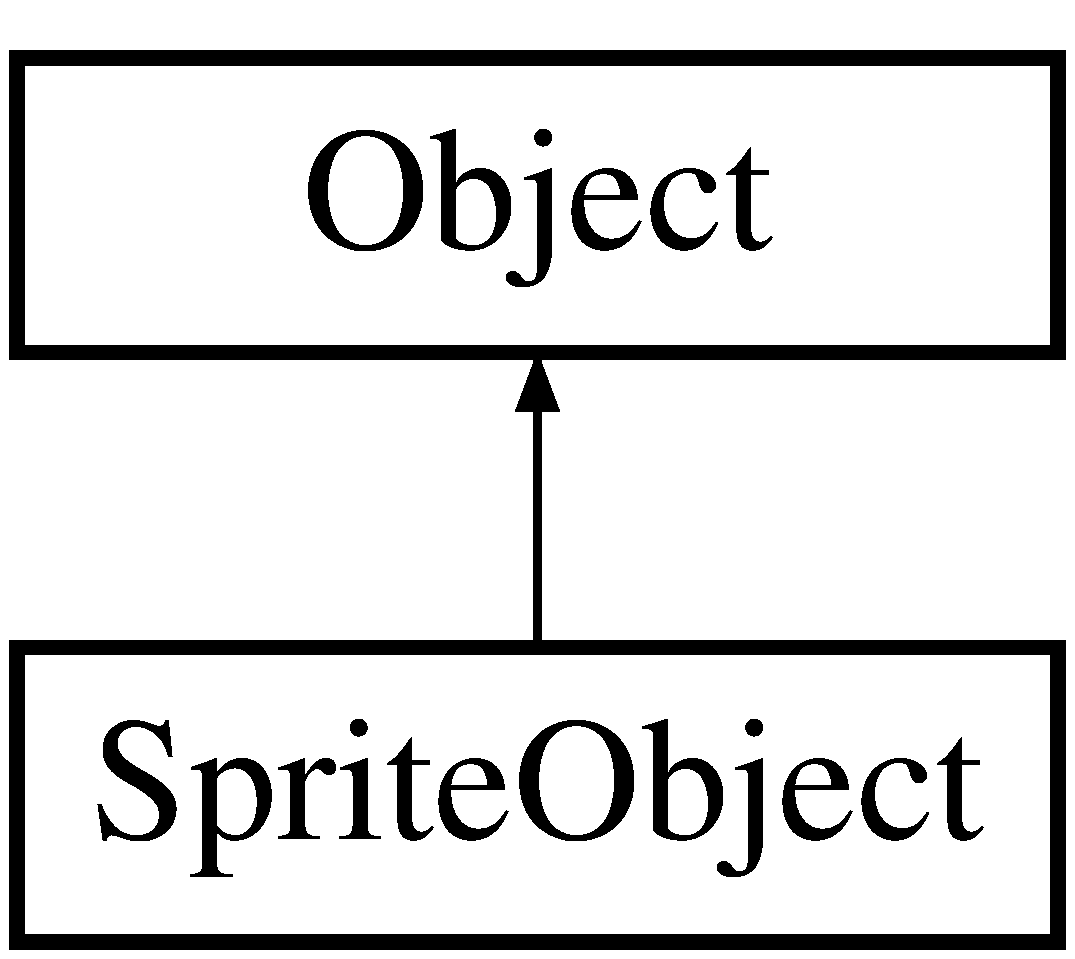
\includegraphics[height=2.000000cm]{class_sprite_object}
\end{center}
\end{figure}
\subsection*{Public Member Functions}
\begin{DoxyCompactItemize}
\item 
\hyperlink{class_sprite_object_a2f087f058dc5fcbee302a8f55c20e056}{Sprite\+Object} ()
\item 
virtual void \hyperlink{class_sprite_object_ae847b803fc182b7ff0136d902b80819a}{draw} ()
\item 
\hyperlink{class_sprite}{Sprite} $\ast$ \hyperlink{class_sprite_object_a6e08d86800af64b64f418675ee6e453c}{get\+Sprite} () const 
\item 
void \hyperlink{class_sprite_object_a5898d37e753a73122c7b4364acd1586d}{set\+Sprite} (\hyperlink{class_sprite}{Sprite} $\ast$sprite, bool set\+Box=true)
\item 
bool \hyperlink{class_sprite_object_a945f4ca943003fc34b8bb36e42d77510}{is\+Centered} () const 
\item 
void \hyperlink{class_sprite_object_aa27b75d323d453069433dbaa39e5df85}{set\+Centered} (bool centered)
\item 
void \hyperlink{class_sprite_object_a2d43271a2ab04e28a358b7e13d8f9d17}{set\+Frame\+Index} (int frame)
\item 
int \hyperlink{class_sprite_object_a67fdbbec2ebbabe75274143e2d05c86b}{get\+Frame\+Index} () const 
\item 
void \hyperlink{class_sprite_object_a4a128cde5497bc293b301d9faeffe4f6}{set\+Slowdown} (int slowdown)
\item 
int \hyperlink{class_sprite_object_af815a869de3942821121c7c8369037b2}{get\+Slowdown} () const 
\end{DoxyCompactItemize}


\subsection{Detailed Description}
\hyperlink{class_object}{Object} that can display a sprite to the screen 

\subsection{Constructor \& Destructor Documentation}
\hypertarget{class_sprite_object_a2f087f058dc5fcbee302a8f55c20e056}{\index{Sprite\+Object@{Sprite\+Object}!Sprite\+Object@{Sprite\+Object}}
\index{Sprite\+Object@{Sprite\+Object}!Sprite\+Object@{Sprite\+Object}}
\subsubsection[{Sprite\+Object}]{\setlength{\rightskip}{0pt plus 5cm}Sprite\+Object\+::\+Sprite\+Object (
\begin{DoxyParamCaption}
{}
\end{DoxyParamCaption}
)}}\label{class_sprite_object_a2f087f058dc5fcbee302a8f55c20e056}
Creates a default sprite object 

\subsection{Member Function Documentation}
\hypertarget{class_sprite_object_ae847b803fc182b7ff0136d902b80819a}{\index{Sprite\+Object@{Sprite\+Object}!draw@{draw}}
\index{draw@{draw}!Sprite\+Object@{Sprite\+Object}}
\subsubsection[{draw}]{\setlength{\rightskip}{0pt plus 5cm}void Sprite\+Object\+::draw (
\begin{DoxyParamCaption}
{}
\end{DoxyParamCaption}
)\hspace{0.3cm}{\ttfamily [virtual]}}}\label{class_sprite_object_ae847b803fc182b7ff0136d902b80819a}
Called once per frame to draw the object 

Reimplemented from \hyperlink{class_object_a821f5b25b450fa1acdb3f9c0b5962592}{Object}.

\hypertarget{class_sprite_object_a67fdbbec2ebbabe75274143e2d05c86b}{\index{Sprite\+Object@{Sprite\+Object}!get\+Frame\+Index@{get\+Frame\+Index}}
\index{get\+Frame\+Index@{get\+Frame\+Index}!Sprite\+Object@{Sprite\+Object}}
\subsubsection[{get\+Frame\+Index}]{\setlength{\rightskip}{0pt plus 5cm}int Sprite\+Object\+::get\+Frame\+Index (
\begin{DoxyParamCaption}
{}
\end{DoxyParamCaption}
) const}}\label{class_sprite_object_a67fdbbec2ebbabe75274143e2d05c86b}
Gets the index of the current frame of the sprite \begin{DoxyReturn}{Returns}
The index of the current frame 
\end{DoxyReturn}
\hypertarget{class_sprite_object_af815a869de3942821121c7c8369037b2}{\index{Sprite\+Object@{Sprite\+Object}!get\+Slowdown@{get\+Slowdown}}
\index{get\+Slowdown@{get\+Slowdown}!Sprite\+Object@{Sprite\+Object}}
\subsubsection[{get\+Slowdown}]{\setlength{\rightskip}{0pt plus 5cm}int Sprite\+Object\+::get\+Slowdown (
\begin{DoxyParamCaption}
{}
\end{DoxyParamCaption}
) const}}\label{class_sprite_object_af815a869de3942821121c7c8369037b2}
Gets the slowdown for the animation \begin{DoxyReturn}{Returns}
The number of frames to wait before drawing the next frame 
\end{DoxyReturn}
\hypertarget{class_sprite_object_a6e08d86800af64b64f418675ee6e453c}{\index{Sprite\+Object@{Sprite\+Object}!get\+Sprite@{get\+Sprite}}
\index{get\+Sprite@{get\+Sprite}!Sprite\+Object@{Sprite\+Object}}
\subsubsection[{get\+Sprite}]{\setlength{\rightskip}{0pt plus 5cm}{\bf Sprite} $\ast$ Sprite\+Object\+::get\+Sprite (
\begin{DoxyParamCaption}
{}
\end{DoxyParamCaption}
) const}}\label{class_sprite_object_a6e08d86800af64b64f418675ee6e453c}
Gets the sprite that this object uses \begin{DoxyReturn}{Returns}
The sprite this object uses or N\+U\+L\+L if there is none 
\end{DoxyReturn}
\hypertarget{class_sprite_object_a945f4ca943003fc34b8bb36e42d77510}{\index{Sprite\+Object@{Sprite\+Object}!is\+Centered@{is\+Centered}}
\index{is\+Centered@{is\+Centered}!Sprite\+Object@{Sprite\+Object}}
\subsubsection[{is\+Centered}]{\setlength{\rightskip}{0pt plus 5cm}bool Sprite\+Object\+::is\+Centered (
\begin{DoxyParamCaption}
{}
\end{DoxyParamCaption}
) const}}\label{class_sprite_object_a945f4ca943003fc34b8bb36e42d77510}
Checks to see if this object is centered on its position \begin{DoxyReturn}{Returns}
True if it is centered, false otherwise 
\end{DoxyReturn}
\hypertarget{class_sprite_object_aa27b75d323d453069433dbaa39e5df85}{\index{Sprite\+Object@{Sprite\+Object}!set\+Centered@{set\+Centered}}
\index{set\+Centered@{set\+Centered}!Sprite\+Object@{Sprite\+Object}}
\subsubsection[{set\+Centered}]{\setlength{\rightskip}{0pt plus 5cm}void Sprite\+Object\+::set\+Centered (
\begin{DoxyParamCaption}
\item[{bool}]{centered}
\end{DoxyParamCaption}
)}}\label{class_sprite_object_aa27b75d323d453069433dbaa39e5df85}
Sets if this object should be centered on its world position or not 
\begin{DoxyParams}{Parameters}
{\em centered} & If true the object will be centered, if false the object will not \\
\hline
\end{DoxyParams}
\hypertarget{class_sprite_object_a2d43271a2ab04e28a358b7e13d8f9d17}{\index{Sprite\+Object@{Sprite\+Object}!set\+Frame\+Index@{set\+Frame\+Index}}
\index{set\+Frame\+Index@{set\+Frame\+Index}!Sprite\+Object@{Sprite\+Object}}
\subsubsection[{set\+Frame\+Index}]{\setlength{\rightskip}{0pt plus 5cm}void Sprite\+Object\+::set\+Frame\+Index (
\begin{DoxyParamCaption}
\item[{int}]{frame}
\end{DoxyParamCaption}
)}}\label{class_sprite_object_a2d43271a2ab04e28a358b7e13d8f9d17}
Sets the current frame that the object should render 
\begin{DoxyParams}{Parameters}
{\em frame} & The index of the frame in the sprite, if this number is out of bounds it will be wrapped around to fit \\
\hline
\end{DoxyParams}
\hypertarget{class_sprite_object_a4a128cde5497bc293b301d9faeffe4f6}{\index{Sprite\+Object@{Sprite\+Object}!set\+Slowdown@{set\+Slowdown}}
\index{set\+Slowdown@{set\+Slowdown}!Sprite\+Object@{Sprite\+Object}}
\subsubsection[{set\+Slowdown}]{\setlength{\rightskip}{0pt plus 5cm}void Sprite\+Object\+::set\+Slowdown (
\begin{DoxyParamCaption}
\item[{int}]{slowdown}
\end{DoxyParamCaption}
)}}\label{class_sprite_object_a4a128cde5497bc293b301d9faeffe4f6}
Sets the slowdown on the animation 
\begin{DoxyParams}{Parameters}
{\em slowdown} & The number of frames to wait before drawing the next frame \\
\hline
\end{DoxyParams}
\hypertarget{class_sprite_object_a5898d37e753a73122c7b4364acd1586d}{\index{Sprite\+Object@{Sprite\+Object}!set\+Sprite@{set\+Sprite}}
\index{set\+Sprite@{set\+Sprite}!Sprite\+Object@{Sprite\+Object}}
\subsubsection[{set\+Sprite}]{\setlength{\rightskip}{0pt plus 5cm}void Sprite\+Object\+::set\+Sprite (
\begin{DoxyParamCaption}
\item[{{\bf Sprite} $\ast$}]{sprite, }
\item[{bool}]{set\+Box = {\ttfamily true}}
\end{DoxyParamCaption}
)}}\label{class_sprite_object_a5898d37e753a73122c7b4364acd1586d}
Sets the sprite for this object 
\begin{DoxyParams}{Parameters}
{\em sprite} & The sprite that this object should use \\
\hline
{\em set\+Box} & If true then the bounding box for this object will be set to fit this sprite \\
\hline
\end{DoxyParams}


The documentation for this class was generated from the following files\+:\begin{DoxyCompactItemize}
\item 
F\+:/\+Users/\+Benny/git/\+I\+M\+G\+D3000/\+I\+M\+G\+D3000\+Proj3/include/Sprite\+Object.\+h\item 
F\+:/\+Users/\+Benny/git/\+I\+M\+G\+D3000/\+I\+M\+G\+D3000\+Proj3/lib/src/\+Object/Sprite\+Object.\+cpp\end{DoxyCompactItemize}

\hypertarget{class_status_bar}{\section{Status\+Bar Class Reference}
\label{class_status_bar}\index{Status\+Bar@{Status\+Bar}}
}


{\ttfamily \#include $<$Status\+Bar.\+h$>$}

Inheritance diagram for Status\+Bar\+:\begin{figure}[H]
\begin{center}
\leavevmode
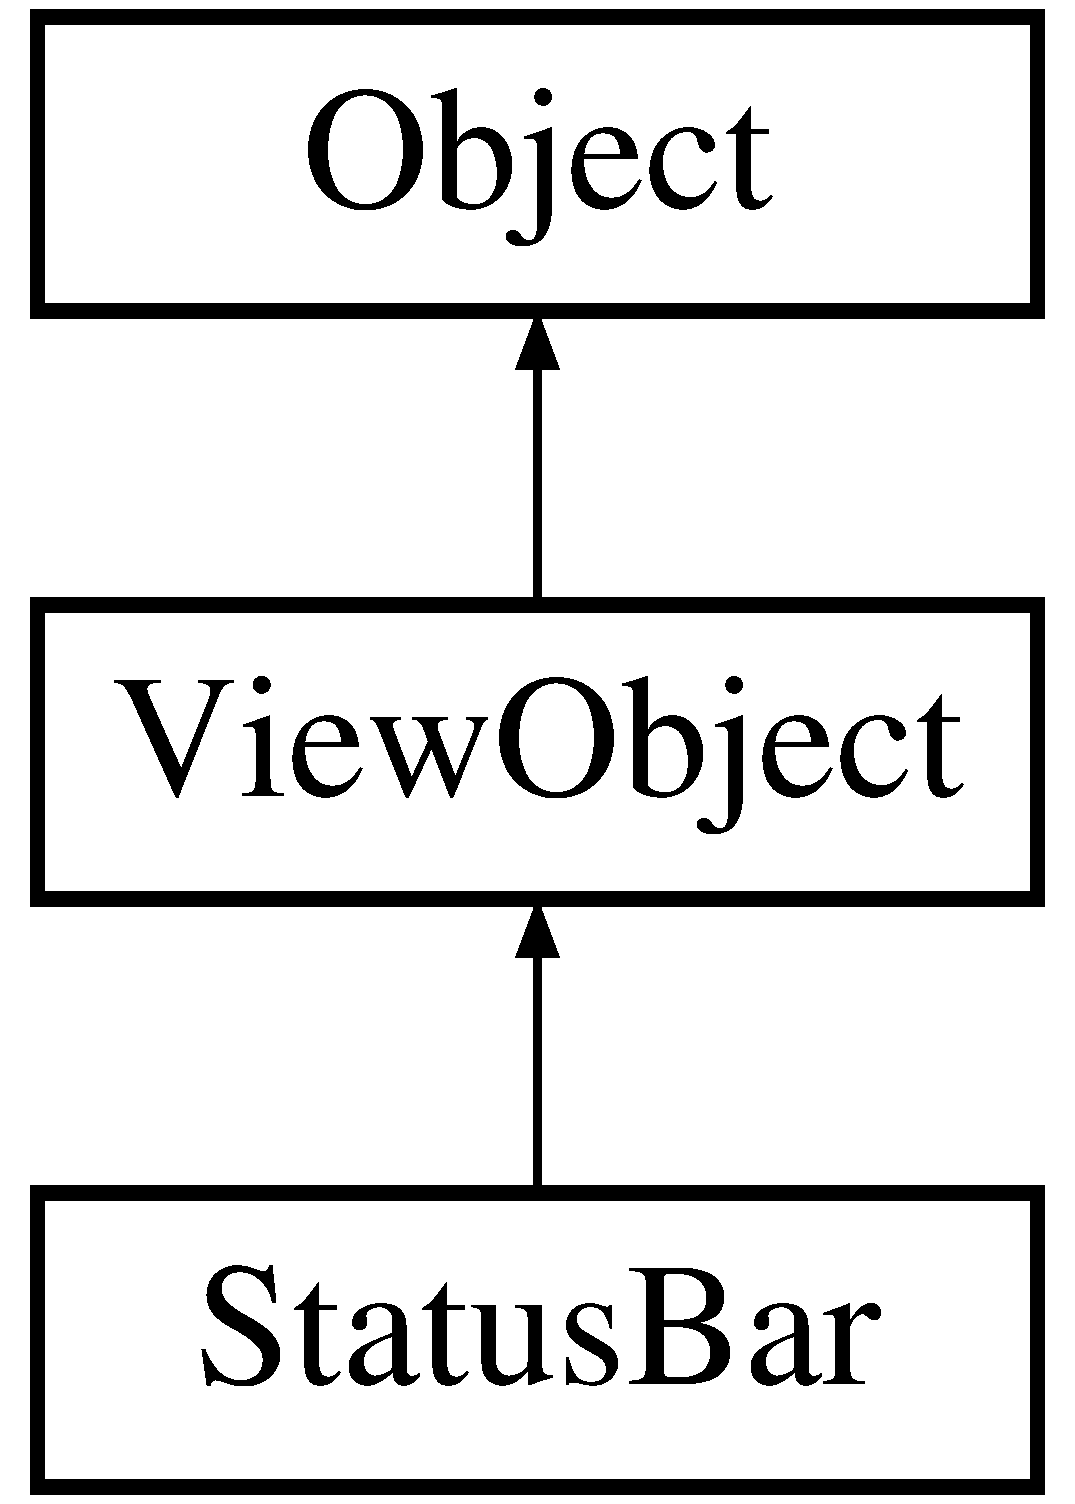
\includegraphics[height=3.000000cm]{class_status_bar}
\end{center}
\end{figure}
\subsection*{Public Member Functions}
\begin{DoxyCompactItemize}
\item 
\hyperlink{class_status_bar_a651573f47ad4106ceb73c125685116c8}{Status\+Bar} (int max\+Value)
\end{DoxyCompactItemize}
\subsection*{Protected Member Functions}
\begin{DoxyCompactItemize}
\item 
virtual string \hyperlink{class_status_bar_a3213353214665edfaa66eead5af8ea27}{get\+Render\+String} () const 
\end{DoxyCompactItemize}


\subsection{Detailed Description}
Renders a value as a bar 

\subsection{Constructor \& Destructor Documentation}
\hypertarget{class_status_bar_a651573f47ad4106ceb73c125685116c8}{\index{Status\+Bar@{Status\+Bar}!Status\+Bar@{Status\+Bar}}
\index{Status\+Bar@{Status\+Bar}!Status\+Bar@{Status\+Bar}}
\subsubsection[{Status\+Bar}]{\setlength{\rightskip}{0pt plus 5cm}Status\+Bar\+::\+Status\+Bar (
\begin{DoxyParamCaption}
\item[{int}]{max\+Value}
\end{DoxyParamCaption}
)}}\label{class_status_bar_a651573f47ad4106ceb73c125685116c8}
Creates a new status bar 
\begin{DoxyParams}{Parameters}
{\em max\+Value} & The max value for the bar \\
\hline
\end{DoxyParams}


\subsection{Member Function Documentation}
\hypertarget{class_status_bar_a3213353214665edfaa66eead5af8ea27}{\index{Status\+Bar@{Status\+Bar}!get\+Render\+String@{get\+Render\+String}}
\index{get\+Render\+String@{get\+Render\+String}!Status\+Bar@{Status\+Bar}}
\subsubsection[{get\+Render\+String}]{\setlength{\rightskip}{0pt plus 5cm}string Status\+Bar\+::get\+Render\+String (
\begin{DoxyParamCaption}
{}
\end{DoxyParamCaption}
) const\hspace{0.3cm}{\ttfamily [protected]}, {\ttfamily [virtual]}}}\label{class_status_bar_a3213353214665edfaa66eead5af8ea27}
The string to render to the scene \begin{DoxyReturn}{Returns}
The bar name followed by the bar 
\end{DoxyReturn}


Reimplemented from \hyperlink{class_view_object_a4dbdd0c17f18ff9412eaff095ab583d3}{View\+Object}.



The documentation for this class was generated from the following files\+:\begin{DoxyCompactItemize}
\item 
F\+:/\+Users/\+Benny/git/\+I\+M\+G\+D3000/\+I\+M\+G\+D3000\+Proj3/include/Status\+Bar.\+h\item 
F\+:/\+Users/\+Benny/git/\+I\+M\+G\+D3000/\+I\+M\+G\+D3000\+Proj3/lib/src/\+U\+I/Status\+Bar.\+cpp\end{DoxyCompactItemize}

\hypertarget{class_string_ptr_pair}{\section{String\+Ptr\+Pair Class Reference}
\label{class_string_ptr_pair}\index{String\+Ptr\+Pair@{String\+Ptr\+Pair}}
}


{\ttfamily \#include $<$String\+Ptr\+Pair.\+h$>$}

\subsection*{Public Member Functions}
\begin{DoxyCompactItemize}
\item 
\hyperlink{class_string_ptr_pair_ac4168e080e2704e725a0ea74b33f40e1}{String\+Ptr\+Pair} (string key, void $\ast$value)
\item 
string \hyperlink{class_string_ptr_pair_ad3262ee11668ccaa566968dc2ab956d1}{get\+Key} () const 
\item 
void $\ast$ \hyperlink{class_string_ptr_pair_addba9e1b5ba7d9da763f9025d1867673}{get\+Value} () const 
\item 
void \hyperlink{class_string_ptr_pair_aac521d7da4a5dbdeaeb9cc577f778e2e}{set\+Value} (void $\ast$value)
\end{DoxyCompactItemize}


\subsection{Detailed Description}
A key value pair that uses strings for the key and pointers for the values 

\subsection{Constructor \& Destructor Documentation}
\hypertarget{class_string_ptr_pair_ac4168e080e2704e725a0ea74b33f40e1}{\index{String\+Ptr\+Pair@{String\+Ptr\+Pair}!String\+Ptr\+Pair@{String\+Ptr\+Pair}}
\index{String\+Ptr\+Pair@{String\+Ptr\+Pair}!String\+Ptr\+Pair@{String\+Ptr\+Pair}}
\subsubsection[{String\+Ptr\+Pair}]{\setlength{\rightskip}{0pt plus 5cm}String\+Ptr\+Pair\+::\+String\+Ptr\+Pair (
\begin{DoxyParamCaption}
\item[{string}]{key, }
\item[{void $\ast$}]{value}
\end{DoxyParamCaption}
)}}\label{class_string_ptr_pair_ac4168e080e2704e725a0ea74b33f40e1}
Creates a new key value pair 
\begin{DoxyParams}{Parameters}
{\em key} & The key \\
\hline
{\em value} & The value \\
\hline
\end{DoxyParams}


\subsection{Member Function Documentation}
\hypertarget{class_string_ptr_pair_ad3262ee11668ccaa566968dc2ab956d1}{\index{String\+Ptr\+Pair@{String\+Ptr\+Pair}!get\+Key@{get\+Key}}
\index{get\+Key@{get\+Key}!String\+Ptr\+Pair@{String\+Ptr\+Pair}}
\subsubsection[{get\+Key}]{\setlength{\rightskip}{0pt plus 5cm}string String\+Ptr\+Pair\+::get\+Key (
\begin{DoxyParamCaption}
{}
\end{DoxyParamCaption}
) const}}\label{class_string_ptr_pair_ad3262ee11668ccaa566968dc2ab956d1}
Gets the key of this pair \begin{DoxyReturn}{Returns}
A string that is the key for this pair 
\end{DoxyReturn}
\hypertarget{class_string_ptr_pair_addba9e1b5ba7d9da763f9025d1867673}{\index{String\+Ptr\+Pair@{String\+Ptr\+Pair}!get\+Value@{get\+Value}}
\index{get\+Value@{get\+Value}!String\+Ptr\+Pair@{String\+Ptr\+Pair}}
\subsubsection[{get\+Value}]{\setlength{\rightskip}{0pt plus 5cm}void $\ast$ String\+Ptr\+Pair\+::get\+Value (
\begin{DoxyParamCaption}
{}
\end{DoxyParamCaption}
) const}}\label{class_string_ptr_pair_addba9e1b5ba7d9da763f9025d1867673}
Gets the value for this pair \begin{DoxyReturn}{Returns}
The value in this pair 
\end{DoxyReturn}
\hypertarget{class_string_ptr_pair_aac521d7da4a5dbdeaeb9cc577f778e2e}{\index{String\+Ptr\+Pair@{String\+Ptr\+Pair}!set\+Value@{set\+Value}}
\index{set\+Value@{set\+Value}!String\+Ptr\+Pair@{String\+Ptr\+Pair}}
\subsubsection[{set\+Value}]{\setlength{\rightskip}{0pt plus 5cm}void String\+Ptr\+Pair\+::set\+Value (
\begin{DoxyParamCaption}
\item[{void $\ast$}]{value}
\end{DoxyParamCaption}
)}}\label{class_string_ptr_pair_aac521d7da4a5dbdeaeb9cc577f778e2e}
Changes the value in this key value pair 
\begin{DoxyParams}{Parameters}
{\em value} & The new value to set the pair to \\
\hline
\end{DoxyParams}


The documentation for this class was generated from the following files\+:\begin{DoxyCompactItemize}
\item 
F\+:/\+Users/\+Benny/git/\+I\+M\+G\+D3000/\+I\+M\+G\+D3000\+Proj3/lib/src/\+Core/String\+Ptr\+Pair.\+h\item 
F\+:/\+Users/\+Benny/git/\+I\+M\+G\+D3000/\+I\+M\+G\+D3000\+Proj3/lib/src/\+Core/String\+Ptr\+Pair.\+cpp\end{DoxyCompactItemize}

\hypertarget{class_view_object}{\section{View\+Object Class Reference}
\label{class_view_object}\index{View\+Object@{View\+Object}}
}
Inheritance diagram for View\+Object\+:\begin{figure}[H]
\begin{center}
\leavevmode
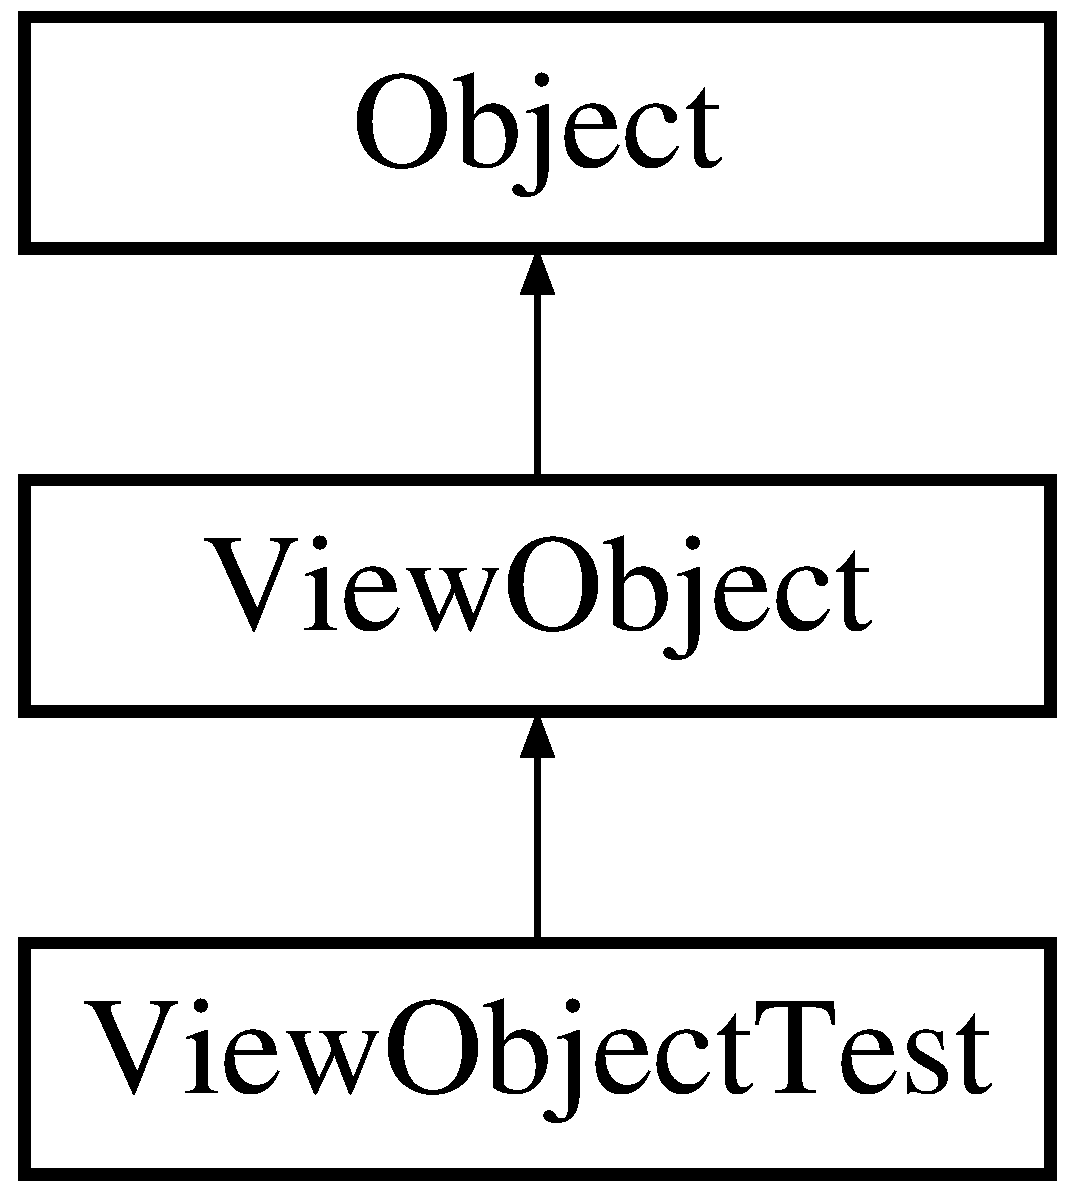
\includegraphics[height=3.000000cm]{class_view_object}
\end{center}
\end{figure}
\subsection*{Public Member Functions}
\begin{DoxyCompactItemize}
\item 
virtual int \hyperlink{class_view_object_aae06f1481afddf829a97b045a0c60bb7}{event\+Handler} (\hyperlink{class_event}{Event} $\ast$e)
\item 
virtual void \hyperlink{class_view_object_aae76e90e25d65e34d80e468b41af95da}{draw} ()
\item 
string \hyperlink{class_view_object_aca2716919c8e5cad80898a7f9962ddcc}{get\+View\+String} () const 
\item 
void \hyperlink{class_view_object_adae1f08a437032a52db37a6b7e84d046}{set\+View\+String} (string view\+String)
\item 
int \hyperlink{class_view_object_a87877b05cb9a8d44a77dc173b7738d62}{get\+Value} () const 
\item 
void \hyperlink{class_view_object_a7b6c99fea863c7eac45cbe8fcff03d96}{set\+Value} (int value)
\item 
bool \hyperlink{class_view_object_a2ba768ed1d2301a8cc06531854462078}{get\+Draw\+Border} () const 
\item 
void \hyperlink{class_view_object_a19e870c7720b8174e8293a8287d111a2}{set\+Draw\+Border} (bool draw\+Border)
\item 
Justification \hyperlink{class_view_object_a02a8ccd6e642e1f3274f1c8523c992d4}{get\+Justification} () const 
\item 
void \hyperlink{class_view_object_a48b915f41e561fd210ea5e22d690aa10}{set\+Justification} (Justification justification)
\item 
View\+Object\+Location \hyperlink{class_view_object_ac0672505b7a72ec0a4be8f261bcffe5c}{get\+View\+Object\+Location} () const 
\item 
void \hyperlink{class_view_object_a2a3ae5cb263ecc0597d1b0cc85c0300e}{set\+View\+Object\+Location} (View\+Object\+Location)
\end{DoxyCompactItemize}
\subsection*{Protected Member Functions}
\begin{DoxyCompactItemize}
\item 
virtual string \hyperlink{class_view_object_a4dbdd0c17f18ff9412eaff095ab583d3}{get\+Render\+String} () const 
\end{DoxyCompactItemize}


\subsection{Member Function Documentation}
\hypertarget{class_view_object_aae76e90e25d65e34d80e468b41af95da}{\index{View\+Object@{View\+Object}!draw@{draw}}
\index{draw@{draw}!View\+Object@{View\+Object}}
\subsubsection[{draw}]{\setlength{\rightskip}{0pt plus 5cm}void View\+Object\+::draw (
\begin{DoxyParamCaption}
{}
\end{DoxyParamCaption}
)\hspace{0.3cm}{\ttfamily [virtual]}}}\label{class_view_object_aae76e90e25d65e34d80e468b41af95da}
Called every frame when the view object is drawn 

Reimplemented from \hyperlink{class_object_a821f5b25b450fa1acdb3f9c0b5962592}{Object}.

\hypertarget{class_view_object_aae06f1481afddf829a97b045a0c60bb7}{\index{View\+Object@{View\+Object}!event\+Handler@{event\+Handler}}
\index{event\+Handler@{event\+Handler}!View\+Object@{View\+Object}}
\subsubsection[{event\+Handler}]{\setlength{\rightskip}{0pt plus 5cm}int View\+Object\+::event\+Handler (
\begin{DoxyParamCaption}
\item[{{\bf Event} $\ast$}]{e}
\end{DoxyParamCaption}
)\hspace{0.3cm}{\ttfamily [virtual]}}}\label{class_view_object_aae06f1481afddf829a97b045a0c60bb7}
Handles events given to this object 
\begin{DoxyParams}{Parameters}
{\em e} & A pointer to the event data \\
\hline
\end{DoxyParams}
\begin{DoxyReturn}{Returns}
a non-\/zero number if this object does consume the event, otherwise 0 
\end{DoxyReturn}


Reimplemented from \hyperlink{class_object_aef5d6ac71c5184a72e7101584d377998}{Object}.

\hypertarget{class_view_object_a2ba768ed1d2301a8cc06531854462078}{\index{View\+Object@{View\+Object}!get\+Draw\+Border@{get\+Draw\+Border}}
\index{get\+Draw\+Border@{get\+Draw\+Border}!View\+Object@{View\+Object}}
\subsubsection[{get\+Draw\+Border}]{\setlength{\rightskip}{0pt plus 5cm}bool View\+Object\+::get\+Draw\+Border (
\begin{DoxyParamCaption}
{}
\end{DoxyParamCaption}
) const}}\label{class_view_object_a2ba768ed1d2301a8cc06531854462078}
Gets if we are drawing a border on this object \begin{DoxyReturn}{Returns}
True if we are drawing a border, false otherwise 
\end{DoxyReturn}
\hypertarget{class_view_object_a02a8ccd6e642e1f3274f1c8523c992d4}{\index{View\+Object@{View\+Object}!get\+Justification@{get\+Justification}}
\index{get\+Justification@{get\+Justification}!View\+Object@{View\+Object}}
\subsubsection[{get\+Justification}]{\setlength{\rightskip}{0pt plus 5cm}Justification View\+Object\+::get\+Justification (
\begin{DoxyParamCaption}
{}
\end{DoxyParamCaption}
) const}}\label{class_view_object_a02a8ccd6e642e1f3274f1c8523c992d4}
Gets the justification on the string that is going to be drawn \begin{DoxyReturn}{Returns}
The justification on the string 
\end{DoxyReturn}
\hypertarget{class_view_object_a4dbdd0c17f18ff9412eaff095ab583d3}{\index{View\+Object@{View\+Object}!get\+Render\+String@{get\+Render\+String}}
\index{get\+Render\+String@{get\+Render\+String}!View\+Object@{View\+Object}}
\subsubsection[{get\+Render\+String}]{\setlength{\rightskip}{0pt plus 5cm}string View\+Object\+::get\+Render\+String (
\begin{DoxyParamCaption}
{}
\end{DoxyParamCaption}
) const\hspace{0.3cm}{\ttfamily [protected]}, {\ttfamily [virtual]}}}\label{class_view_object_a4dbdd0c17f18ff9412eaff095ab583d3}
Gets the string to be rendered \begin{DoxyReturn}{Returns}
The string to render on screen (this does not include the border 
\end{DoxyReturn}


Reimplemented in \hyperlink{class_status_bar_a3213353214665edfaa66eead5af8ea27}{Status\+Bar}.

\hypertarget{class_view_object_a87877b05cb9a8d44a77dc173b7738d62}{\index{View\+Object@{View\+Object}!get\+Value@{get\+Value}}
\index{get\+Value@{get\+Value}!View\+Object@{View\+Object}}
\subsubsection[{get\+Value}]{\setlength{\rightskip}{0pt plus 5cm}int View\+Object\+::get\+Value (
\begin{DoxyParamCaption}
{}
\end{DoxyParamCaption}
) const}}\label{class_view_object_a87877b05cb9a8d44a77dc173b7738d62}
Get the value to display \begin{DoxyReturn}{Returns}
The value to display 
\end{DoxyReturn}
\hypertarget{class_view_object_ac0672505b7a72ec0a4be8f261bcffe5c}{\index{View\+Object@{View\+Object}!get\+View\+Object\+Location@{get\+View\+Object\+Location}}
\index{get\+View\+Object\+Location@{get\+View\+Object\+Location}!View\+Object@{View\+Object}}
\subsubsection[{get\+View\+Object\+Location}]{\setlength{\rightskip}{0pt plus 5cm}View\+Object\+Location View\+Object\+::get\+View\+Object\+Location (
\begin{DoxyParamCaption}
{}
\end{DoxyParamCaption}
) const}}\label{class_view_object_ac0672505b7a72ec0a4be8f261bcffe5c}
Gets the view objects relative location on screen \begin{DoxyReturn}{Returns}
The view objects relative location on screen 
\end{DoxyReturn}
\hypertarget{class_view_object_aca2716919c8e5cad80898a7f9962ddcc}{\index{View\+Object@{View\+Object}!get\+View\+String@{get\+View\+String}}
\index{get\+View\+String@{get\+View\+String}!View\+Object@{View\+Object}}
\subsubsection[{get\+View\+String}]{\setlength{\rightskip}{0pt plus 5cm}string View\+Object\+::get\+View\+String (
\begin{DoxyParamCaption}
{}
\end{DoxyParamCaption}
) const}}\label{class_view_object_aca2716919c8e5cad80898a7f9962ddcc}
Get the string to display \begin{DoxyReturn}{Returns}
The string that will be displayed next to the value 
\end{DoxyReturn}
\hypertarget{class_view_object_a19e870c7720b8174e8293a8287d111a2}{\index{View\+Object@{View\+Object}!set\+Draw\+Border@{set\+Draw\+Border}}
\index{set\+Draw\+Border@{set\+Draw\+Border}!View\+Object@{View\+Object}}
\subsubsection[{set\+Draw\+Border}]{\setlength{\rightskip}{0pt plus 5cm}void View\+Object\+::set\+Draw\+Border (
\begin{DoxyParamCaption}
\item[{bool}]{draw\+Border}
\end{DoxyParamCaption}
)}}\label{class_view_object_a19e870c7720b8174e8293a8287d111a2}
Sets if we are drawing a border on this object 
\begin{DoxyParams}{Parameters}
{\em draw\+Border} & If true then a border will be draw, otherwise a border will not be drawn \\
\hline
\end{DoxyParams}
\hypertarget{class_view_object_a48b915f41e561fd210ea5e22d690aa10}{\index{View\+Object@{View\+Object}!set\+Justification@{set\+Justification}}
\index{set\+Justification@{set\+Justification}!View\+Object@{View\+Object}}
\subsubsection[{set\+Justification}]{\setlength{\rightskip}{0pt plus 5cm}void View\+Object\+::set\+Justification (
\begin{DoxyParamCaption}
\item[{Justification}]{justification}
\end{DoxyParamCaption}
)}}\label{class_view_object_a48b915f41e561fd210ea5e22d690aa10}
Sets the justification on the string that is being drawn 
\begin{DoxyParams}{Parameters}
{\em justification} & The justification on the string being drawn \\
\hline
\end{DoxyParams}
\hypertarget{class_view_object_a7b6c99fea863c7eac45cbe8fcff03d96}{\index{View\+Object@{View\+Object}!set\+Value@{set\+Value}}
\index{set\+Value@{set\+Value}!View\+Object@{View\+Object}}
\subsubsection[{set\+Value}]{\setlength{\rightskip}{0pt plus 5cm}void View\+Object\+::set\+Value (
\begin{DoxyParamCaption}
\item[{int}]{value}
\end{DoxyParamCaption}
)}}\label{class_view_object_a7b6c99fea863c7eac45cbe8fcff03d96}
Set the value to display 
\begin{DoxyParams}{Parameters}
{\em value} & The new value to display \\
\hline
\end{DoxyParams}
\hypertarget{class_view_object_a2a3ae5cb263ecc0597d1b0cc85c0300e}{\index{View\+Object@{View\+Object}!set\+View\+Object\+Location@{set\+View\+Object\+Location}}
\index{set\+View\+Object\+Location@{set\+View\+Object\+Location}!View\+Object@{View\+Object}}
\subsubsection[{set\+View\+Object\+Location}]{\setlength{\rightskip}{0pt plus 5cm}void View\+Object\+::set\+View\+Object\+Location (
\begin{DoxyParamCaption}
\item[{View\+Object\+Location}]{enum\+View\+Object\+Location}
\end{DoxyParamCaption}
)}}\label{class_view_object_a2a3ae5cb263ecc0597d1b0cc85c0300e}
The view objects relative location on screen 
\begin{DoxyParams}{Parameters}
{\em The} & view objects relative location on screen \\
\hline
\end{DoxyParams}
\hypertarget{class_view_object_adae1f08a437032a52db37a6b7e84d046}{\index{View\+Object@{View\+Object}!set\+View\+String@{set\+View\+String}}
\index{set\+View\+String@{set\+View\+String}!View\+Object@{View\+Object}}
\subsubsection[{set\+View\+String}]{\setlength{\rightskip}{0pt plus 5cm}void View\+Object\+::set\+View\+String (
\begin{DoxyParamCaption}
\item[{string}]{view\+String}
\end{DoxyParamCaption}
)}}\label{class_view_object_adae1f08a437032a52db37a6b7e84d046}
Sets the string to display 
\begin{DoxyParams}{Parameters}
{\em view\+String} & The new string to display next to the value \\
\hline
\end{DoxyParams}


The documentation for this class was generated from the following files\+:\begin{DoxyCompactItemize}
\item 
F\+:/\+Users/\+Benny/git/\+I\+M\+G\+D3000/\+I\+M\+G\+D3000\+Proj3/include/View\+Object.\+h\item 
F\+:/\+Users/\+Benny/git/\+I\+M\+G\+D3000/\+I\+M\+G\+D3000\+Proj3/lib/src/\+U\+I/View\+Object.\+cpp\end{DoxyCompactItemize}

\hypertarget{class_world_manager}{\section{World\+Manager Class Reference}
\label{class_world_manager}\index{World\+Manager@{World\+Manager}}
}


{\ttfamily \#include $<$World\+Manager.\+h$>$}

Inheritance diagram for World\+Manager\+:\begin{figure}[H]
\begin{center}
\leavevmode
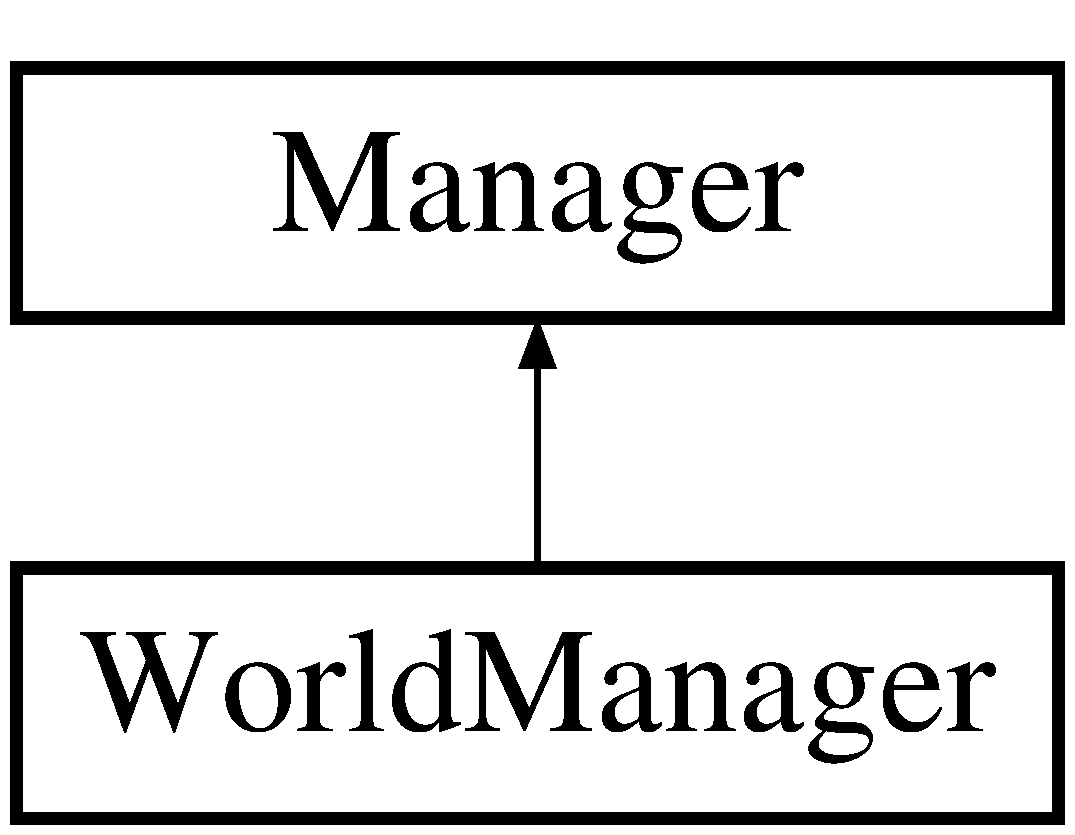
\includegraphics[height=2.000000cm]{class_world_manager}
\end{center}
\end{figure}
\subsection*{Public Member Functions}
\begin{DoxyCompactItemize}
\item 
\hyperlink{class_box}{Box} \hyperlink{class_world_manager_a035099ac90a1f8cf0feb1650e02b3b7a}{get\+Bounds} () const 
\item 
void \hyperlink{class_world_manager_a4e39ad0a294f62d834a7e58f676fe5e6}{set\+Bounds} (\hyperlink{class_box}{Box} bounds)
\item 
\hyperlink{class_box}{Box} \hyperlink{class_world_manager_a54a25642fa5f666c7e6b8e3d668e13b3}{get\+View} () const 
\item 
void \hyperlink{class_world_manager_a2513ce622a4fbb25c3dd3139a9445fec}{set\+View} (\hyperlink{class_box}{Box} view)
\item 
void \hyperlink{class_world_manager_adb4eb19ce21ccad04c60e845f4c508a9}{set\+View\+Position} (const \hyperlink{class_i_vector}{I\+Vector} \&position)
\item 
\hyperlink{class_object}{Object} $\ast$ \hyperlink{class_world_manager_aca77cd8dd87db0e454817668b2d0e8ab}{get\+Following} () const 
\item 
void \hyperlink{class_world_manager_a0d29ce2f7ad696283e80e3fd13b5b077}{set\+Following} (\hyperlink{class_object}{Object} $\ast$follow)
\item 
\hyperlink{class_i_vector}{I\+Vector} \hyperlink{class_world_manager_adb6dd142eb66b01eb5104ab496c9517a}{world\+To\+View} (\hyperlink{class_i_vector}{I\+Vector} \&world\+Pos) const 
\item 
\hyperlink{class_i_vector}{I\+Vector} \hyperlink{class_world_manager_abdffd332d31f310f192a3b017d0940ca}{view\+To\+World} (\hyperlink{class_i_vector}{I\+Vector} \&view\+Pos) const 
\item 
int \hyperlink{class_world_manager_a7ad9c0bf4968b08b82d7d7daa159943a}{start\+Up} ()
\item 
void \hyperlink{class_world_manager_a94c6c0dae961c535b6f2f543e029d6b6}{shut\+Down} ()
\item 
int \hyperlink{class_world_manager_aa578d092a54953c07ff31908239db4ba}{add\+Object} (\hyperlink{class_object}{Object} $\ast$obj)
\item 
int \hyperlink{class_world_manager_a31f902aa5a2ece9e2213d9ca9612e783}{remove\+Object} (\hyperlink{class_object}{Object} $\ast$obj)
\item 
int \hyperlink{class_world_manager_a9dfc6db89285c0ff0191e80f238968c4}{add\+To\+Layer\+Pool} (\hyperlink{class_object}{Object} $\ast$obj)
\item 
int \hyperlink{class_world_manager_a36b651e832cb1d874b1412576843259f}{remove\+From\+Pool} (\hyperlink{class_object}{Object} $\ast$obj)
\item 
int \hyperlink{class_world_manager_a00279b75512da5e81ea5d13828b6f912}{mark\+For\+Delete} (\hyperlink{class_object}{Object} $\ast$object)
\item 
bool \hyperlink{class_world_manager_ad5cbaffc272fbf2ad79a7ea6cfbd3cf6}{move\+Object} (\hyperlink{class_object}{Object} $\ast$obj, \hyperlink{class_i_vector}{I\+Vector} position)
\item 
\hyperlink{class_object_list}{Object\+List} \hyperlink{class_world_manager_a07ba6788c3fece725cbb9d4917fb9682}{get\+All\+Objects} (bool inactive=false) const 
\item 
bool \hyperlink{class_world_manager_ac658218a84a78dc0610890a5b486d70d}{is\+Collision} (\hyperlink{class_object}{Object} $\ast$obj, \hyperlink{class_i_vector}{I\+Vector} position, \hyperlink{class_object_list}{Object\+List} $\ast$out\+List)
\item 
int \hyperlink{class_world_manager_a72462c64fa931378504f18a2966c303d}{on\+Event} (\hyperlink{class_event}{Event} $\ast$e) const 
\item 
void \hyperlink{class_world_manager_a0ef5e1e476a80ef7715227c6f3a9b6ec}{update} ()
\item 
void \hyperlink{class_world_manager_a0e2c21775041c6943d3cbcbf88601fe7}{draw} ()
\end{DoxyCompactItemize}
\subsection*{Static Public Member Functions}
\begin{DoxyCompactItemize}
\item 
static \hyperlink{class_world_manager}{World\+Manager} \& \hyperlink{class_world_manager_a911e3c4d33b006b21f15f41e90d192d8}{get\+Instance} ()
\end{DoxyCompactItemize}


\subsection{Detailed Description}
\hyperlink{class_manager}{Manager} class for the world 

\subsection{Member Function Documentation}
\hypertarget{class_world_manager_aa578d092a54953c07ff31908239db4ba}{\index{World\+Manager@{World\+Manager}!add\+Object@{add\+Object}}
\index{add\+Object@{add\+Object}!World\+Manager@{World\+Manager}}
\subsubsection[{add\+Object}]{\setlength{\rightskip}{0pt plus 5cm}int World\+Manager\+::add\+Object (
\begin{DoxyParamCaption}
\item[{{\bf Object} $\ast$}]{obj}
\end{DoxyParamCaption}
)}}\label{class_world_manager_aa578d092a54953c07ff31908239db4ba}
Adds an object to the world 
\begin{DoxyParams}{Parameters}
{\em obj} & The object to add \\
\hline
\end{DoxyParams}
\begin{DoxyReturn}{Returns}
1 if the object was added, 0 if not 
\end{DoxyReturn}
\hypertarget{class_world_manager_a9dfc6db89285c0ff0191e80f238968c4}{\index{World\+Manager@{World\+Manager}!add\+To\+Layer\+Pool@{add\+To\+Layer\+Pool}}
\index{add\+To\+Layer\+Pool@{add\+To\+Layer\+Pool}!World\+Manager@{World\+Manager}}
\subsubsection[{add\+To\+Layer\+Pool}]{\setlength{\rightskip}{0pt plus 5cm}int World\+Manager\+::add\+To\+Layer\+Pool (
\begin{DoxyParamCaption}
\item[{{\bf Object} $\ast$}]{obj}
\end{DoxyParamCaption}
)}}\label{class_world_manager_a9dfc6db89285c0ff0191e80f238968c4}
Adds the object to the current layer pool that it has been assigned 
\begin{DoxyParams}{Parameters}
{\em obj} & The object to add to a layer pool \\
\hline
\end{DoxyParams}
\begin{DoxyReturn}{Returns}
1 if the object was added, 0 otherwise 
\end{DoxyReturn}
\hypertarget{class_world_manager_a0e2c21775041c6943d3cbcbf88601fe7}{\index{World\+Manager@{World\+Manager}!draw@{draw}}
\index{draw@{draw}!World\+Manager@{World\+Manager}}
\subsubsection[{draw}]{\setlength{\rightskip}{0pt plus 5cm}void World\+Manager\+::draw (
\begin{DoxyParamCaption}
{}
\end{DoxyParamCaption}
)}}\label{class_world_manager_a0e2c21775041c6943d3cbcbf88601fe7}
Called once every frame to draw \hypertarget{class_world_manager_a07ba6788c3fece725cbb9d4917fb9682}{\index{World\+Manager@{World\+Manager}!get\+All\+Objects@{get\+All\+Objects}}
\index{get\+All\+Objects@{get\+All\+Objects}!World\+Manager@{World\+Manager}}
\subsubsection[{get\+All\+Objects}]{\setlength{\rightskip}{0pt plus 5cm}{\bf Object\+List} World\+Manager\+::get\+All\+Objects (
\begin{DoxyParamCaption}
\item[{bool}]{inactive = {\ttfamily false}}
\end{DoxyParamCaption}
) const}}\label{class_world_manager_a07ba6788c3fece725cbb9d4917fb9682}
Gets a list of all objects in the world 
\begin{DoxyParams}{Parameters}
{\em inactive} & If true, then also include objects that are inactive \\
\hline
\end{DoxyParams}
\begin{DoxyReturn}{Returns}
A list of the objects 
\end{DoxyReturn}
\hypertarget{class_world_manager_a035099ac90a1f8cf0feb1650e02b3b7a}{\index{World\+Manager@{World\+Manager}!get\+Bounds@{get\+Bounds}}
\index{get\+Bounds@{get\+Bounds}!World\+Manager@{World\+Manager}}
\subsubsection[{get\+Bounds}]{\setlength{\rightskip}{0pt plus 5cm}{\bf Box} World\+Manager\+::get\+Bounds (
\begin{DoxyParamCaption}
{}
\end{DoxyParamCaption}
) const}}\label{class_world_manager_a035099ac90a1f8cf0feb1650e02b3b7a}
Gets the worlds boundary \begin{DoxyReturn}{Returns}
The world boundary 
\end{DoxyReturn}
\hypertarget{class_world_manager_aca77cd8dd87db0e454817668b2d0e8ab}{\index{World\+Manager@{World\+Manager}!get\+Following@{get\+Following}}
\index{get\+Following@{get\+Following}!World\+Manager@{World\+Manager}}
\subsubsection[{get\+Following}]{\setlength{\rightskip}{0pt plus 5cm}{\bf Object} $\ast$ World\+Manager\+::get\+Following (
\begin{DoxyParamCaption}
{}
\end{DoxyParamCaption}
) const}}\label{class_world_manager_aca77cd8dd87db0e454817668b2d0e8ab}
Gets what object the view should follow \begin{DoxyReturn}{Returns}
A pointer to the object that we are following or N\+U\+L\+L if there is none 
\end{DoxyReturn}
\hypertarget{class_world_manager_a911e3c4d33b006b21f15f41e90d192d8}{\index{World\+Manager@{World\+Manager}!get\+Instance@{get\+Instance}}
\index{get\+Instance@{get\+Instance}!World\+Manager@{World\+Manager}}
\subsubsection[{get\+Instance}]{\setlength{\rightskip}{0pt plus 5cm}{\bf World\+Manager} \& World\+Manager\+::get\+Instance (
\begin{DoxyParamCaption}
{}
\end{DoxyParamCaption}
)\hspace{0.3cm}{\ttfamily [static]}}}\label{class_world_manager_a911e3c4d33b006b21f15f41e90d192d8}
Get the singleton instance of this object \begin{DoxyReturn}{Returns}
A reference to the instance of this object 
\end{DoxyReturn}
\hypertarget{class_world_manager_a54a25642fa5f666c7e6b8e3d668e13b3}{\index{World\+Manager@{World\+Manager}!get\+View@{get\+View}}
\index{get\+View@{get\+View}!World\+Manager@{World\+Manager}}
\subsubsection[{get\+View}]{\setlength{\rightskip}{0pt plus 5cm}{\bf Box} World\+Manager\+::get\+View (
\begin{DoxyParamCaption}
{}
\end{DoxyParamCaption}
) const}}\label{class_world_manager_a54a25642fa5f666c7e6b8e3d668e13b3}
Gets the viewport in the world \begin{DoxyReturn}{Returns}
the world view 
\end{DoxyReturn}
\hypertarget{class_world_manager_ac658218a84a78dc0610890a5b486d70d}{\index{World\+Manager@{World\+Manager}!is\+Collision@{is\+Collision}}
\index{is\+Collision@{is\+Collision}!World\+Manager@{World\+Manager}}
\subsubsection[{is\+Collision}]{\setlength{\rightskip}{0pt plus 5cm}bool World\+Manager\+::is\+Collision (
\begin{DoxyParamCaption}
\item[{{\bf Object} $\ast$}]{obj, }
\item[{{\bf I\+Vector}}]{position, }
\item[{{\bf Object\+List} $\ast$}]{out\+List}
\end{DoxyParamCaption}
)}}\label{class_world_manager_ac658218a84a78dc0610890a5b486d70d}
Gets a list of all objects that an object collides with when placed at a position 
\begin{DoxyParams}{Parameters}
{\em obj} & The object to test collision with \\
\hline
{\em position} & The position to place the object at \\
\hline
{\em out\+List} & A list to fill with the objects that obj collised with, if N\+U\+L\+L the function will ignore it \\
\hline
\end{DoxyParams}
\begin{DoxyReturn}{Returns}
True if there are any collisions otherwise false 
\end{DoxyReturn}
\hypertarget{class_world_manager_a00279b75512da5e81ea5d13828b6f912}{\index{World\+Manager@{World\+Manager}!mark\+For\+Delete@{mark\+For\+Delete}}
\index{mark\+For\+Delete@{mark\+For\+Delete}!World\+Manager@{World\+Manager}}
\subsubsection[{mark\+For\+Delete}]{\setlength{\rightskip}{0pt plus 5cm}int World\+Manager\+::mark\+For\+Delete (
\begin{DoxyParamCaption}
\item[{{\bf Object} $\ast$}]{object}
\end{DoxyParamCaption}
)}}\label{class_world_manager_a00279b75512da5e81ea5d13828b6f912}
Marks an object for deletion when it is safe 
\begin{DoxyParams}{Parameters}
{\em object} & The object to delete \\
\hline
\end{DoxyParams}
\begin{DoxyReturn}{Returns}
1 if ok, 0 if not 
\end{DoxyReturn}
\hypertarget{class_world_manager_ad5cbaffc272fbf2ad79a7ea6cfbd3cf6}{\index{World\+Manager@{World\+Manager}!move\+Object@{move\+Object}}
\index{move\+Object@{move\+Object}!World\+Manager@{World\+Manager}}
\subsubsection[{move\+Object}]{\setlength{\rightskip}{0pt plus 5cm}bool World\+Manager\+::move\+Object (
\begin{DoxyParamCaption}
\item[{{\bf Object} $\ast$}]{obj, }
\item[{{\bf I\+Vector}}]{position}
\end{DoxyParamCaption}
)}}\label{class_world_manager_ad5cbaffc272fbf2ad79a7ea6cfbd3cf6}
Attempts to move an object to a location based on its collision model 
\begin{DoxyParams}{Parameters}
{\em obj} & The object to try and move \\
\hline
{\em position} & The position to move it to \\
\hline
\end{DoxyParams}
\begin{DoxyReturn}{Returns}
True if the object was moved, false otherwise 
\end{DoxyReturn}
\hypertarget{class_world_manager_a72462c64fa931378504f18a2966c303d}{\index{World\+Manager@{World\+Manager}!on\+Event@{on\+Event}}
\index{on\+Event@{on\+Event}!World\+Manager@{World\+Manager}}
\subsubsection[{on\+Event}]{\setlength{\rightskip}{0pt plus 5cm}int World\+Manager\+::on\+Event (
\begin{DoxyParamCaption}
\item[{{\bf Event} $\ast$}]{e}
\end{DoxyParamCaption}
) const\hspace{0.3cm}{\ttfamily [virtual]}}}\label{class_world_manager_a72462c64fa931378504f18a2966c303d}
Passes an event to all objects in the world 
\begin{DoxyParams}{Parameters}
{\em e} & The event to pass \\
\hline
\end{DoxyParams}
\begin{DoxyReturn}{Returns}
1 if any objects ate the event, 0 otherwise 
\end{DoxyReturn}


Reimplemented from \hyperlink{class_manager_abfdbe16dc74a246b70a183351e100989}{Manager}.

\hypertarget{class_world_manager_a36b651e832cb1d874b1412576843259f}{\index{World\+Manager@{World\+Manager}!remove\+From\+Pool@{remove\+From\+Pool}}
\index{remove\+From\+Pool@{remove\+From\+Pool}!World\+Manager@{World\+Manager}}
\subsubsection[{remove\+From\+Pool}]{\setlength{\rightskip}{0pt plus 5cm}int World\+Manager\+::remove\+From\+Pool (
\begin{DoxyParamCaption}
\item[{{\bf Object} $\ast$}]{obj}
\end{DoxyParamCaption}
)}}\label{class_world_manager_a36b651e832cb1d874b1412576843259f}
Removes the object from its current layer pool 
\begin{DoxyParams}{Parameters}
{\em obj} & The object to remove \\
\hline
\end{DoxyParams}
\begin{DoxyReturn}{Returns}
1 if the object was removed, 0 otherwise 
\end{DoxyReturn}
\hypertarget{class_world_manager_a31f902aa5a2ece9e2213d9ca9612e783}{\index{World\+Manager@{World\+Manager}!remove\+Object@{remove\+Object}}
\index{remove\+Object@{remove\+Object}!World\+Manager@{World\+Manager}}
\subsubsection[{remove\+Object}]{\setlength{\rightskip}{0pt plus 5cm}int World\+Manager\+::remove\+Object (
\begin{DoxyParamCaption}
\item[{{\bf Object} $\ast$}]{obj}
\end{DoxyParamCaption}
)}}\label{class_world_manager_a31f902aa5a2ece9e2213d9ca9612e783}
Removes the object from the world 
\begin{DoxyParams}{Parameters}
{\em obj} & The object to remove \\
\hline
\end{DoxyParams}
\begin{DoxyReturn}{Returns}
1 if the object was removed, 0 otherwise 
\end{DoxyReturn}
\hypertarget{class_world_manager_a4e39ad0a294f62d834a7e58f676fe5e6}{\index{World\+Manager@{World\+Manager}!set\+Bounds@{set\+Bounds}}
\index{set\+Bounds@{set\+Bounds}!World\+Manager@{World\+Manager}}
\subsubsection[{set\+Bounds}]{\setlength{\rightskip}{0pt plus 5cm}void World\+Manager\+::set\+Bounds (
\begin{DoxyParamCaption}
\item[{{\bf Box}}]{bounds}
\end{DoxyParamCaption}
)}}\label{class_world_manager_a4e39ad0a294f62d834a7e58f676fe5e6}
Sets the world boundary 
\begin{DoxyParams}{Parameters}
{\em bounds} & The new boundary to use for the world \\
\hline
\end{DoxyParams}
\hypertarget{class_world_manager_a0d29ce2f7ad696283e80e3fd13b5b077}{\index{World\+Manager@{World\+Manager}!set\+Following@{set\+Following}}
\index{set\+Following@{set\+Following}!World\+Manager@{World\+Manager}}
\subsubsection[{set\+Following}]{\setlength{\rightskip}{0pt plus 5cm}void World\+Manager\+::set\+Following (
\begin{DoxyParamCaption}
\item[{{\bf Object} $\ast$}]{follow}
\end{DoxyParamCaption}
)}}\label{class_world_manager_a0d29ce2f7ad696283e80e3fd13b5b077}
Sets the object that the view should follow 
\begin{DoxyParams}{Parameters}
{\em follow} & A pointer to the object that we should follow, or N\+U\+L\+L if no object should be followed \\
\hline
\end{DoxyParams}
\hypertarget{class_world_manager_a2513ce622a4fbb25c3dd3139a9445fec}{\index{World\+Manager@{World\+Manager}!set\+View@{set\+View}}
\index{set\+View@{set\+View}!World\+Manager@{World\+Manager}}
\subsubsection[{set\+View}]{\setlength{\rightskip}{0pt plus 5cm}void World\+Manager\+::set\+View (
\begin{DoxyParamCaption}
\item[{{\bf Box}}]{view}
\end{DoxyParamCaption}
)}}\label{class_world_manager_a2513ce622a4fbb25c3dd3139a9445fec}
Sets the viewport in the world 
\begin{DoxyParams}{Parameters}
{\em view} & The new viewport \\
\hline
\end{DoxyParams}
\hypertarget{class_world_manager_adb4eb19ce21ccad04c60e845f4c508a9}{\index{World\+Manager@{World\+Manager}!set\+View\+Position@{set\+View\+Position}}
\index{set\+View\+Position@{set\+View\+Position}!World\+Manager@{World\+Manager}}
\subsubsection[{set\+View\+Position}]{\setlength{\rightskip}{0pt plus 5cm}void World\+Manager\+::set\+View\+Position (
\begin{DoxyParamCaption}
\item[{const {\bf I\+Vector} \&}]{position}
\end{DoxyParamCaption}
)}}\label{class_world_manager_adb4eb19ce21ccad04c60e845f4c508a9}
Sets the position of the viewport 
\begin{DoxyParams}{Parameters}
{\em position} & The new position for the viewport \\
\hline
\end{DoxyParams}
\hypertarget{class_world_manager_a94c6c0dae961c535b6f2f543e029d6b6}{\index{World\+Manager@{World\+Manager}!shut\+Down@{shut\+Down}}
\index{shut\+Down@{shut\+Down}!World\+Manager@{World\+Manager}}
\subsubsection[{shut\+Down}]{\setlength{\rightskip}{0pt plus 5cm}void World\+Manager\+::shut\+Down (
\begin{DoxyParamCaption}
{}
\end{DoxyParamCaption}
)\hspace{0.3cm}{\ttfamily [virtual]}}}\label{class_world_manager_a94c6c0dae961c535b6f2f543e029d6b6}
Called to shut down the world manager, this will clean up all objects 

Reimplemented from \hyperlink{class_manager_a09f0aaf6012be52b75a12fac25370f61}{Manager}.

\hypertarget{class_world_manager_a7ad9c0bf4968b08b82d7d7daa159943a}{\index{World\+Manager@{World\+Manager}!start\+Up@{start\+Up}}
\index{start\+Up@{start\+Up}!World\+Manager@{World\+Manager}}
\subsubsection[{start\+Up}]{\setlength{\rightskip}{0pt plus 5cm}int World\+Manager\+::start\+Up (
\begin{DoxyParamCaption}
{}
\end{DoxyParamCaption}
)\hspace{0.3cm}{\ttfamily [virtual]}}}\label{class_world_manager_a7ad9c0bf4968b08b82d7d7daa159943a}
Called when the world manager is started \begin{DoxyReturn}{Returns}
0 when no errors occurred, $<$ 0 if errors did occur 
\end{DoxyReturn}


Reimplemented from \hyperlink{class_manager_a2a0f0d6810a5a051afd707d83ff1ff36}{Manager}.

\hypertarget{class_world_manager_a0ef5e1e476a80ef7715227c6f3a9b6ec}{\index{World\+Manager@{World\+Manager}!update@{update}}
\index{update@{update}!World\+Manager@{World\+Manager}}
\subsubsection[{update}]{\setlength{\rightskip}{0pt plus 5cm}void World\+Manager\+::update (
\begin{DoxyParamCaption}
{}
\end{DoxyParamCaption}
)}}\label{class_world_manager_a0ef5e1e476a80ef7715227c6f3a9b6ec}
Called once every frame to update objects \hypertarget{class_world_manager_abdffd332d31f310f192a3b017d0940ca}{\index{World\+Manager@{World\+Manager}!view\+To\+World@{view\+To\+World}}
\index{view\+To\+World@{view\+To\+World}!World\+Manager@{World\+Manager}}
\subsubsection[{view\+To\+World}]{\setlength{\rightskip}{0pt plus 5cm}{\bf I\+Vector} World\+Manager\+::view\+To\+World (
\begin{DoxyParamCaption}
\item[{{\bf I\+Vector} \&}]{view\+Pos}
\end{DoxyParamCaption}
) const}}\label{class_world_manager_abdffd332d31f310f192a3b017d0940ca}
Converts a view coordinate to a world coordinate 
\begin{DoxyParams}{Parameters}
{\em view\+Pos} & The view coordinates \\
\hline
\end{DoxyParams}
\begin{DoxyReturn}{Returns}
The world coordinates 
\end{DoxyReturn}
\hypertarget{class_world_manager_adb6dd142eb66b01eb5104ab496c9517a}{\index{World\+Manager@{World\+Manager}!world\+To\+View@{world\+To\+View}}
\index{world\+To\+View@{world\+To\+View}!World\+Manager@{World\+Manager}}
\subsubsection[{world\+To\+View}]{\setlength{\rightskip}{0pt plus 5cm}{\bf I\+Vector} World\+Manager\+::world\+To\+View (
\begin{DoxyParamCaption}
\item[{{\bf I\+Vector} \&}]{world\+Pos}
\end{DoxyParamCaption}
) const}}\label{class_world_manager_adb6dd142eb66b01eb5104ab496c9517a}
Converts a world coordinate to a view coordinate 
\begin{DoxyParams}{Parameters}
{\em world\+Pos} & The world coordinate \\
\hline
\end{DoxyParams}
\begin{DoxyReturn}{Returns}
The view coordinate 
\end{DoxyReturn}


The documentation for this class was generated from the following files\+:\begin{DoxyCompactItemize}
\item 
F\+:/\+Users/\+Benny/git/\+I\+M\+G\+D3000/\+I\+M\+G\+D3000\+Proj3/include/World\+Manager.\+h\item 
F\+:/\+Users/\+Benny/git/\+I\+M\+G\+D3000/\+I\+M\+G\+D3000\+Proj3/lib/src/\+Game/World\+Manager.\+cpp\end{DoxyCompactItemize}

%--- End generated contents ---

% Index
\newpage
\phantomsection
\addcontentsline{toc}{chapter}{Index}
\printindex

\end{document}
